\documentclass{article}

  % packages
    % basic stuff for rendering math
    \usepackage[letterpaper, top=1in, bottom=1in, left=1in, right=1in]{geometry}
    \usepackage[english]{babel}
    \usepackage{amsmath, amssymb} 
    \usepackage{bbm}              % for mathbbm

    % extra math symbols and utilities
    \usepackage{mathtools}        % for extra stuff like \coloneqq
    \usepackage{mathrsfs}         % for extra stuff like \mathsrc{}
    \usepackage{centernot}        % for the centernot arrow 
    \usepackage{bm}               % for better boldsymbol/mathbf 
    \usepackage{enumitem}         % better control over enumerate, itemize
    \usepackage{xr-hyper}
    \usepackage{hyperref}         % for hypertext linking
    \usepackage{fancyvrb}          % for better verbatim environments
    \usepackage{newverbs}         % for texttt{}
    \usepackage{xcolor}           % for colored text 
    \usepackage{listings}         % to include code
    \usepackage{lstautogobble}    % helper package for code
    \usepackage{parcolumns}       % for side by side columns for two column code
    

    % page layout
    \usepackage{fancyhdr}         % for headers and footers 
    \usepackage{lastpage}         % to include last page number in footer 
    \usepackage{parskip}          % for no indentation and space between paragraphs    
    \usepackage[T1]{fontenc}      % to include \textbackslash
    \usepackage{footnote}
    \usepackage{etoolbox}

    % for custom environments
    \usepackage{tcolorbox}        % for better colored boxes in custom environments
    \tcbuselibrary{breakable}     % to allow tcolorboxes to break across pages

    % figures and tables 
    \usepackage{pgfplots}
    \pgfplotsset{compat=1.18}
    \usepackage{float}            % for [H] figure placement
    \usepackage{tikz, tikz-cd}
    \usetikzlibrary{arrows, positioning, calc}
    \usepackage{graphicx}
    \usepackage{caption, subcaption} 
    \usepackage{dcolumn}

    \usepackage[nottoc]{tocbibind}
    \hfuzz=5.002pt                % ignore overfull hbox badness warnings below this limit

  % New and replaced operators
    \DeclareMathOperator{\Tr}{Tr}
    \DeclareMathOperator{\Sym}{Sym}
    \DeclareMathOperator{\Span}{span}
    \DeclareMathOperator{\im}{Im}
    \DeclareMathOperator{\Div}{div}
    \DeclareMathOperator{\curl}{curl}
    \DeclareMathOperator{\GL}{GL}
    \DeclareMathOperator{\SL}{SL}
    \DeclareMathOperator{\GA}{GA}
    \DeclareMathOperator{\std}{std}
    \DeclareMathOperator{\Cov}{Cov}
    \DeclareMathOperator{\Var}{Var}
    \DeclareMathOperator{\Corr}{Corr}
    \DeclareMathOperator{\Int}{Int}
    \DeclareMathOperator{\Id}{Id}
    \DeclareMathOperator{\Lie}{Lie}
    \DeclareMathOperator{\Hom}{Hom}
    \DeclareMathOperator{\Alt}{Alt}
    \DeclareMathOperator{\rank}{rank}
    \DeclareMathOperator{\conv}{conv}
    \DeclareMathOperator{\aff}{aff}
    \DeclareMathOperator{\arccot}{arccot}

  % Custom Environments
    \tcbset{
      colframe = black,
      colback  = white,
      coltitle = black,
      colbacktitle = black!10,
      breakable, 
      arc=0mm,
      boxrule=1pt,
      left=8pt,
      right=8pt,
      top=6pt,
      bottom=6pt,
      before skip=12pt,
      after skip=12pt,
      bottomrule at break=-1pt,
      toprule at break=-1pt,
      fonttitle=\bfseries,
    }
    % adds an entry for a theorem/definition/etc. to the table of contents (level of subsubsection)
    % usage: \tocentry{Kind}{number}{optional name}
    \setcounter{tocdepth}{3}
    \hypersetup{bookmarksdepth=2}  % no PDF bookmarks for theorem-level entries (avoids hyperref warnings)
    \newcommand{\tocentry}[3]{%
      \phantomsection
      \ifstrempty{#3}{%
        \addcontentsline{toc}{subsubsection}{#1 #2}%
      }{%
        \addcontentsline{toc}{subsubsection}{#1 #2 (#3)}%
      }%
    }

    % smaller text for non-section entries in the table of contents
    \makeatletter
    \let\origl@subsection\l@subsection
    \let\origl@subsubsection\l@subsubsection
    \renewcommand*\l@subsection[2]{{\small\origl@subsection{#1}{#2}}}
    \renewcommand*\l@subsubsection[2]{{\footnotesize\origl@subsubsection{#1}{#2}}}
    \makeatother

    \newcounter{question}[section]
    \renewcommand{\thequestion}{\thesection.\arabic{question}}
    \NewDocumentEnvironment{question}{O{} o}{%
      \refstepcounter{question}%
      \ifstrempty{#1}{%
        \begin{tcolorbox}[title=\textbf{Question \thequestion}]%
      }{%
        \IfValueTF{#2}{%
          \begin{tcolorbox}[title=\textbf{Question \thequestion~(#1)}, label={#2}]%
        }{%
          \begin{tcolorbox}[title=\textbf{Question \thequestion~(#1)}]%
        }%
      }%
    }{%
      \end{tcolorbox}%
    }

    \newcounter{exercise}[section]
    \renewcommand{\theexercise}{\thesection.\arabic{exercise}}
    \NewDocumentEnvironment{exercise}{O{} o}{%
      \refstepcounter{exercise}%
      \ifstrempty{#1}{%
        \begin{tcolorbox}[title=\textbf{Exercise \theexercise}]%
      }{%
        \IfValueTF{#2}{%
          \begin{tcolorbox}[title=\textbf{Exercise \theexercise~(#1)}, label={#2}]%
        }{%
          \begin{tcolorbox}[title=\textbf{Exercise \theexercise~(#1)}]%
        }%
      }%
    }{%
      \end{tcolorbox}%
    }

    \newtcolorbox[auto counter, number within=section]{solution}[1][]
    {
      before skip = -7pt,
      before upper = \textit{Solution. },
    }

    \newcounter{theorem}[section]
    \renewcommand{\thetheorem}{\thesection.\arabic{theorem}}

    \NewDocumentEnvironment{lemma}{O{} o}{%
      \refstepcounter{theorem}%
      \tocentry{Lemma}{\thetheorem}{#1}%
      \ifstrempty{#1}{%
        \begin{tcolorbox}[title=\textbf{Lemma \thetheorem}]%
      }{%
        \IfValueTF{#2}{%
          \begin{tcolorbox}[title=\textbf{Lemma \thetheorem~(#1)}, label={#2}]%
        }{%
          \begin{tcolorbox}[title=\textbf{Lemma \thetheorem~(#1)}]%
        }%
      }%
    }{%
      \end{tcolorbox}%
    }

    \NewDocumentEnvironment{theorem}{O{} o}{%
      \refstepcounter{theorem}%
      \tocentry{Theorem}{\thetheorem}{#1}%
      \ifstrempty{#1}{%
        \begin{tcolorbox}[title=\textbf{Theorem \thetheorem}]%
      }{%
        \IfValueTF{#2}{%
          \begin{tcolorbox}[title=\textbf{Theorem \thetheorem~(#1)}, label={#2}]%
        }{%
          \begin{tcolorbox}[title=\textbf{Theorem \thetheorem~(#1)}]%
        }%
      }%
    }{%
      \end{tcolorbox}%
    }

    \NewDocumentEnvironment{corollary}{O{} o}{%
      \refstepcounter{theorem}%
      \tocentry{Corollary}{\thetheorem}{#1}%
      \ifstrempty{#1}{%
        \begin{tcolorbox}[title=\textbf{Corollary \thetheorem}]%
      }{%
        \IfValueTF{#2}{%
          \begin{tcolorbox}[title=\textbf{Corollary \thetheorem~(#1)}, label={#2}]%
        }{%
          \begin{tcolorbox}[title=\textbf{Corollary \thetheorem~(#1)}]%
        }%
      }%
    }{%
      \end{tcolorbox}%
    }

    \newtcolorbox[auto counter, number within=section]{proof}[1][]
    {
      before skip = -7pt,
      before upper = \textit{Proof. },
    }

    \newcounter{definition}[section]
    \renewcommand{\thedefinition}{\thesection.\arabic{definition}}
    \NewDocumentEnvironment{definition}{O{} o}{%
      \refstepcounter{definition}%
      \tocentry{Definition}{\thedefinition}{#1}%
      \ifstrempty{#1}{%
        \begin{tcolorbox}[title=\textbf{Definition \thedefinition}]%
      }{%
        \IfValueTF{#2}{%
          \begin{tcolorbox}[title=\textbf{Definition \thedefinition~(#1)}, label={#2}]%
        }{%
          \begin{tcolorbox}[title=\textbf{Definition \thedefinition~(#1)}]%
        }%
      }%
    }{%
      \end{tcolorbox}%
    }

    \newcounter{example}[section]
    \renewcommand{\theexample}{\thesection.\arabic{example}}
    \NewDocumentEnvironment{example}{O{} o}{%
      \refstepcounter{example}%
      \tocentry{Example}{\theexample}{#1}%
      \ifstrempty{#1}{%
        \begin{tcolorbox}[title=\textbf{Example \theexample}]%
      }{%
        \IfValueTF{#2}{%
          \begin{tcolorbox}[title=\textbf{Example \theexample~(#1)}, label={#2}]%
        }{%
          \begin{tcolorbox}[title=\textbf{Example \theexample~(#1)}]%
        }%
      }%
    }{%
      \end{tcolorbox}%
    }

    \newcounter{code}[section]
    \renewcommand{\thecode}{\thesection.\arabic{code}}
    \NewDocumentEnvironment{code}{O{} o}{%
      \refstepcounter{code}%
      \ifstrempty{#1}{%
        \begin{tcolorbox}[title=\textbf{Code \thecode}]%
      }{%
        \IfValueTF{#2}{%
          \begin{tcolorbox}[title=\textbf{Code \thecode~(#1)}, label={#2}]%
        }{%
          \begin{tcolorbox}[title=\textbf{Code \thecode~(#1)}]%
        }%
      }%
    }{%
      \end{tcolorbox}%
    } 

    \definecolor{dkgreen}{rgb}{0,0.6,0}
    \definecolor{gray}{rgb}{0.5,0.5,0.5}
    \definecolor{mauve}{rgb}{0.58,0,0.82}
    \definecolor{lightgray}{gray}{0.93}

    % default options for listings (for code)
    \lstset{
      autogobble,
      frame=ltbr,
      language=C,                           % the language of the code
      aboveskip=3mm,
      belowskip=3mm,
      showstringspaces=false,
      columns=fullflexible,
      keepspaces=true,
      basicstyle={\small\ttfamily},
      numbers=left,
      firstnumber=1,                        % start line number at 1
      numberstyle=\tiny\color{gray},
      keywordstyle=\color{blue},
      commentstyle=\color{dkgreen},
      stringstyle=\color{mauve},
      backgroundcolor=\color{lightgray}, 
      breaklines=true,                      % break lines
      breakatwhitespace=true,
      tabsize=3, 
      xleftmargin=2em, 
      framexleftmargin=1.5em, 
      stepnumber=1
    }

  % Page style
    \pagestyle{fancy}
    \fancyhead[L]{Smooth Manifolds}
    \fancyhead[C]{Muchang Bahng}
    \fancyhead[R]{Fall 2021} 
    \fancyfoot[C]{\thepage / \pageref{LastPage}}
    \renewcommand{\footrulewidth}{0.4pt}          % the footer line should be 0.4pt wide
    \renewcommand{\thispagestyle}[1]{}  % needed to include headers in title page

  % external documents
    \externaldocument[log-]{../Logic/paper}[https://mbahng.com/Math/Logic/paper.pdf]
    \externaldocument[st-]{../Set_Theory/paper}[https://mbahng.com/Math/Set_Theory/paper.pdf]
    \externaldocument[cat-]{../Category_Theory/paper}[https://mbahng.com/Math/Category_Theory/paper.pdf]
    \externaldocument[alg-]{../Abstract_Algebra/paper}[https://mbahng.com/Math/Abstract_Algebra/paper.pdf]
    \externaldocument[pst-]{../Point_Set_Topology/paper}[https://mbahng.com/Math/Point_Set_Topology/paper.pdf]
    \externaldocument[at-]{../Algebraic_Topology/paper}[https://mbahng.com/Math/Algebraic_Topology/paper.pdf]
    \externaldocument[lin-]{../Linear_Algebra/paper}[https://mbahng.com/Math/Linear_Algebra/paper.pdf]
    \externaldocument[real-]{../Univariate_Analysis/paper}[https://mbahng.com/Math/Univariate_Analysis/paper.pdf]
    \externaldocument[mv-]{../Multivariate_Analysis/paper}[https://mbahng.com/Math/Multivariate_Analysis/paper.pdf]
    \externaldocument[cx-]{../Complex_Analysis/paper}[https://mbahng.com/Math/Complex_Analysis/paper.pdf]
    \externaldocument[mt-]{../Measure_Theory/paper}[https://mbahng.com/Math/Measure_Theory/paper.pdf]
    \externaldocument[ode-]{../Ordinary_Differential_Equations/paper}[https://mbahng.com/Math/Ordinary_Differential_Equations/paper.pdf]
    \externaldocument[pde-]{../Partial_Differential_Equations/paper}[https://mbahng.com/Math/Partial_Differential_Equations/paper.pdf]
    \externaldocument[fa-]{../Functional_Analysis/paper}[https://mbahng.com/Math/Functional_Analysis/paper.pdf]
    \externaldocument[prob-]{../Probability_Theory/paper}[https://mbahng.com/Math/Probability_Theory/paper.pdf]
    \externaldocument[sp-]{../Stochastic_Processes/paper}[https://mbahng.com/Math/Stochastic_Processes/paper.pdf]
    \externaldocument[com-]{../Concentration_of_Measure/paper}[https://mbahng.com/Math/Concentration_of_Measure/paper.pdf]

\begin{document}

\title{Smooth Manifolds}
\author{Muchang Bahng}
\date{Fall 2021}

\maketitle
\tableofcontents
\pagebreak

Manifolds are invaluable in generalizing multiple ideas. For example, it allows us to generalize the concepts to calculus to spaces that are not only globally, but \textit{locally} Euclidean. 

\section{Smooth Manifolds}

  \subsection{Topological Manifolds and Topological Properties}

    \begin{definition}[Topological Manifold, Coordinate Chart, Atlas]
      \label{def:topological-manifold-coordinate-chart-atlas}
      Suppose $M$ is a topological space. $M$ is a (real) \textit{topological manifold of dimension $N$} if
      \begin{enumerate}
        \item $M$ is Hausdorff: for every pair of points $p, q \in M$, there exists disjoint open subsets $U, V \subset M$ such that $p \in U$, $q \in V$. 

        \item $M$ is second countable: There exists a countable basis for the topology of $M$. 

        \item $M$ is \hyperref[pst-def:locally-homeomorphic]{locally homeomorphic} to $\mathbb{R}^N$: There exists a covering of \hyperref[pst-def:open-set]{open sets} in $M$ where each open set is homeomorphic to an open set in $\mathbb{R}^N$. The visual below shows a 1-dimensional and 2-dimensional manifold. 

        \begin{center}
          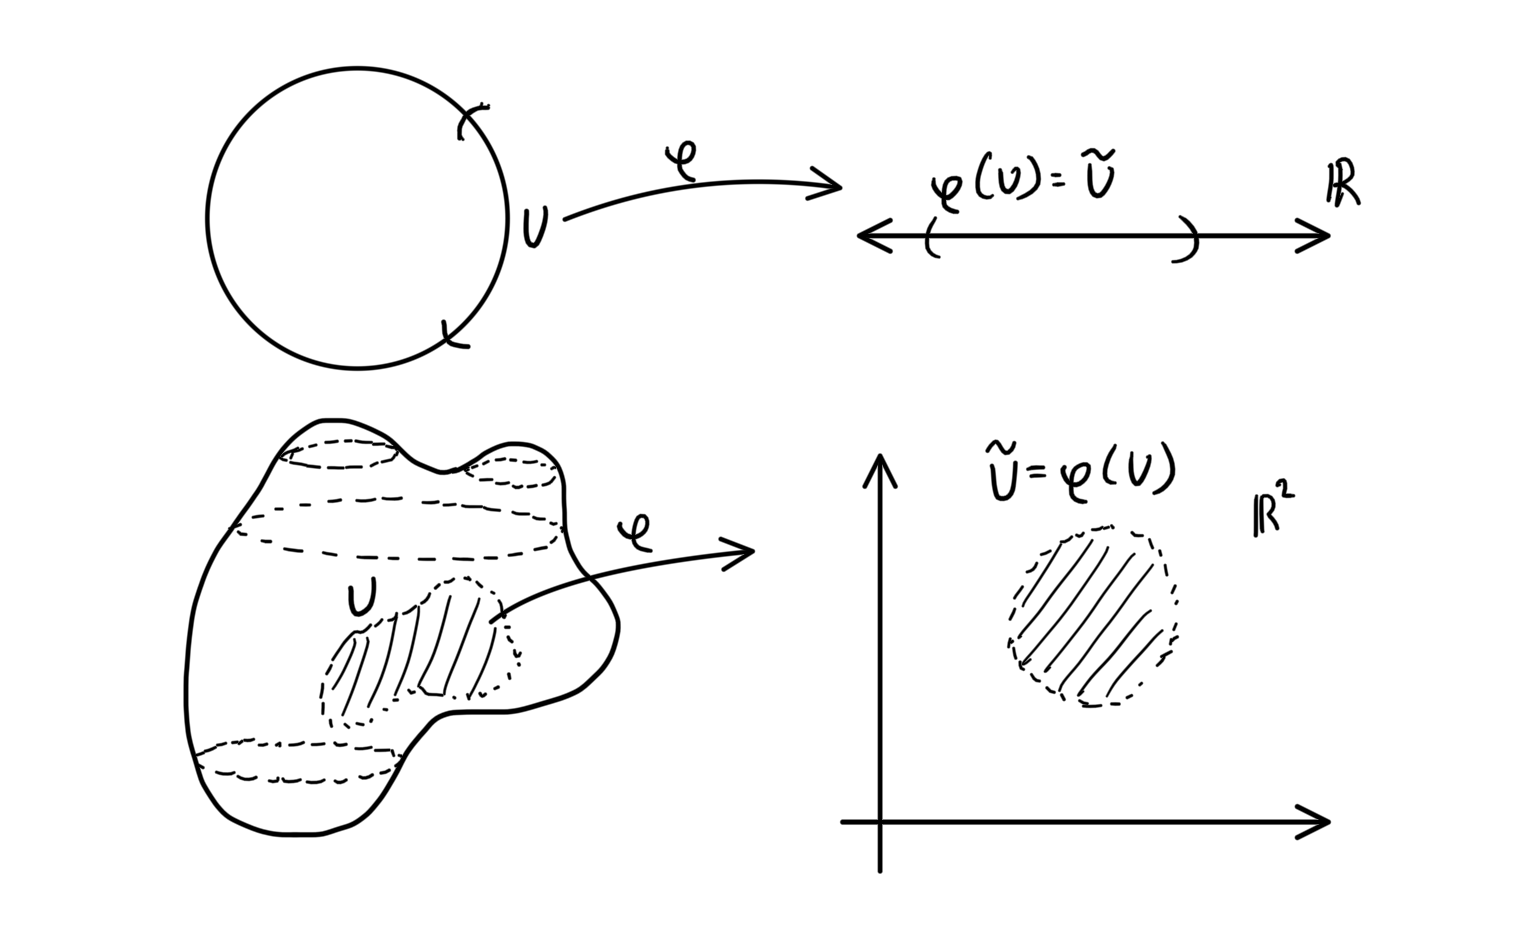
\includegraphics[scale=0.20]{img/1_2_dim_Manifold_Coordinate_Chart.PNG}
        \end{center}
      \end{enumerate}

      Given open cover $U_1, \ldots, U_n$ with their respective \hyperref[pst-def:homeomorphism]{homeomorphism} maps $\varphi_1, \ldots, \varphi_n$ where

        \begin{equation}
          \varphi_i : U_i \longrightarrow \mathbb{R}^n
        \end{equation}

      and component maps

        \begin{equation}
          \varphi_i \equiv (x_{i1}, x_{i2}, ..., x_{in})
        \end{equation}

      their pairs $(U_i, \varphi_i)$ are called \textit{coordinate charts}. The collection of all coordinate charts 

        \begin{equation}
          \mathcal{A} = \{(U_i, \varphi_i)\}_{i=1}^n
        \end{equation}

      is called the \textit{atlas} of $M$. 
    \end{definition}

    Note that the Hausdorff and second-countability condition is sometimes ommitted from the definition of a manifold, but we keep it since: 

    \begin{enumerate}
      \item many manifolds in nature have these properties. 
      \item we can deduce must more interesting properties about manifolds with these assumptions.
    \end{enumerate}

    \begin{theorem}[Product Manifolds]
      \label{thm:product-manifolds}
      Let $M_1, M_2, ..., M_n$ be topological manifolds of dimensions $m_1, m_2$ $...m_n$, respectively. Then, the product space 

        \begin{equation}
          \prod_{i=1}^n M_i
        \end{equation}

      is also a topological manifold with 

      \begin{equation}
        \dim{\prod_{i=1}^n M_i} = \sum_{i=1}^n m_i
      \end{equation}

      \begin{center}
        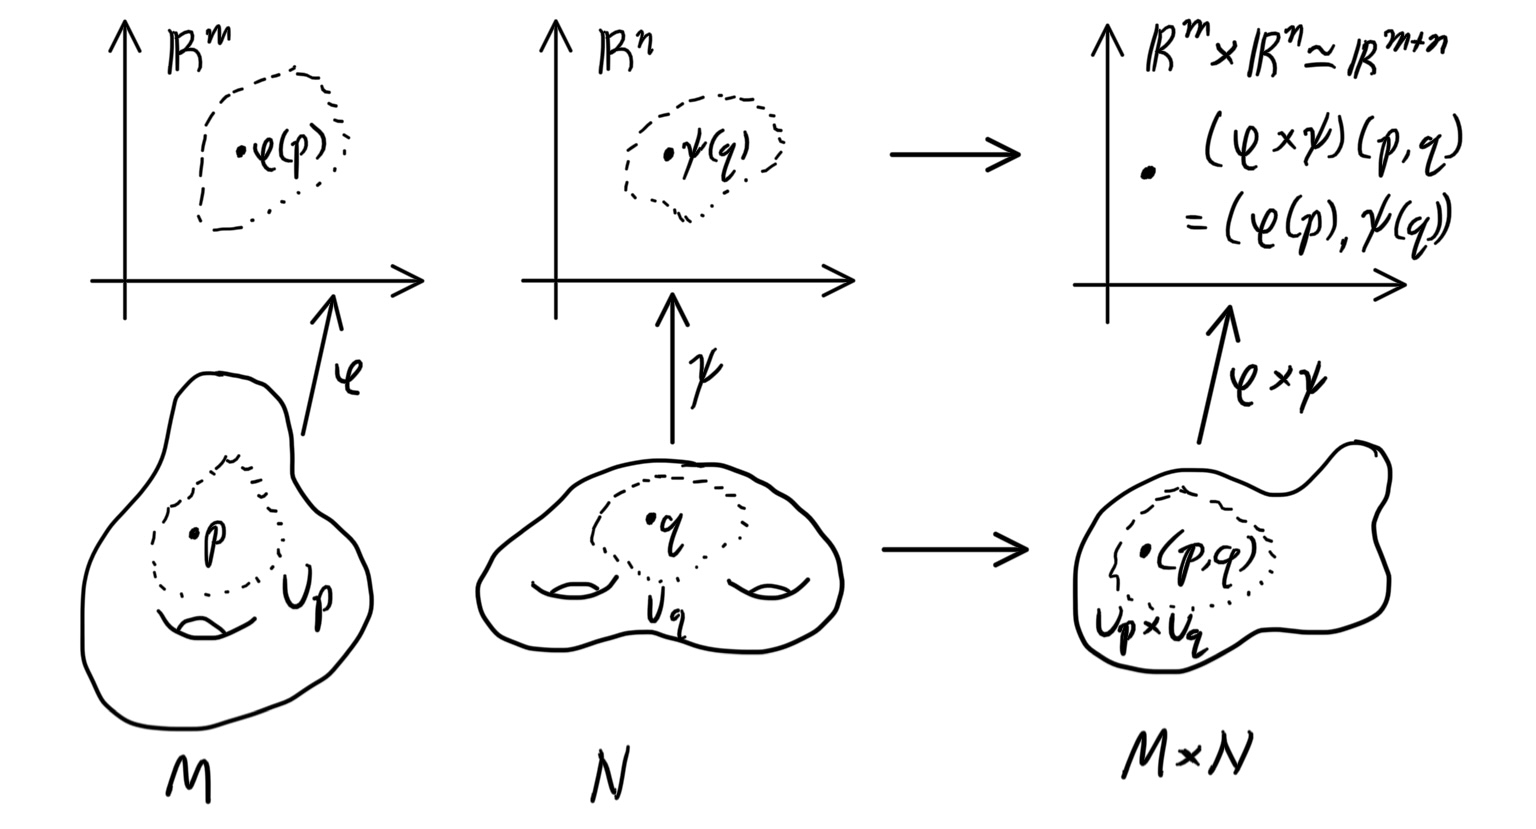
\includegraphics[scale=0.25]{img/Product_Manifolds.PNG}
      \end{center}
    \end{theorem}

    \begin{example}[Graphs of Continuous Functions]
      \label{ex:graphs-of-continuous-functions}
      Given a continuous function $f: U \longrightarrow \mathbb{R}^m$, its graph

        \begin{equation}
          \Gamma (f) \equiv \{(x, y) \in \mathbb{R}^n \times \mathbb{R}^m \; | \;  x\in U, y = f(x)\}
        \end{equation}

      with the \hyperref[pst-def:subspace-topology]{subspace topology} is a topological manifold. Actually, this manifold is \textit{globally homeomorphic} to an \hyperref[pst-def:open-set]{open set} in $\mathbb{R}^n$, meaning that this is trivially a manifold. 
    \end{example}

    \begin{example}[Unit Sphere]
      \label{ex:unit-sphere}
      The unit sphere $S^n$ is a topological manifold since we can construct an atlas of charts formed by the \hyperref[at-thm:stereographic-projection]{stereographic projection}. We show the stereographic projection for a $1$-sphere. 

      \begin{center}
        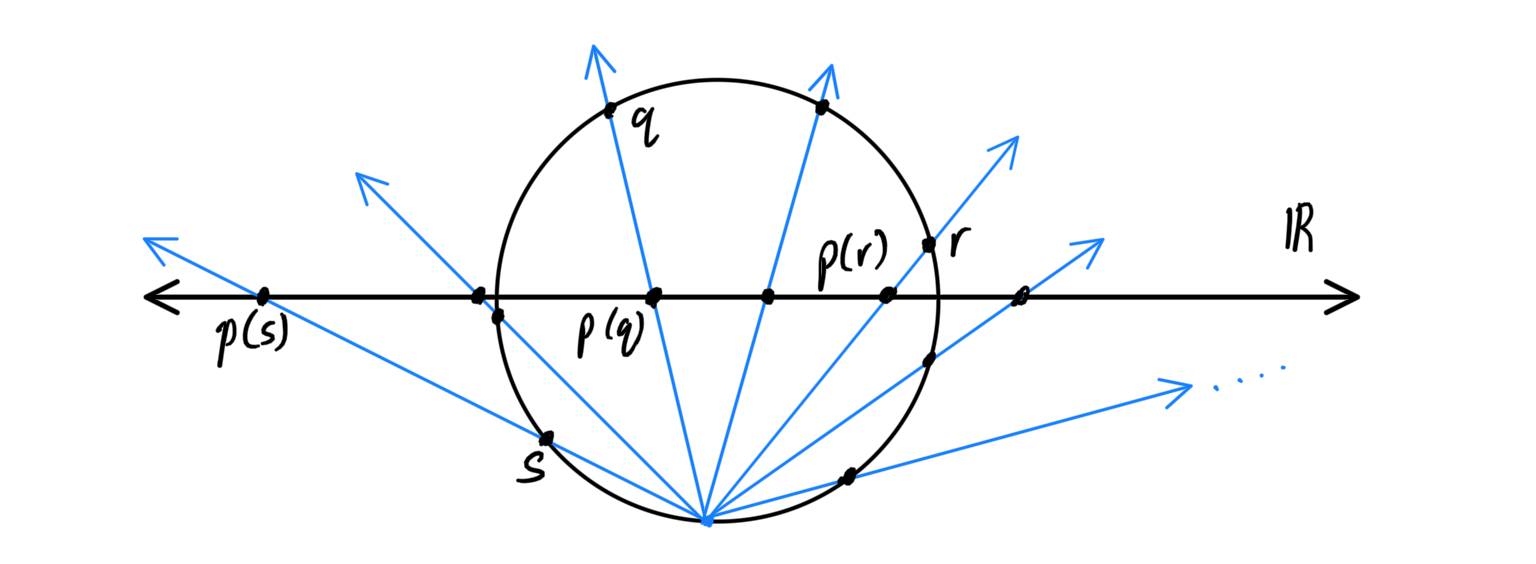
\includegraphics[scale=0.25]{img/1_dim_Stereographic_Projection.PNG}
      \end{center}
    \end{example}

    \begin{example}[$S^n$ Is Not Homeomorphic to $\mathbb{R}^n$]
      \label{ex:sn-is-not-homeomorphic-to-rn}
      The $n$-sphere with the induced open ball topology of $\mathbb{R}^{n+1}$ is not homeomorphic to $\mathbb{R}^{n}$ since $S^{n}$ is compact and $\mathbb{R}^{n}$ is not. However, the $n$-sphere with one point $p \in S^{n}$ removed, $(S^{n} \setminus{\{p\}}, \tau_{\mathbb{R}^{n+1}} |_{S^{n} \setminus{\{p\}}})$ \textit{is} homeomorphic to $\mathbb{R}^{n}$ and is also not compact. We can visualize this \hyperref[pst-def:homeomorphism]{homeomorphism} by imagining the "hole" getting larger and stretching $S^{2}$ out to "look like" $\mathbb{R}^{2}$.
    \end{example}

    \begin{example}[The $n$-Torus as a Product Manifold]
      \label{ex:the-n-torus-as-a-product-manifold}
      The $n$-torus, defined

        \begin{equation}
          \mathbb{T}^n \equiv \prod_n S^1
        \end{equation}

      is a product manifold. 
    \end{example}

    We end this section by stating a theorem that gives topological manifolds a nice basis structure. Recall that a subset $U$ in a topological space $X$ is said to be \textit{precompact} if the closure $\bar{U}$ is compact. 

    \begin{lemma}[Basis of Topological Manifolds]
      \label{thm:basis-of-topological-manifolds}
      Every topological manifold has a countable basis of precompact coordinate balls. 
      \begin{center}
        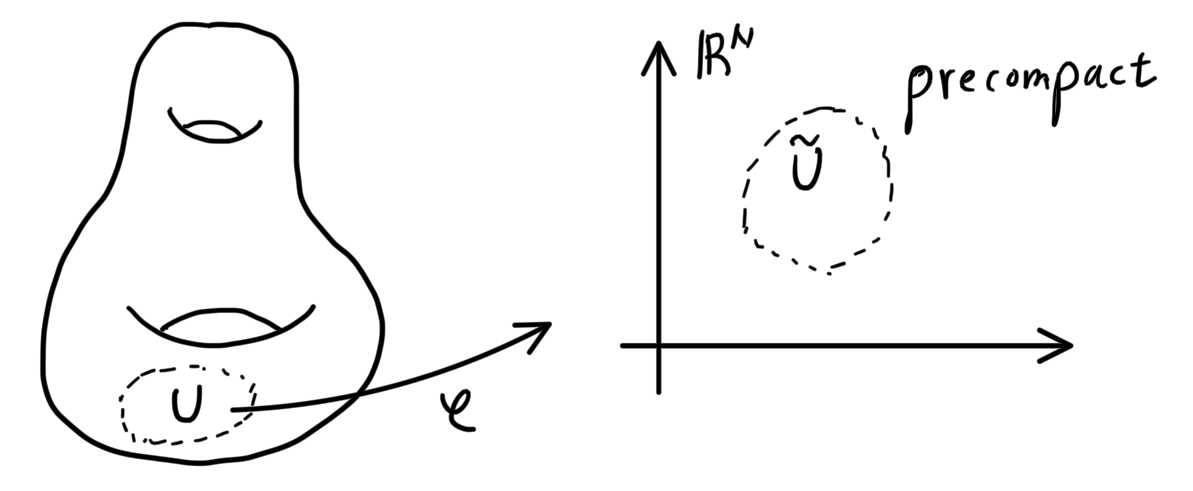
\includegraphics[scale=0.23]{img/Precompact_Basis.PNG}
      \end{center}
    \end{lemma}

    \begin{lemma}[Fundamental Groups of Topological Manifolds]
      \label{thm:fundamental-groups-of-topological-manifolds}
      The \hyperref[at-def:fundamental-group]{fundamental group} of any topological manifold is countable. 
    \end{lemma}

  \subsection{Smooth Structures}

    Note that even though topological manifolds bear some resemblance to Euclidean space, we cannot do calculus on them since derivatives are not invariant under \hyperref[pst-def:homeomorphism]{homeomorphisms}. For example, compare the two homeomorphisms $\varphi_1, \varphi_2: \mathbb{R}^2 \longrightarrow \mathbb{R}^2$ (shown by visualizing the images of the grid lines), where

    \begin{equation}
      \varphi_1 (u, v) = (u, v) \;\;\;\;\;\;\;\;\;\;\;\;\;\;\;\;\;\;\;\; \varphi_2 (u, v) = (u^{1/3}, v^{1/3})
    \end{equation}

    \begin{center}
      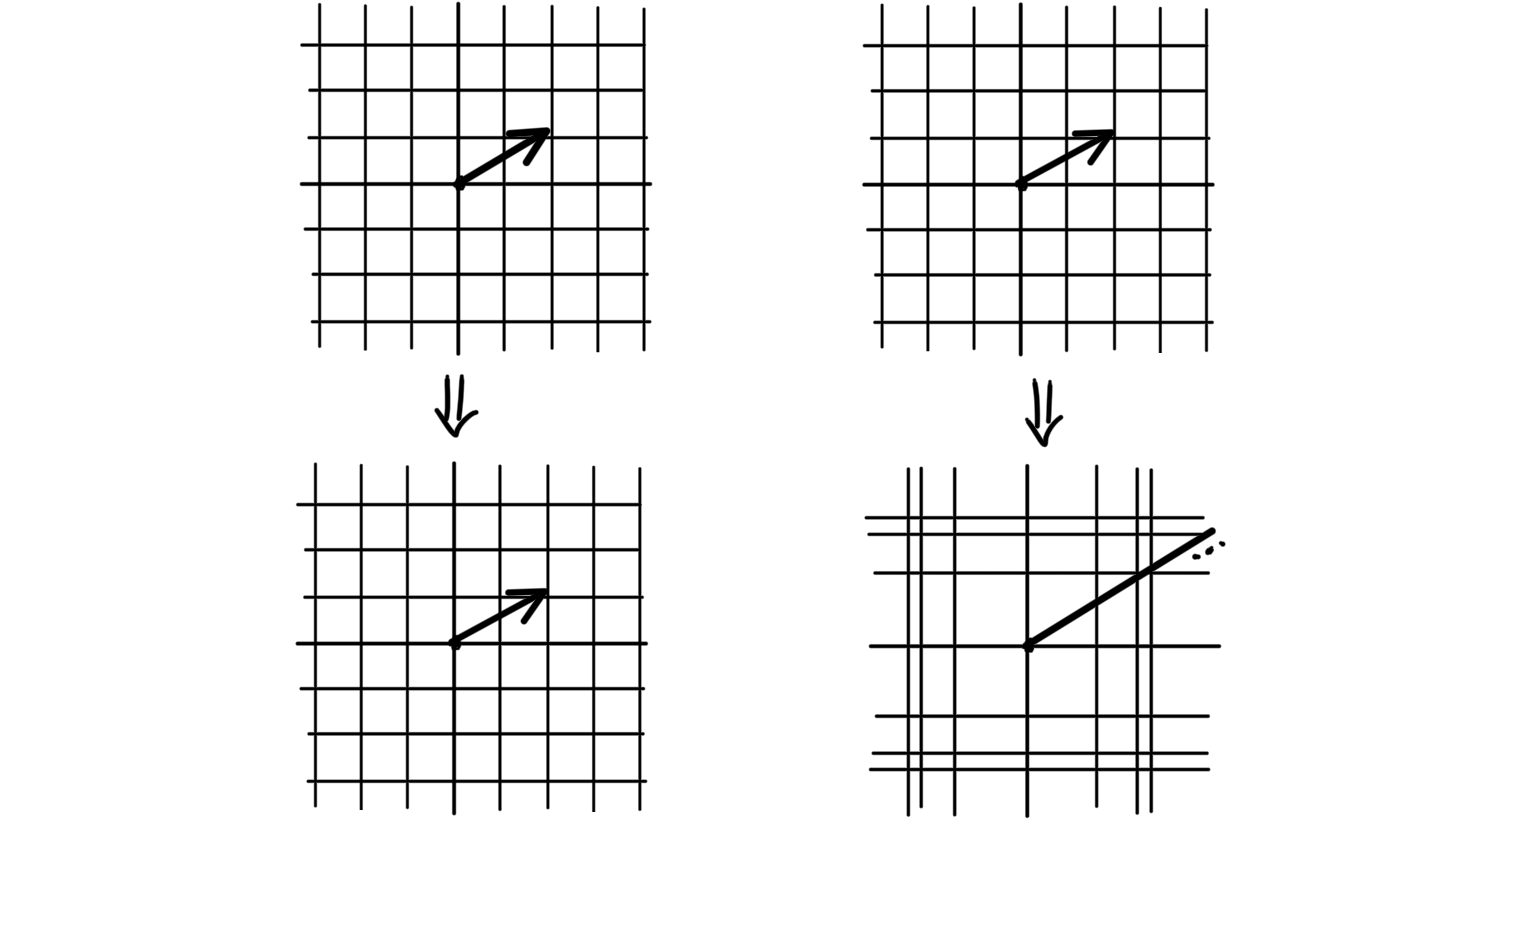
\includegraphics[scale=0.22]{img/Nonexistent_Derivative_Homeomorphism.PNG}
    \end{center}

    Given function $f: M \longrightarrow \mathbb{R}^m$, if topological manifold $M$ has chart $\varphi_1$, $f$ will be considered smooth at $\varphi^{-1}(0)$, but if $M$ has chart $\varphi_2$, $f$ will not be considered smooth at $\varphi^{-2}(0)$. 

    Clearly, it is a problem if two different charts around a point gives contradicting things about its smoothness. We can fix this by introducing a structure that makes smoothness invariant. First, recall the definition of a diffeomorphism. 

    \begin{definition}[Diffeomorphism]
      \label{def:diffeomorphism}
      If smooth $f: U \subset \mathbb{R}^n \longrightarrow V \subset \mathbb{R}^m$ is bijective and has a smooth inverse map, then $f$ is said to be a \textit{diffeomorphism}. That is, a diffeomorphism is a \hyperref[pst-def:homeomorphism]{homeomorphism} where both the function and its inverse is smooth. More specifically, 
      \begin{enumerate}
        \item If $f, f^{-1}$ is of class $C^k$, then it is a $C^k$-diffeomorphism. 
        \item $f, f^{-1}$ is of class $C^\infty$, then it is a $C^\infty$-diffeomorphism, or a smooth diffeomorphism.
      \end{enumerate}
    \end{definition}

    \begin{definition}[Transition Maps, Smooth Atlases]
      \label{def:transition-maps-smooth-atlases}
      Let $M$ be a topological manifold with $(U, \varphi), (V, \psi)$ two charts such that $U \cap V \neq \emptyset$. Then, the composite map (between Euclidean spaces)
      \begin{equation}
        \psi \circ \varphi^{-1} : \varphi(U \cap V) \longrightarrow \psi(U \cap V)
      \end{equation}
      is called the \textit{transition map} from $\varphi$ to $\psi$. 
      \begin{center}
          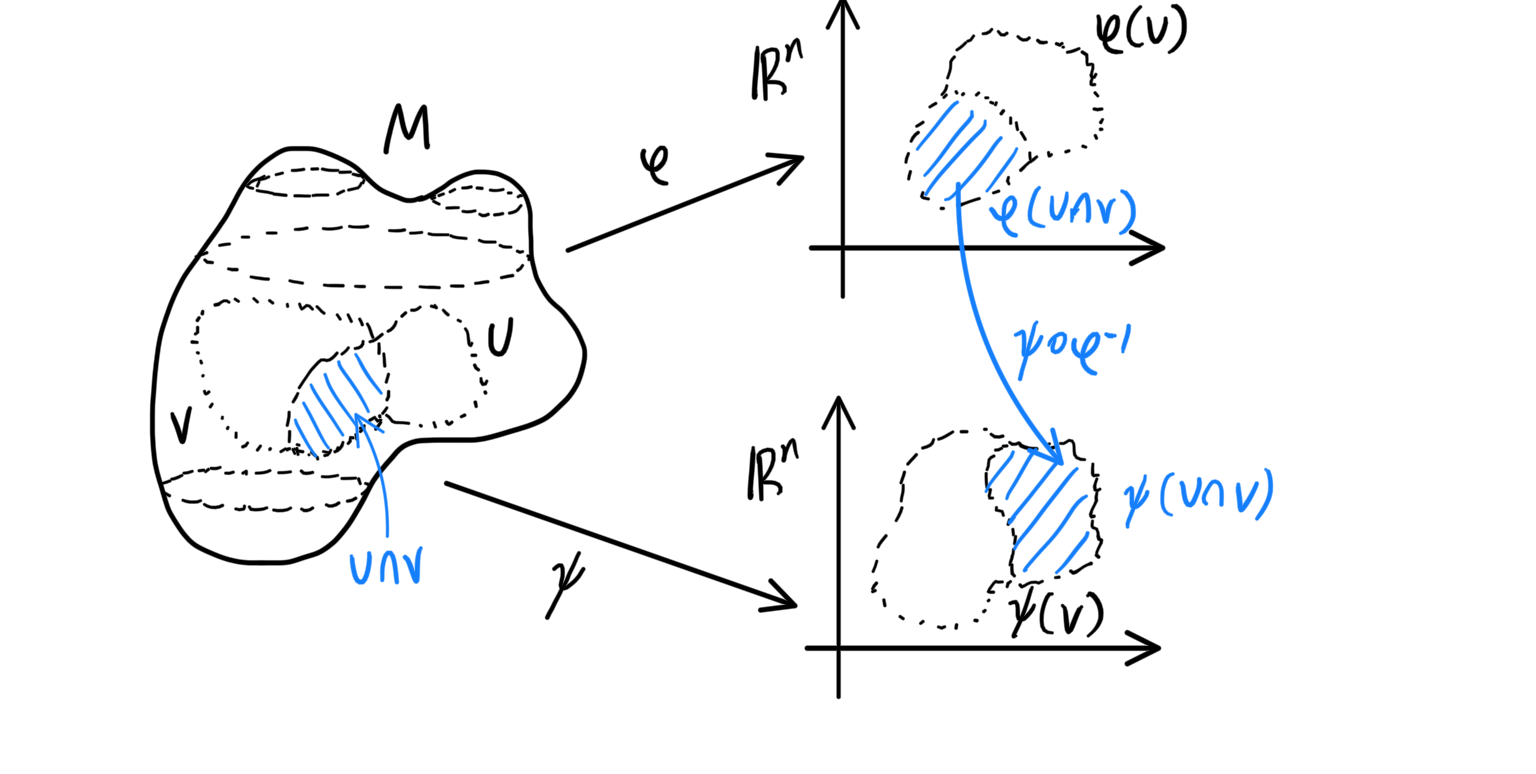
\includegraphics[scale=0.27]{img/Transition_Map.PNG}
      \end{center}
      The two charts are said to be smoothly (or $C^k$) compatible if either 
      \begin{enumerate}
          \item $U \cap V = \emptyset$, or
          \item the transition map $\psi \circ \varphi^{-1}$ is a smooth (or $C^k$) \hyperref[def:diffeomorphism]{diffeomorphism}. Since $\psi \circ \varphi^{-1}$ is a map between Euclidean spaces, this means that $\psi \circ \varphi^{-1}$ has continuous \hyperref[mv-def:partial-derivative]{partial derivatives}. 
      \end{enumerate}
      An atlas $\mathcal{A}$ is called a \textit{smooth ($C^k$) atlas} if any 2 charts in $\mathcal{A}$ are smoothly ($C^k$) compatible with each other. 
    \end{definition}

    \begin{example}[Transition Map between Stereographic Projections]
      \label{ex:transition-map-between-stereographic-projections}
      A transition map can be defined between two stereographic projections of the 1-sphere $\delta_{1}: S^{1} \setminus{\{p\}} \longrightarrow \mathbb{R}$ and $\delta_{2}: S^{1} \setminus{\{q\}} \longrightarrow \mathbb{R}$, where $p$ and $q$ are diametrically opposite points of $S^{1}$. By placing $\mathbb{R}$ within $S^{1}$ orthogonal to the line segment $\overline{PQ}$ and intersecting the center of $S^{1}$, we find that the transition function $\delta_{1} \circ \delta_{2}^{-1}(n) = \delta_{2} \circ \delta_{1}^{-1}(n) = \frac{1}{n}$.  
      \begin{center}
        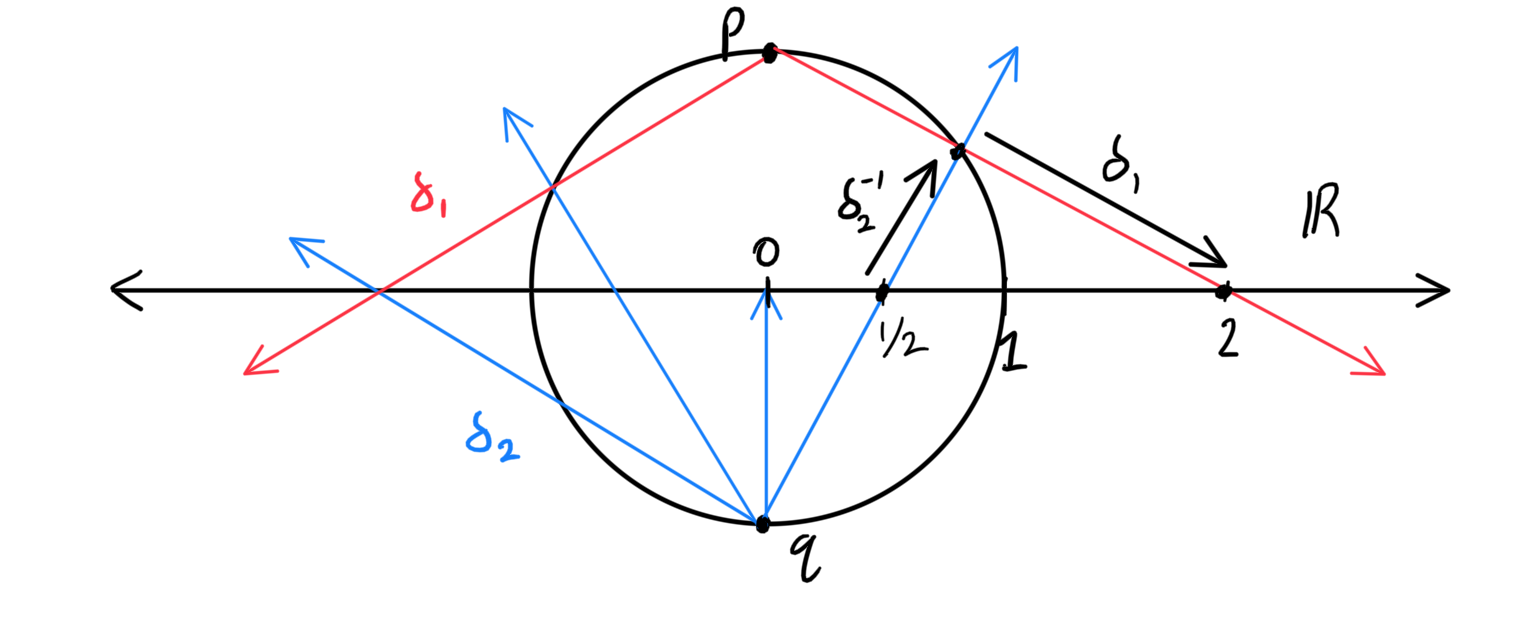
\includegraphics[scale=0.25]{img/1_dim_projection_transition_function.PNG}
      \end{center}
    \end{example}

    Let's go back to our example problem earlier. Given an open neighborhood $M$ around $0 \in \mathbb{R}^2$, the two (global) charts $\varphi_1, \varphi_2$ are not smoothly compatible since 
      \begin{equation}
        (\varphi_2 \circ \varphi_1^{-1})(u, v) = (u^{1/3}, v^{1/3})
      \end{equation}
    is not smooth. Therefore, they cannot be a part of the same smooth atlas. 

    Our previous problem hints at another one: Which atlas is the "right" one? In general, there will be many possible choices of atlases that give the "same" smooth structure. The 3 following atlases shown below (consisting of one global chart, for simplicity), are all viable. 

    \begin{center}
      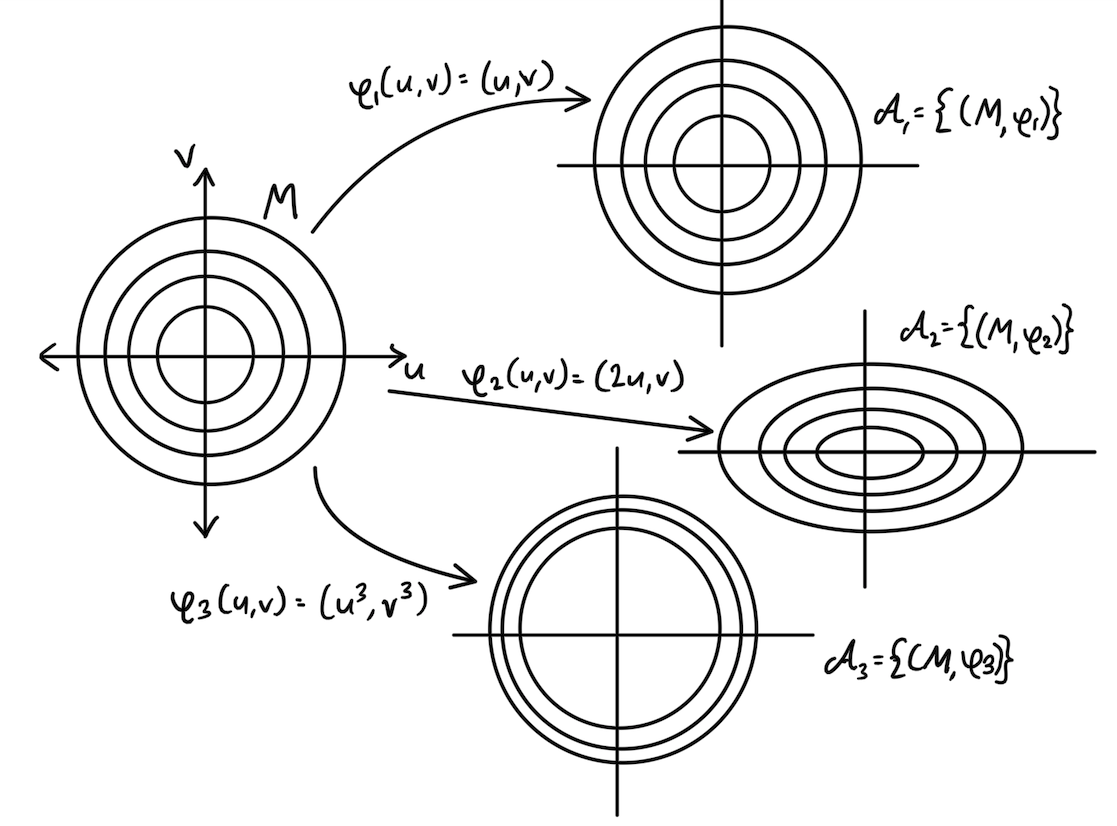
\includegraphics[scale=0.32]{img/Different_Atlases.PNG}
    \end{center}

    In the visual above, notice that

    \begin{enumerate}
      \item $\mathcal{A}_1, \mathcal{A}_2, \mathcal{A}_3$ are all smooth atlases (trivially).
      \item $\varphi_1$ and $\varphi_2$ are smoothly compatible $\implies \mathcal{A}_{12} = \{(M, \varphi_1), (M, \varphi_2)\}$ is a smooth atlas. 
      \item $\varphi_3$ is not smoothly compatible with either $\varphi_1$ nor $\varphi_2$. This implies that $\mathcal{A}_{13} = \{(M, \varphi_1), (M, \varphi_3)\}, A_{23} = \{(M, \varphi_2), (M, \varphi_3)\}$ are not smooth atlases.
    \end{enumerate}

    Clearly, $\varphi_1$ and $\varphi_2$ are closely related as they are smoothly compatible. Furthermore, 

      \begin{equation}
        \mathcal{A}_1 \subset \mathcal{A}_{12}, \;\;\; \mathcal{A}_2 \subset \mathcal{A}_{12}
      \end{equation}

    Now, imagine an atlas that contains $(M, \varphi_1), (M,\varphi_2)$, and all other possible charts that are smoothly compatible with $\varphi_1$ and $\varphi_2$. This creates a "maximal" smooth atlas. 

    \begin{definition}[Maximal Smooth Atlas]
      \label{def:maximal-smooth-atlas}
      A \textit{maximal smooth ($C^k$)atlas} is a smooth ($C^k$) atlas that is not contained in any strictly larger smooth atlas. In other words, it is the largest possible atlas in which every chart is smoothly ($C^k$) compatible with one another. 
    \end{definition}

    The existence of this maximal smooth ($C^k$) atlas wouldn't be as helpful without the following lemma, which allows us to easily describe it. 

    \begin{lemma}[Induced Maximal Smooth Atlases of Topological Manifolds]
      \label{thm:induced-maximal-smooth-atlases-of-topological}
      Let $M$ be a topological $n$-manifold. 
      \begin{enumerate}
        \item Every smooth atlas for $M$ is contained in a unique \hyperref[def:maximal-smooth-atlas]{maximal smooth atlas}. 
        \item Two smooth atlases for $M$ determine the same maximal smooth atlas if and only if their union is a smooth atlas. 
      \end{enumerate}
      That is, let $A_1, \ldots, A_a, B_1, \ldots, B_b, C_1, \ldots, C_c$ be a collection of smooth atlases on $M$ such that any union of the $A_i$'s, any union of the $B_i$'s, and any union of the $C_i$'s, are smooth atlases. Then, we can imagine all of the $A_i$'s as subsets of the unique maximal atlas $A^*$, all of the $B_i$'s as subsets of the unique maximal atlas $B^*$, and all of the $C_i$'s as subsets of the unique maximal atlas $C^*$. 
      \begin{center}
        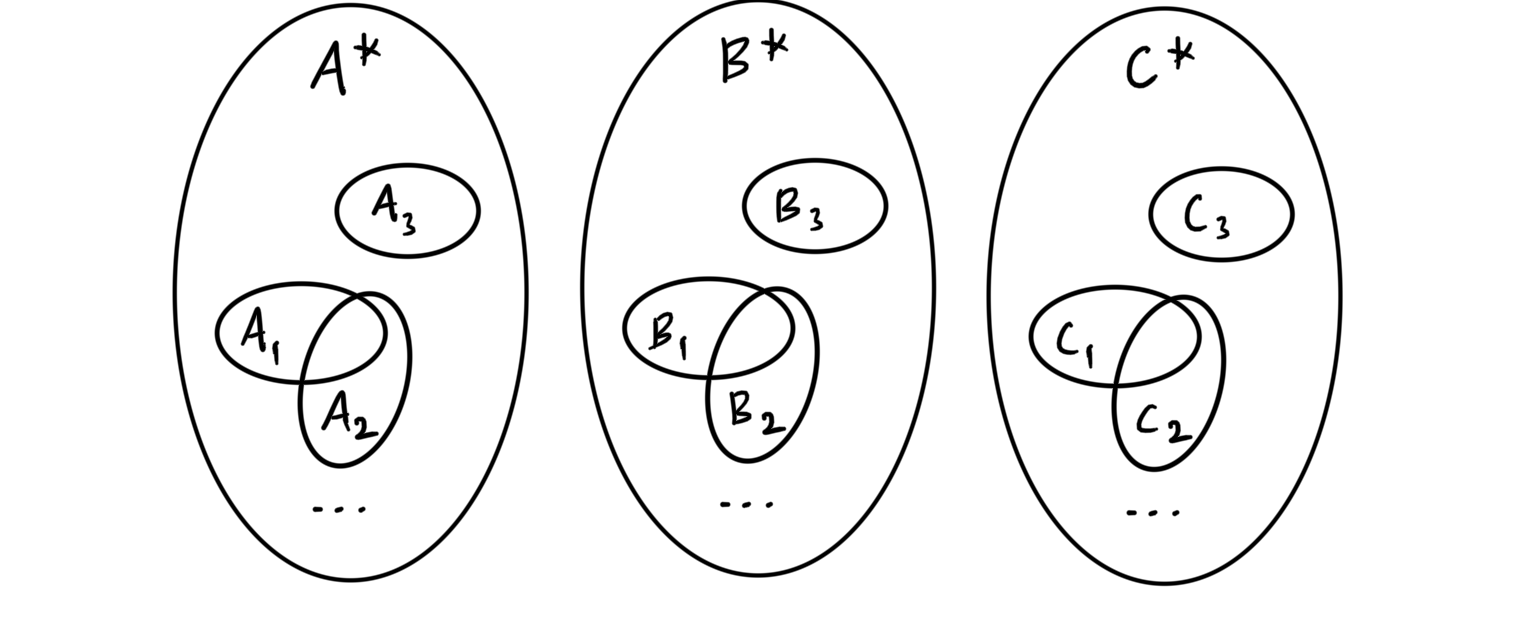
\includegraphics[scale=0.25]{img/Maximal_Smooth_Atlas_Classes.PNG}
      \end{center}
      Therefore, there can exist many smooth structures for topological manifold $M$. 
    \end{lemma}

    From the lemma, we can clearly see that the atlases form an equivalence class, one for smooth structure. 

    \begin{definition}[Smooth Equivalence Relation]
      \label{def:smooth-equivalence-relation}
      Two atlases $A_1, A_2$ are \textit{smoothly ($C^k$) equivalent} if $A_1 \cup A_2$ forms a smooth ($C^k$) atlas. Note that $C^k$-equivalence is a relation, and so the collection of all atlases that are $C^k$-equivalent forms a $C^k$-equivalence class, which is actually detremined uniquely by the maximal atlas. 
    \end{definition}

    \begin{definition}[Smooth ($C^k$) Structure, Smooth ($C^k$) Manifolds]
      \label{def:smooth-ck-structure-smooth-ck-manifolds}
      Three closely related definitions: 
      \begin{enumerate}
        \item A \textit{smooth ($C^k$) structure} on a topological $n$-manifold $M$ is a maximal smooth ($C^k$) atlas.
        \item A \textit{smooth ($C^k$) manifold} is a pair $(M, \mathcal{A})$, $M$ being a topological manifold and $\mathcal{A}$ a smooth ($C^k$) structure. 
        \item A chart, or a coordinate map, of a smooth manifold, is called a \textit{smooth chart}. 
      \end{enumerate}
    \end{definition}

    Three final things to mention:
    \begin{enumerate}
      \item There exist topological manifolds that admit no smooth structures at all. So, we cannot add a smooth structure to every topological manifold. 

      \item It is generally not convenient to define a smooth structure by explicitly describing a \hyperref[def:maximal-smooth-atlas]{maximal smooth atlas}, since such an atlas contains many charts. Fortunately, by the previous lemma, we only need to specify \textit{some} smooth atlas, which will induce a maximal smooth atlas. 

      \begin{align*}
          \text{Specify } A_i & \implies \text{Smooth Structure} = A^*\\
          \text{Specify } B_i & \implies \text{Smooth Structure} = B^*\\
          \text{Specify } C_i & \implies \text{Smooth Structure} = C^*
      \end{align*}

      \item In many cases, one proves that a topological manifold $M$ has a smooth atlas by directly computing and seeing that $\psi \circ \varphi^{-1}$ is smooth, for every pair $\psi, \varphi$ in the atlas. Clearly, all of the $\psi \circ \varphi^{-1}$ are \hyperref[pst-def:homeomorphism]{homeomorphisms} (as compositions of homeomorphisms), and since we've proved them to be smooth, it automatically follows that they are \hyperref[def:diffeomorphism]{diffeomorphisms}. j
    \end{enumerate}

    \begin{definition}[Other Classes of Manifolds]
      \label{def:other-classes-of-manifolds}
 Let $M$ be a manifold. 
      \begin{enumerate}
        \item A $C^0$ manifold is just a topological manifold. 
        \item If the transition mappings of $M$ can be expressed as real analytic (i.e. expressible as a convergent power series in a neighborhood of each point), then $M$ is said to have a $C^\omega$ structure, making $M$ a \textit{real-analytic manifold}. 
        \item If $M$ has an even dimension $2m$, then we can use the fact that $\mathbb{R}^{2m} \simeq \mathbb{C}^m$ to define a $C^m$ structure, making $M$ a \textit{complex manifold}. 
      \end{enumerate}
    \end{definition}

    \begin{example}[Two Incompatible Smooth Structures on $\mathbb{R}$]
      \label{ex:two-incompatible-smooth-structures-on-r}
      Consider $\mathbb{R}$ with the charts $(\mathbb{R}, \text{id})$ and $(\mathbb{R}, x^3)$. Each of these charts cover $\mathbb{R}$, but they are not $C^\infty$-compatible (since $\sqrt[3]{x}$ is not $C^\infty$), which means that they generate different maximal atlases. In fact, in $\mathbb{R}$, there are an infinitely many non-compatible maximal atlases each giving the topological space $\mathbb{R}$ the structure of a differentiable manifold. 
    \end{example}

    We can actually prove a stronger theorem. 

    \begin{theorem}[Distinct Smooth Structures on Positive-Dimensional Smooth Manifolds]
      \label{thm:distinct-smooth-structures-on-positive}
      Let $M$ be a nonempty topological manifold of dimension $n \geq 1$. If $M$ has a smooth structure, then it has uncountably many distinct ones. 
    \end{theorem}

    \subsubsection{Local Coordinate Representations}

      We describe how one usually thinks about coordinate charts on a smooth manifold. Once we shoose a smooth chart $(U, \varphi)$ on $M$, the coordinate map 

        \begin{equation}
          \varphi: U \longrightarrow \Tilde{U} \subset \mathbb{R}^n
        \end{equation}

      can be thought of as giving an \textit{identification} between $U$ and $\Tilde{U}$. Using this identification, we can think of $U$ simultaneously as an open subset of $M$ and as an open subset of $\mathbb{R}^n$. You can visualize this identification by thinking of a "grid" drawn on $U$ representing the inverse images of the coordinate lines under $\varphi$. 

      \begin{center}
        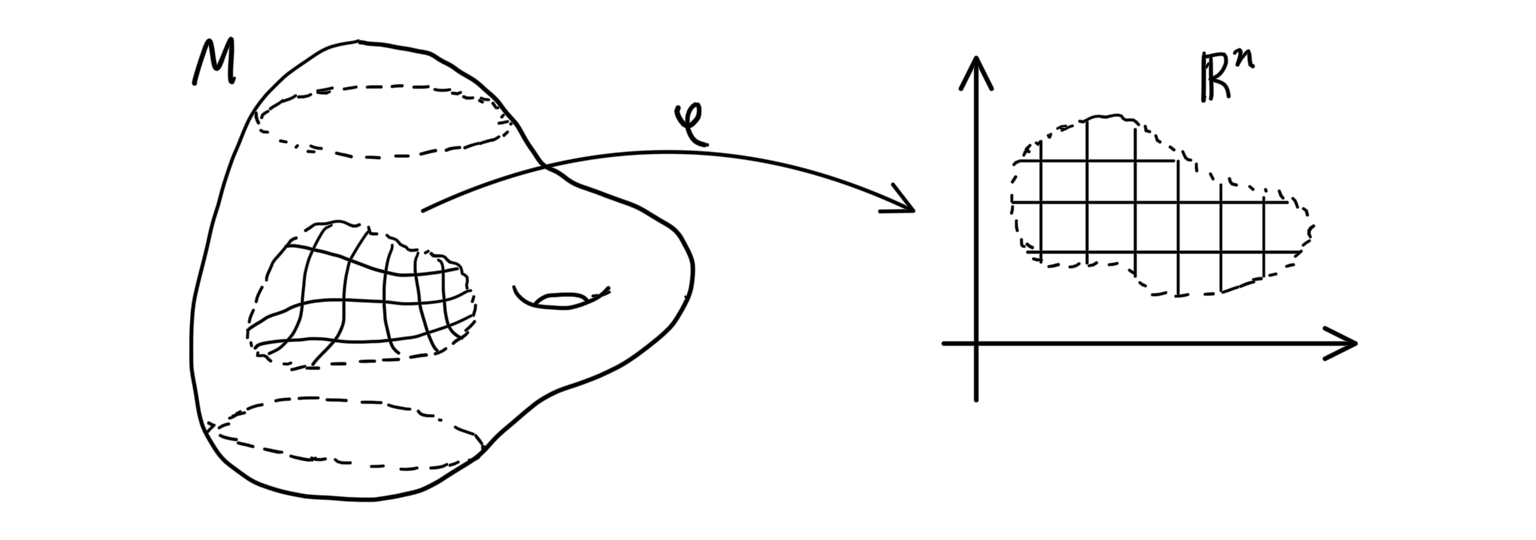
\includegraphics[scale=0.25]{img/Grid_Identification.PNG}
      \end{center}

      Using this identification, we can represent point $p \in U$ by its coordinates

        \begin{equation}
          \big( x^1, x^2, ..., x^n \big) = \varphi(p)
        \end{equation}

      and think of this $n$-tuple as \textit{being} the point $p$ (even though $p$, as an abstract point, really has no coordinates). This is typically expressed by saying that $\big( x^1, ..., x^n\big)$ is the (local) coordinate representation for $p$" or "$p = \big( x^1, ..., x^n\big)$ in local coordinates." Note that the curves (lines) do not necessarily have to be rectilinear. The projected lines from Euclidean space onto the manifold can be of any shape, including polar, as long as it is a \hyperref[pst-def:homeomorphism]{homeomorphism}. 

      \begin{definition}[Einstein Summation Notation]
        \label{def:einstein-summation-notation}
        Due to the abundance of summations in this chapter, we will abbreviate such a sum as such 
          \begin{equation}
            \sum_i x^i E_i = x^i E_i
          \end{equation}
      \end{definition}

    \subsubsection{Construction of a Smooth Manifold}

      When defining a smooth manifold, we start with a topological space and check that it is a topological manifold, and then we specify a smooth structure. The following lemma combines these steps into one. 

      \begin{lemma}[Smooth Manifold Construction Lemma]
        \label{thm:smooth-manifold-construction-lemma}
        Let $M$ be a set, and suppose we are given a collection $\{U_\alpha\}$ of subsets of $M$, together with an injective map $\varphi_\alpha: U_\alpha \longrightarrow \mathbb{R}^n$ for each $\alpha$, such that the following properties are satisfied:
        \begin{enumerate}
          \item For each $\alpha$, $\varphi_\alpha (U_\alpha)$ is an open subset of $\mathbb{R}^n$.
          \item For each $\alpha$ and $\beta$, $\varphi_\alpha (U_\alpha \cap U_\beta)$ and $\varphi_\beta (U_\alpha \cap U_\beta)$ are open in $\mathbb{R}^n$. 
          \item Whenever $U_\alpha \cap U_\beta \neq \emptyset$, $\varphi_\alpha \circ \varphi_\beta^{-1}: \varphi_\beta (U_\alpha \cap U_\beta) \longrightarrow \varphi_\alpha (U_\alpha \cap U_\beta)$ is a \hyperref[def:diffeomorphism]{diffeomorphism}. 
          \item $M$ is second countable. 
          \item $M$ is Hausdorff. 
        \end{enumerate}
        Then, $M$ has a unique smooth manifold structure such that each $(U_\alpha, \varphi_\alpha)$ is a smooth chart. 
      \end{lemma}

  \subsection{Manifolds with Boundaries}

    We may come across manifolds which have a "boundary" of some sort, such as the closed unit ball in $\mathbb{R}^n$ and the closed upper hemisphere in $S^n$. 

    \begin{definition}[Euclidean Upper Half-Space]
      \label{def:euclidean-upper-half-space}
      The \textit{closed $n$-dimensional upper half-space} $\mathbb{H}^n \subset \mathbb{R}^n$ is defined

        \begin{equation}
          \mathbb{H}^n \equiv \big\{ (x^1, x^2, ..., x^n) \in \mathbb{R}^n \;|\; x^n \geq 0\big\}
        \end{equation}

      $\mathbb{H}^2$ and $\mathbb{H}^3$ are shown below. 

      \begin{center}
        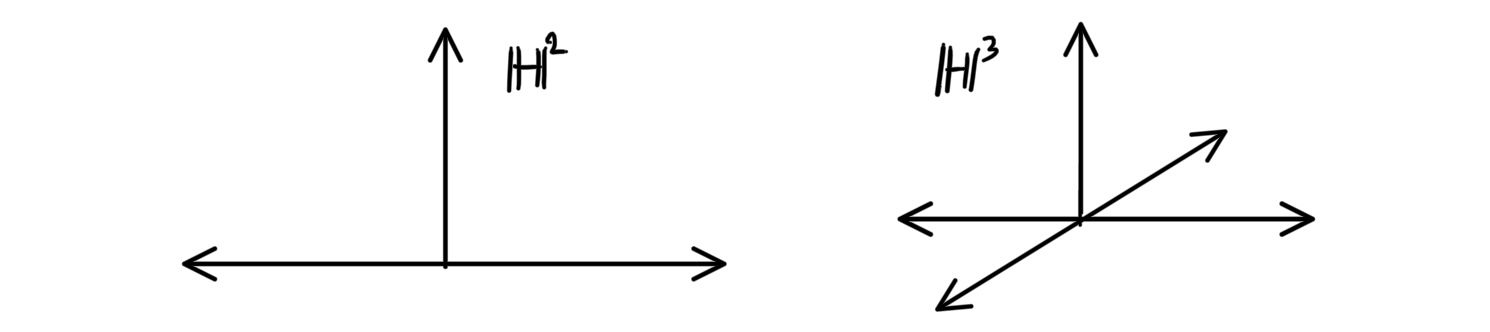
\includegraphics[scale=0.25]{img/Half_Euclidean_Space.PNG}
      \end{center}

      Clearly, $\mathbb{H}^n$ has the \hyperref[pst-def:subspace-topology]{subspace topology} induced by that of $\mathbb{R}^n$, allowing charts to map open neighborhoods of boundary points. We also define

      \begin{align*}
        \Int(\mathbb{H}^n) \equiv \big\{ (x^1, x^2, ..., x^n) \in \mathbb{R}^n \;|\; x^n > 0\big\} \\
        \partial(\mathbb{H}^n) \equiv \big\{ (x^1, x^2, ..., x^n) \in \mathbb{R}^n \;|\; x^n = 0\big\}
      \end{align*}
    \end{definition}

    \begin{definition}[Smooth Maps between Subsets]
      \label{def:smooth-maps-between-subsets}
      Note that a smooth map from an arbitrary subset $A \subset \mathbb{R}^n$ to $\mathbb{R}^k$ is defined to be a map that admits a smooth extension to an open neighborhood of each point. 
      \begin{center}
        % \includegraphics[]{}
      \end{center}
    \end{definition}

    \begin{definition}[Topological Manifold with Boundary]
      \label{def:topological-manifold-with-boundary}
      An \textit{$n$-dimensional topological manifold with boundary} is a second-countable \hyperref[pst-def:hausdorff-space]{Hausdorff space} $M$ that is \hyperref[pst-def:locally-homeomorphic]{locally homeomorphic} to $\mathbb{H}^n$. An open subset $U \subset M$ together with a \hyperref[pst-def:homeomorphism]{homeomorphism} $\varphi$ from $U$ to an open subset of $\mathbb{H}^n$ is called a chart.

      \begin{enumerate}
        \item $(U, \varphi)$ is an \textit{interior chart} if $\varphi(U) \subset \Int(\mathbb{H}^n)$. 
        \item $(U, \varphi)$ is a \textit{boundary chart} if $\varphi(U) \cap \partial \mathbb{H}^n \neq \emptyset$
      \end{enumerate}

      \begin{center}
        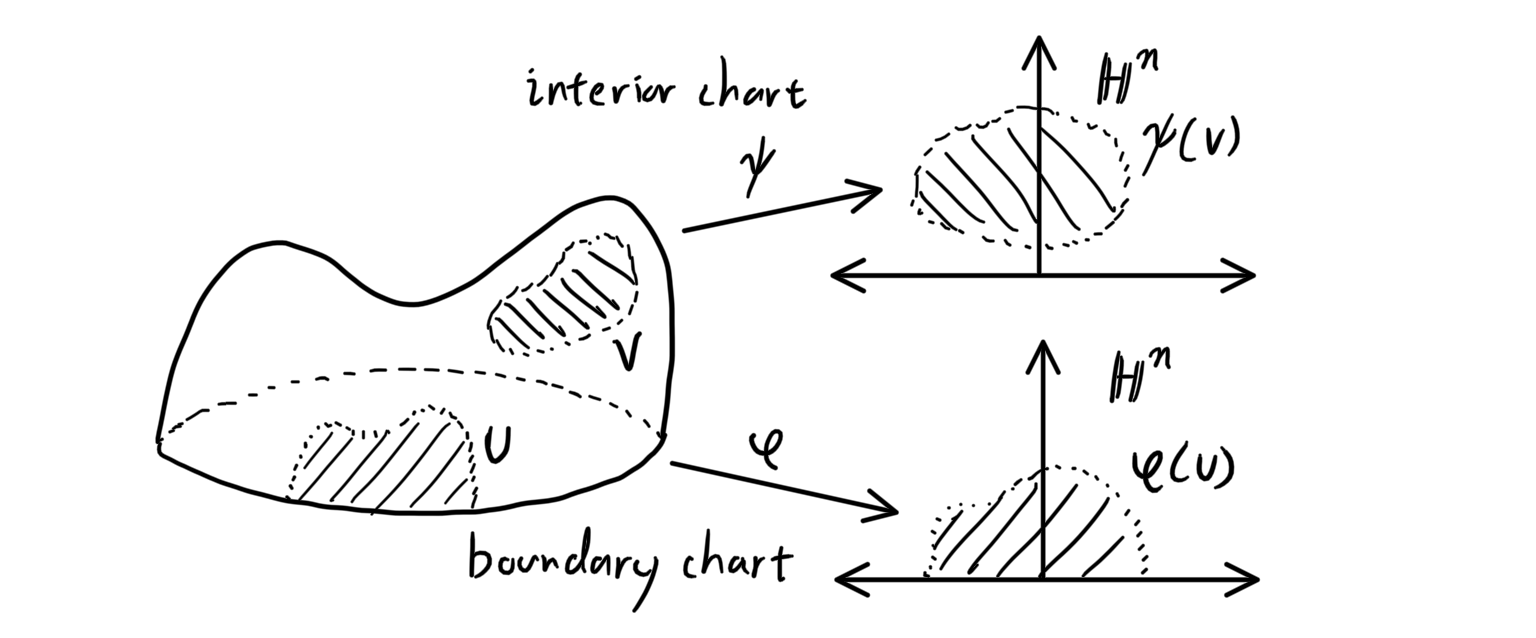
\includegraphics[scale=0.25]{img/Interior_Boundary_Chart.PNG}
      \end{center}

      A point $p \in M$ is a \textit{boundary point} if its image under some smooth shart is in $\partial \mathbb{H}^n$; the set of all such boundary points is denoted $\partial M$. The set of all interior points of $M$ is denoted Int$(M)$. Furthermore, it turns out that

        \begin{equation}
          M = \text{Int}(M) \sqcup \partial M
        \end{equation}

      That is, $M$ can be partitioned into its interior and boundary. 
    \end{definition}

    To define a smooth structure on a manifold with boundary, we must be able to define smooth maps that encompasses cases between boundary charts. 

    \begin{definition}[Smooth Maps on Open Subsets of the Half-Space]
      \label{def:smooth-maps-on-open-subsets-of-the-half-space}
      Let $U$ be an open subset of $\mathbb{H}^n$. A map $F: U \longrightarrow \mathbb{R}^k$ is \textbf{smooth} if for each $x \in U$ there exists an open neighborhood $V \subset \mathbb{R}^n$ of $x$ and a smooth map (extension) $\Tilde{F}: V \longrightarrow \mathbb{R}^k$ that agrees with $F$ on $V \cap \mathbb{H}^n$. 
    \end{definition}

    \begin{definition}[Smooth Manifold with Boundary]
      \label{def:smooth-manifold-with-boundary}
      Let $M$ be a \hyperref[def:topological-manifold-with-boundary]{topological manifold with boundary}. A \textit{smooth structure} for $M$ is defined to be a \hyperref[def:maximal-smooth-atlas]{maximal smooth atlas}, i.e. a collection of charts whose domains cover $M$ and whose transition maps (and inverses) are smooth as in it admits smooth extensions. With such a structure, $M$ is called a \textit{smooth manifold with boundary}. 
    \end{definition}

    Note that the boundary of manifold $M$ and the boundary of $M$ as a subset of a bigger topological space are two completely different sets. 

    \begin{example}[The Closed Unit Disk as a Manifold with Boundary]
      \label{ex:the-closed-unit-disk-as-a-manifold-with-boundary}
      Let $B^2$ be the open unit disk in $\mathbb{R}^2$. Then, $\bar{B^2}$, the closed unit disk, is a \hyperref[def:smooth-manifold-with-boundary]{smooth manifold with boundary}, with the boundary being the circle $S^1$. However, if we interpret $B^2$ as a topological subspace 
      \begin{enumerate}
        \item $\mathbb{R}^2$, the topological boundary is $S^1$. 
        \item $\mathbb{R}^3$, the topological boundary is $\bar{B^2}$. 
        \item $\bar{B^2}$, the topological boundary is $\emptyset$. 
      \end{enumerate}
    \end{example}

    Furthermore, every smooth $n$-manifold can be considered a smooth $n$-manifold with boundary by composing each chart mapping with a \hyperref[def:diffeomorphism]{diffeomorphism} from $\mathbb{R}^n$ to $\mathbb{H}^n$ such as

      \begin{equation}
        \big(x^1, ..., x^{n-1}, x^n \big) \mapsto \big( x^1, ..., x^{n-1}, e^{x^n} \big)
      \end{equation}

    This modifies all manifold charts to take its values in $\Int(\mathbb{H}^n)$ without affecting the smooth compatibility condition. 
    Also, given a smooth $n$-manifold with boundary $M$, $\Int(M)$ is also a topological $n$-manifold since the subfamily of all smooth interior charts is also a smooth atlas. 

\section{Smooth Maps}

  \begin{definition}[Smooth Maps from Manifolds to Euclidean Space]
    \label{def:smooth-maps-from-manifolds-to-euclidean-space}
    If $M$ is a smooth $n$-manifold, a function $f: M \longrightarrow \mathbb{R}^k$ is said to be \textit{smooth} if for every $p \in M$, there exists a smooth chart $(U, \varphi)$ for $M$ whose domain contains $p$ and such that the composite function, called the \textit{coordinate representation of $f$}
    \begin{equation}
      \hat{f} = f \circ \varphi^{-1}: \varphi(U) \subset \mathbb{R}^n \longrightarrow \mathbb{R}^k
    \end{equation}
    is smooth. 
    \begin{center}
      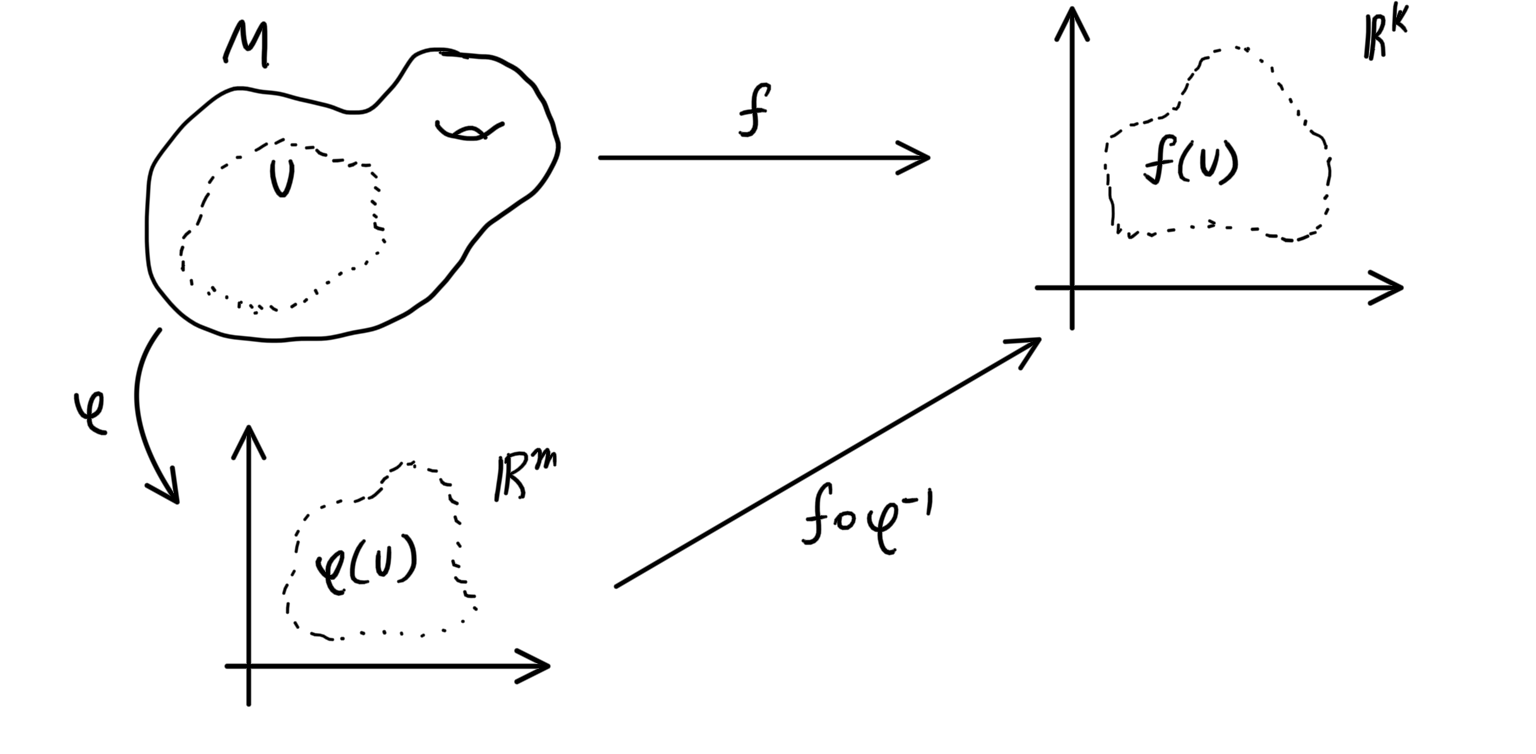
\includegraphics[scale=0.24]{img/Function_Manifold_to_Euclidean_Space.PNG}
    \end{center}
    By definition, $f$ is smooth if and only if its coordinate representation is smooth in some smooth chart around every point. 
  \end{definition}

  The set of smooth real-valued functions $f: M \longrightarrow \mathbb{R}$ is denoted as $C^\infty (M)$. Since sums and constant multiples of smooth functions are smooth, $C^\infty (M)$ is a \hyperref[lin-def:vector-space]{vector space}. 

  \begin{definition}[Smooth Maps between Manifolds]
    \label{def:smooth-maps-between-manifolds}
    Let $M, N$ be smooth $m, n$-manifolds, and let $F: M \longrightarrow N$ be any map. Then, $F$ is a \textit{smooth map} if for every $p \in M$, there exist smooth charts $(U, \varphi)$ containing $p$ and $(V, \psi)$ containing $F(p)$ such that $F(U) \subset V$ and the composite map 

      \begin{equation}
        \psi \circ F \circ \varphi^{-1}: \varphi(U) \subset \mathbb{R}^m \longrightarrow \psi(V) \subset \mathbb{R}^n
      \end{equation}

    is smooth (in the regular Euclidean sense). The abstraction of $F$ does not do us much good computation wise, so more often than not, we look at the \textit{coordinate representation of $F$}

      \begin{equation}
        \hat{F} \equiv \psi \circ F \circ \varphi^{-1}
      \end{equation}

    In here, $\hat{F}$ is really just a representation of the abstract map $F$ in specific local coordinates determined by $\varphi$ and $\psi$. Once $\varphi, \psi$ are determined, we can often ignore the distinction between $F$ and $\hat{F}$. 

    Application-wise, there are three ways to prove that a particular map is smooth: 
    \begin{enumerate}
      \item Write the map in smooth local coordinates and recognize its component functions as compositions of smooth elementary functions. 
      \item Exhibit the map as a composition of known smooth maps. 
      \item Use some special-purpose theorem that applies to the particular case. 
    \end{enumerate}

    \begin{center}
      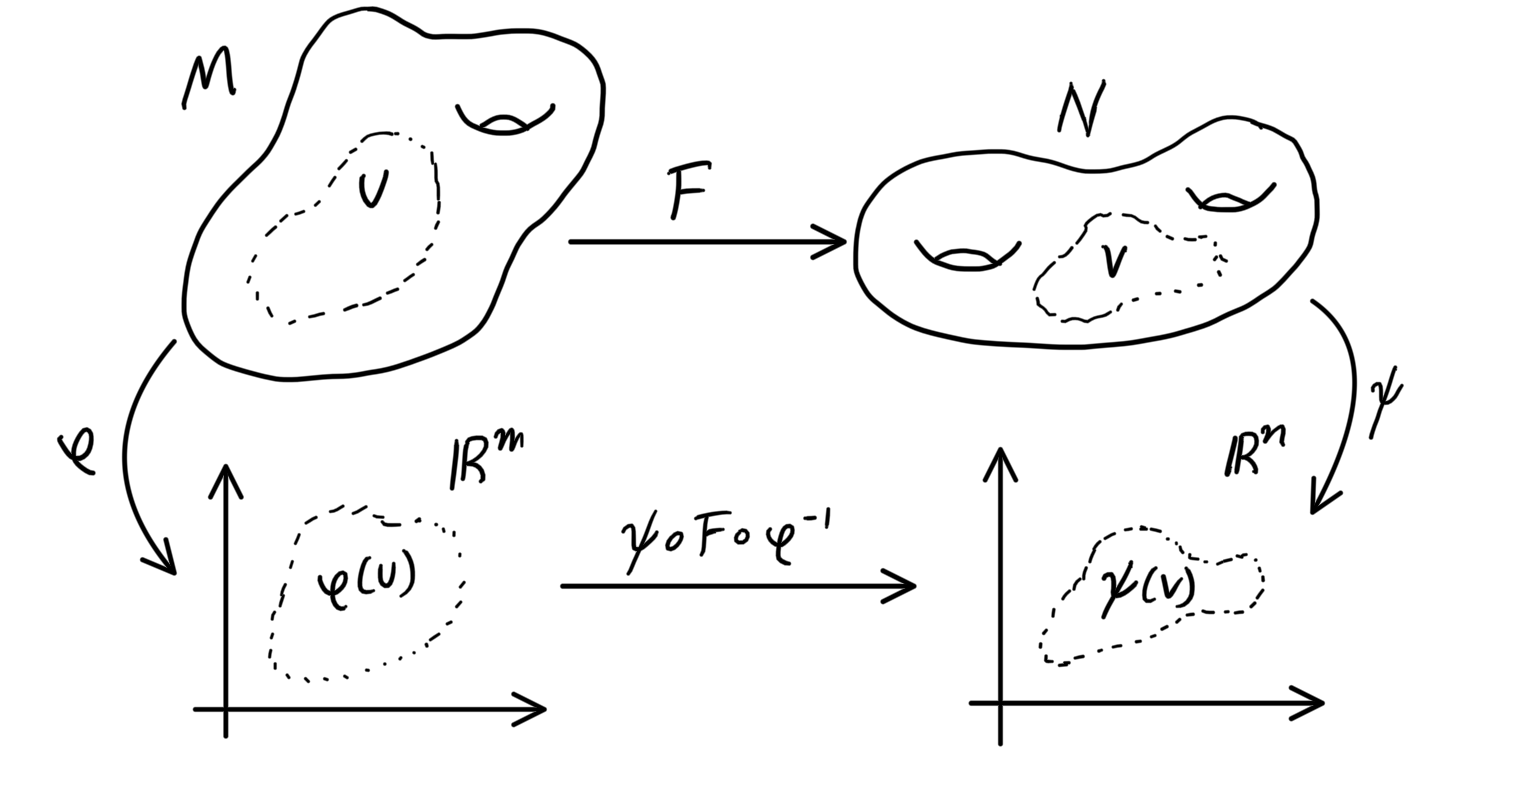
\includegraphics[scale=0.25]{img/Functions_between_Manifolds.PNG}
    \end{center}
  \end{definition}

  \begin{theorem}[Properties of Smooth Maps between Manifolds]
    \label{thm:properties-of-smooth-maps-between-manifolds}
    Given $M, N$ smooth $m, n$-manifolds, with arbitrary map $F: M \longrightarrow N$, we have the following properties: 

    \begin{enumerate}
      \item If $F$ is smooth, then $F$ is continuous. 
      \item The composition of smooth maps between smooth manifolds is smooth. 
      \item If there exists an open cover $\{U_\alpha\}_\alpha$ of $M$ and smooth maps $F_\alpha: U_\alpha \longrightarrow N$ such that they agree on overlaps
        \begin{equation}
          F_\alpha \big|_{U_\alpha \cap U_\beta} = F_\beta \big|_{U_\alpha \cap U_\beta} \text{ for all } \alpha, \beta
        \end{equation}
      then there exists a unique smooth map $F: M \longrightarrow N$ such that $F$ agrees with all the $F_\alpha$'s. 
    \end{enumerate}

    The last property is convenient for when we wish to construct a global smooth map from local ones. 
  \end{theorem}

  \begin{proof}
    We prove the first two properties: 
    \begin{enumerate}
      \item Suppose $F: M \longrightarrow N$ is smooth. The definition of smoothness guarantees that for every $p \in M$, we can choose smooth charts $(U, \varphi)$ containing $p$ and $(V, \psi)$ containing $F(p)$ such that $F(U) \subset V$ and $\psi \circ F \circ \varphi^{-1}: \psi(U) \longrightarrow \varphi(V)$ is smooth, hence continuous. Since $\varphi$ and $\psi$ are \hyperref[pst-def:homeomorphism]{homeomorphisms}, this implies that

      \begin{equation}
        F \big|_U = \psi^{-1} \circ \big( \psi \circ F \circ \varphi^{-1} \big) \circ \varphi : U \longrightarrow V
      \end{equation}

      is continuous, as a composition of continuous maps. Since $F$ is continuous at each point, it is continuous on $M$.

      \item Looking at the diagram below, we can see that since $F, G$ are smooth, the mappings (between Euclidean spaces) $\theta \circ F \circ \varphi^{-1}$ and $\psi \circ G \circ \theta^{-1}$ are smooth, meaning that their composition

        \begin{equation}
          (\psi \circ G \circ \theta^{-1}) \circ (\theta \circ F \circ \varphi^{-1}) = \psi \circ (G \circ F) \circ \varphi^{-1}
        \end{equation}

      is smooth. By definition, this means that $G \circ F$ is smooth. 

      \begin{center}
        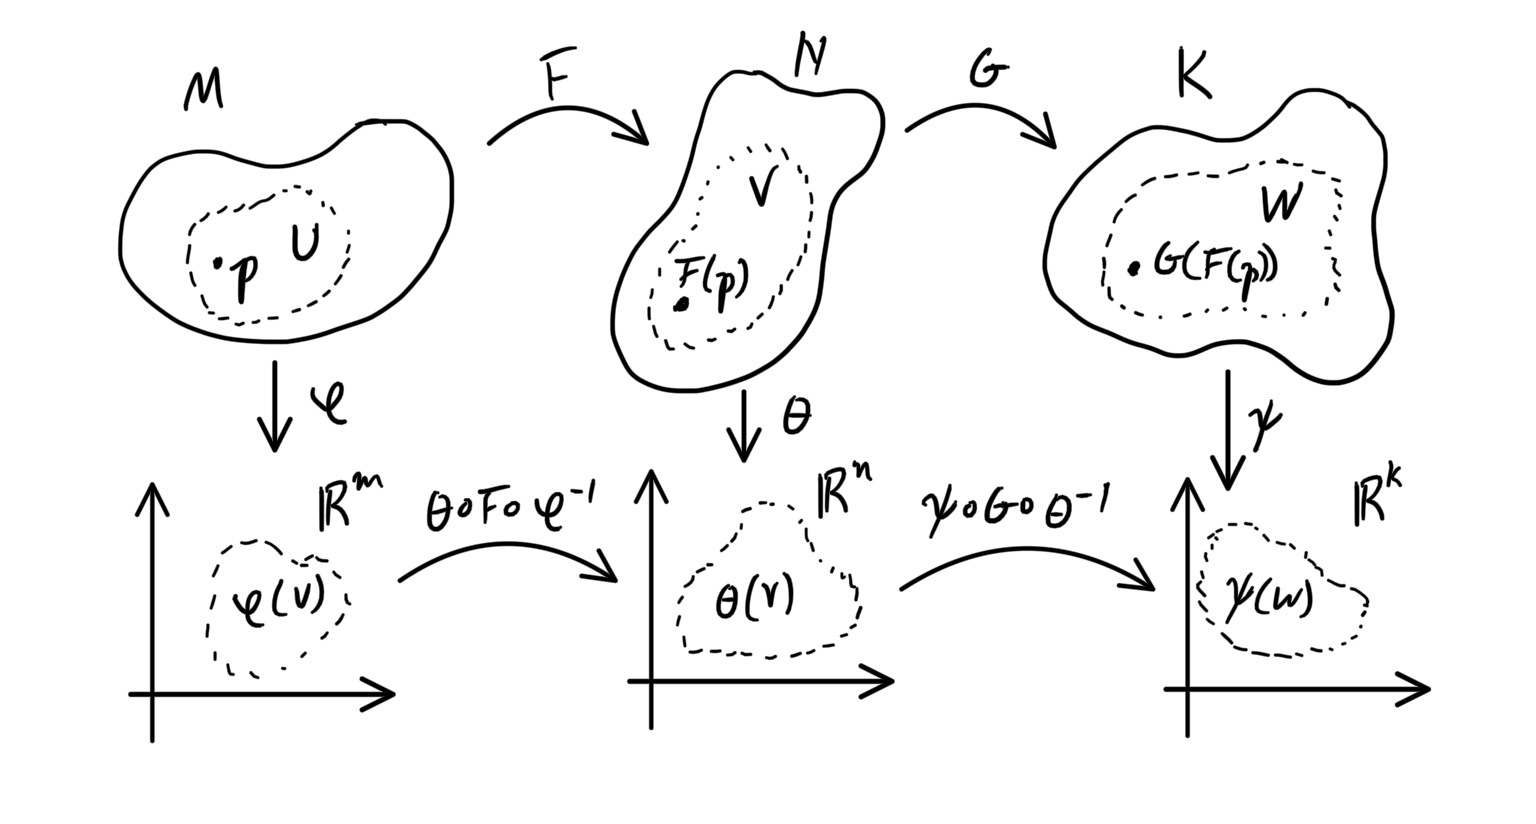
\includegraphics[scale=0.25]{img/Composition_of_Smooth_Manifold_Mappings.PNG}
      \end{center}

    \end{enumerate}
  \end{proof}

  \subsection{Clarification of Multiple Meanings of Smoothness}

    We emphasize that the smoothness of a map $F$ between manifolds depends \textbf{only} on the smoothness of its coordinate representation $\hat{F}$! This warning is more clearly explained through the following example. 

    \begin{example}[Mappings between Lines with Different Smooth Structures]
      \label{ex:mappings-between-lines-with-different-smooth}
      Let us have manifold $\mathbb{R}$ with the standard smooth structure determined by global mapping id$: \mathbb{R} \longrightarrow \mathbb{R}$. Let us have a second manifold $\Tilde{\mathbb{R}}$ with smooth structure determined by global mapping $\psi(x) = x^{1/3}$. Now, let us have mappings (between manifolds) $F_1, F_2, F_3: \mathbb{R} \longrightarrow \Tilde{\mathbb{R}}$ where $F_1 (x) = x, F_2 (x) = x^3, F_3(x) = x^6$, as shown below. 

      \begin{center}
        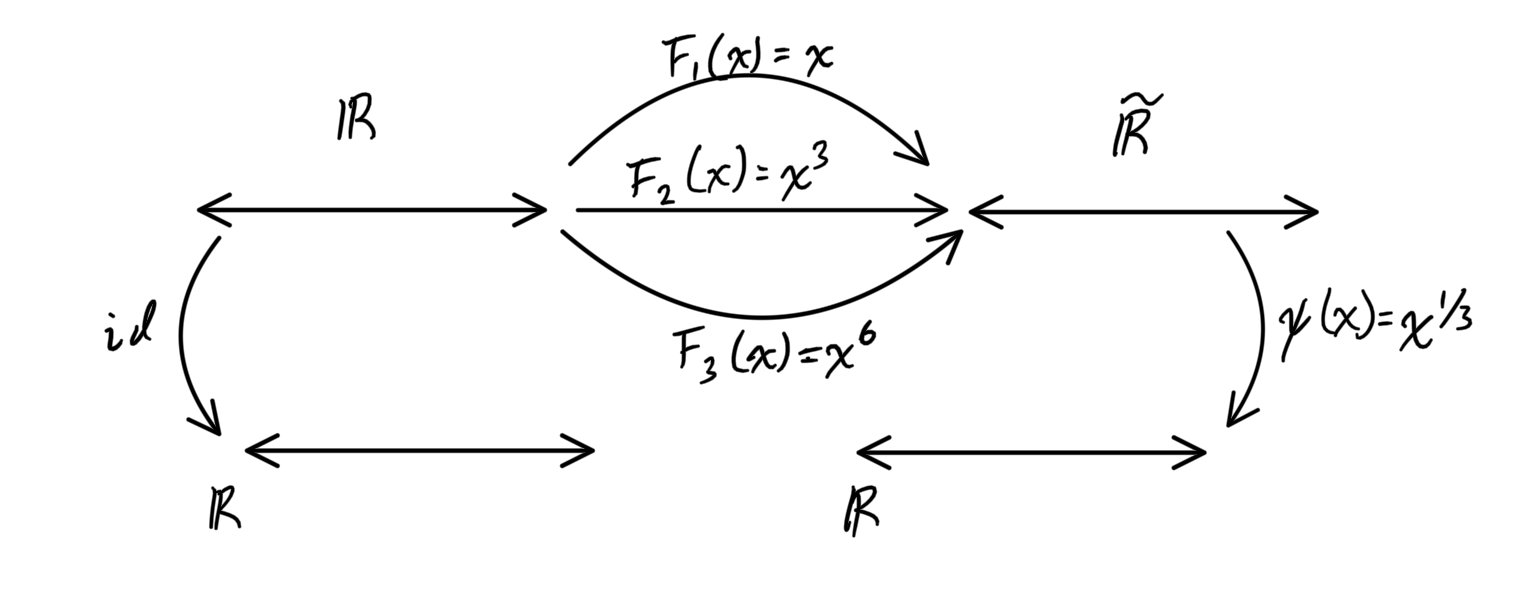
\includegraphics[scale=0.25]{img/Real_Line_Manifold_Functions.PNG}
      \end{center}

      Then,

      \begin{align*}
        \psi \circ F_1 \circ \text{id}^{-1} (x)= x^{1/3} & \implies F_1 \text{ not smooth} \\
        \psi \circ F_2 \circ \text{id}^{-1}(x) = x & \implies F_2 \text{ smooth} \\
        \psi \circ F_3 \circ \text{id}^{-1}(x) = x^{2} & \implies F_3 \text{ smooth} 
      \end{align*}
    \end{example}

    Note that the smoothness of the $F_i$'s when interpreting them as mappings between manifolds gives results compared to when we interpret them as regular mappings between Euclidean space. For example, $F_1$ is not smooth in the manifold sense even though it is clearly smooth in the Euclidean sense (since it is the identity mapping).  

  \subsection{Diffeomorphisms}

    \begin{definition}[Diffeomorphism]
      \label{def:diffeomorphism-2}
      A \textit{diffeomorphism} between smooth manifolds $M$ and $N$ is a smooth bijective map $F: M \longrightarrow N$ that has a smooth inverse. It is said that $M$ and $N$ are \textit{diffeomorphic} if there exists a diffeomorphism between them, denoted as 

        \begin{equation}
          M \approx N
        \end{equation}

      This is in fact an \hyperref[st-def:equivalence_relation]{equivalence relation}. Just as two topological spaces are considered to be the same if they are homeomorphic, two smooth manifolds are essentially indistinguishable if they are diffeomorphic. Clearly, diffeomorphisms preserve the dimensionalities of $M$ and $N$. 
    \end{definition}

    Clearly, if $M$ is any smooth manifold and $(U, \varphi)$ is a smooth coordinate chart on $M$, then $\varphi: U \longrightarrow \varphi(U) \subset \mathbb{R}^n$ is a \hyperref[def:diffeomorphism-2]{diffeomorphism} (by definition). 

    \begin{example}[Diffeomorphism from the Open Ball to $\mathbb{R}^n$]
      \label{ex:diffeomorphism-from-the-open-ball-to-rn}
      Let $B^n$ be the open unit ball in $\mathbb{R}^n$ (each with the standard smooth structure). Then, the map 

        \begin{equation}
          F: B^n \longrightarrow \mathbb{R}^n, \; F(x) \equiv \frac{x}{1 - \|x\|^2}
        \end{equation}

      is a diffeomorphism. 
    \end{example}

    \begin{example}[Mappings between Lines with Different Smooth Structures]
      \label{ex:mappings-between-lines-with-different-smooth-2}
      In the diagram below regarding a previous example, we have the three maps $F_1, F_2, F_3: \mathbb{R} \longrightarrow \Tilde{\mathbb{R}}$, where $\mathbb{R}$ is a smooth manifold with the standard smooth structure, and $\Tilde{\mathbb{R}}$ is a smooth manifold with the smooth structure consisting of $\psi$. 

      \begin{center}
        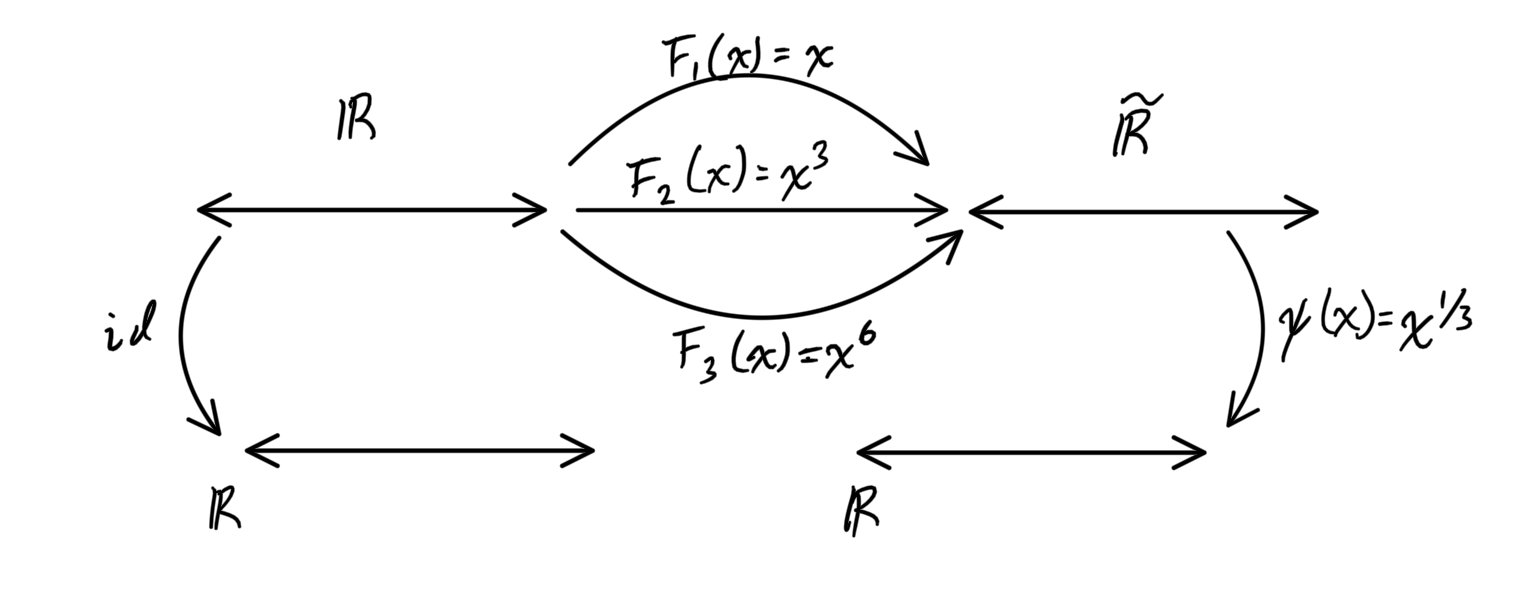
\includegraphics[scale=0.25]{img/Real_Line_Manifold_Functions.PNG}
      \end{center}

      To find out whether $F_i$ is a \hyperref[def:diffeomorphism-2]{diffeomorphism}, we must confirm that $F_i$ is bijective, smooth, and $F_i^{-1}$ is smooth. 

      \begin{enumerate}
        \item $F_1$ is clearly bijective. $\psi \circ F_1 \circ id^{-1} (x) = x^{1/3}$, so $F_1$ is not smooth. $id \circ F_1^{-1} \circ \psi^{-1} = x^3$, so $F_1^{-1}$ is smooth. 
        \item $F_2$ is clearly bijective. $\psi \circ F_2 \circ id^{-1} (x) = x$, so $F_2$ is smooth. $id \circ F_2^{-1} \circ \psi^{-1} = x$, so $F_2^{-1}$ is smooth.
        \item $F_3$ is not bijective. $\psi \circ F_3 \circ id^{-1} (x) = x^2$, so $F_3$ is smooth. Since $F_3$ is not injective, $F_3^{-1}$ is not well-defined. 
      \end{enumerate}

      Therefore, $F_2$ is the only diffeomorphism out of the three observed functions. 
    \end{example}

    \begin{definition}[Local Diffeomorphism]
      \label{def:local-diffeomorphism}
      $F: M \longrightarrow N$ is called a \textit{local diffeomorphism} if every point $p \in M$ has a neighborhood $U$ such that $F(U)$ is open in $N$ and 

        \begin{equation}
          F \big|_U : U \longrightarrow F(U)
        \end{equation}

      is a \hyperref[def:diffeomorphism-2]{diffeomorphism}. 
    \end{definition}

    \subsubsection{Nondiffeomorphic Smooth Structures on Manifolds}

      We already found out that there are many distinct structures on a positive-dimensional smooth manifold (in fact, an uncountable number of them). Furthermore, we have seen in this section that there may exist a \hyperref[def:diffeomorphism-2]{diffeomorphism} between the two copies of the topological manifold, each with distinct smooth structures ($F_2 (x) = x^3$ was a diffeomorphism between $(\mathbb{R}, \text{id})$ and $(\mathbb{R}, \psi)$. 

      This leads to the more interesting question of whether a given topological manifold admits smooth structures that are \textit{not} diffeomorphic to each other (as in, there exists no diffeomorphism $F$ between two copies of a given topological manifold, each with distinct smooth structures). 

      \begin{definition}[Diffeomorphic Smooth Structures]
        \label{def:diffeomorphic-smooth-structures}
        Given a topological manifold $M$, let $\mathcal{A}_1$ and $\mathcal{A}_2$ any two smooth structures on $M$. Then, 

          \begin{equation}
            (M, \mathcal{A}_1) \approx (M, \mathcal{A}_2)
          \end{equation}

        if there exists some \hyperref[def:diffeomorphism-2]{diffeomorphism} $F: (M, \mathcal{A}_1) \longrightarrow (M, \mathcal{A}_2)$. If the underlying manifold $M$ is known, then we write this more concisely as

          \begin{equation}
            \mathcal{A}_1 \approx \mathcal{A}_2
          \end{equation}

        and say that

        \begin{enumerate}
          \item $\mathcal{A}_1$ and $\mathcal{A}_2$ are diffeomorphic smooth structures on $M$, or
          \item $\mathcal{A}_1$ and $\mathcal{A}_2$ are identical smooth structures on $M$ up to diffeomorphism.
        \end{enumerate}

        In fact, the properties of smooth mappings imply that this relation $\approx$ endowed on the set of all smooth structures of $M$ forms equivalence classes of diffeomorphic smooth structures. Visually, given that $A^*, B^*, C^*, \ldots$ are smooth structures on $M$, they can be classified further into their respective diffeomorphism classes. 

        \begin{center}
          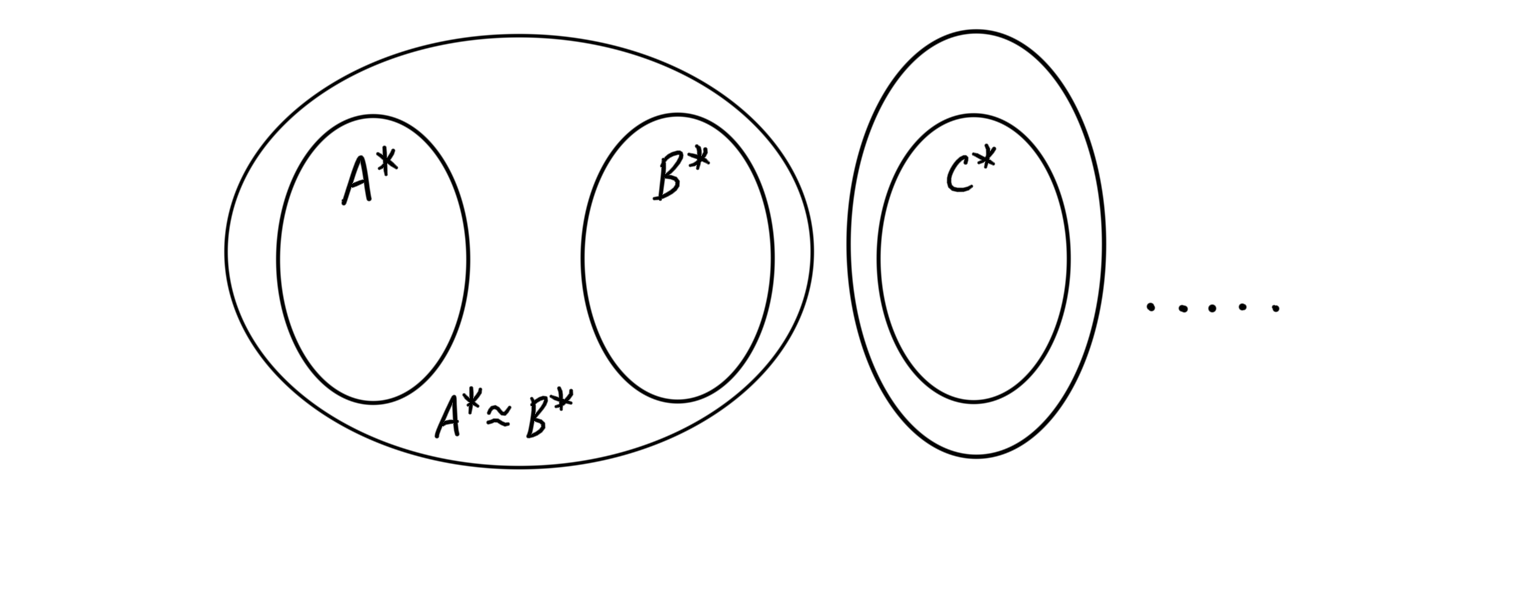
\includegraphics[scale=0.25]{img/Diffeomorphism_Classes.PNG}
        \end{center}
      \end{definition}

      \begin{example}[Diffeomorphic Smooth Structures of $\mathbb{R}$]
        \label{ex:diffeomorphic-smooth-structures-of-r}
        Since $F_2 = x^3$ is a \hyperref[def:diffeomorphism-2]{diffeomorphism} between $(\mathbb{R}, \text{id})$ and $(\Tilde{\mathbb{R}}, \psi)$, the two atlases $\{\mathbb{R}, \text{id}\}$ and $\{\mathbb{R}, \psi\}$ are diffeomorphic smooth structures: 

          \begin{equation}
            \{\mathbb{R}, \text{id}\} \approx \{\mathbb{R}, \psi\}
          \end{equation}

        It turns out that every smooth structure of $\mathbb{R}$ is equivalent in this sense. That is, there is only one smooth structure on $\mathbb{R}$ up to diffeomorphism. 
      \end{example}

      \begin{theorem}[Classification of Nondiffeomorphic Smooth Structures on $\mathbb{R}^n$]
        \label{thm:classification-of-nondiffeomorphic-smooth}
        The classification of smooth structures on Euclidean space is as follows: 
        \begin{enumerate}
          \item When $n \neq 4$, $\mathbb{R}^n$ has one unique smooth structure up to \hyperref[def:diffeomorphism-2]{diffeomorphism}.
          \item $\mathbb{R}^4$ has uncountably many distinct smooth structures, no two of which are diffeomorphic to each other! The study of \textit{exotic $\mathbb{R}^4$}s arises from this phenomenon. 
        \end{enumerate}
      \end{theorem}

      For compact manifolds, the situation is even more fascinating.

      \begin{theorem}[Classification of Nondiffeomorphic Smooth Structure on $\mathbb{S}^n$]
        \label{thm:classification-of-nondiffeomorphic-smooth-2}
        The table below details the number of unique smooth structures on $\mathbb{S}^n$ (for $n$ up to $12$) up to \hyperref[def:diffeomorphism-2]{diffeomorphism}. 

        \begin{center}
        \begin{tabular}{c|c|c|c|c|c|c|c|c|c|c|c|c}
          n & 1 & 2&3&4&5&6&7&8&9&10&11&12 \\
          \hline
          Smooth Struc. on $\mathbb{S}^n$ & 1&1&1&?&1&1&28&2&8&6&992&1
        \end{tabular}
        \end{center}

        Notice that the number of smooth structures on the exotic $4$-sphere is still unanswered. 
      \end{theorem}

  \subsection{Lie Groups}

    \begin{definition}[Lie Group]
      \label{def:lie-group}
    A \textit{Lie group} is a smooth manifold $G$ that is also a group in the algebraic sense, with the property that 

    \begin{enumerate}
      \item the multiplication map $m: G \times G \longrightarrow G, \;\; m(g, h) \equiv g h$ is smooth. That is, the function $\phi \circ m \circ (\varphi \times \psi)^{-1}: \mathbb{R}^{2m} \longrightarrow \mathbb{R}^m$ in the visual below is smooth in the Euclidean sense.  

      \begin{center}
        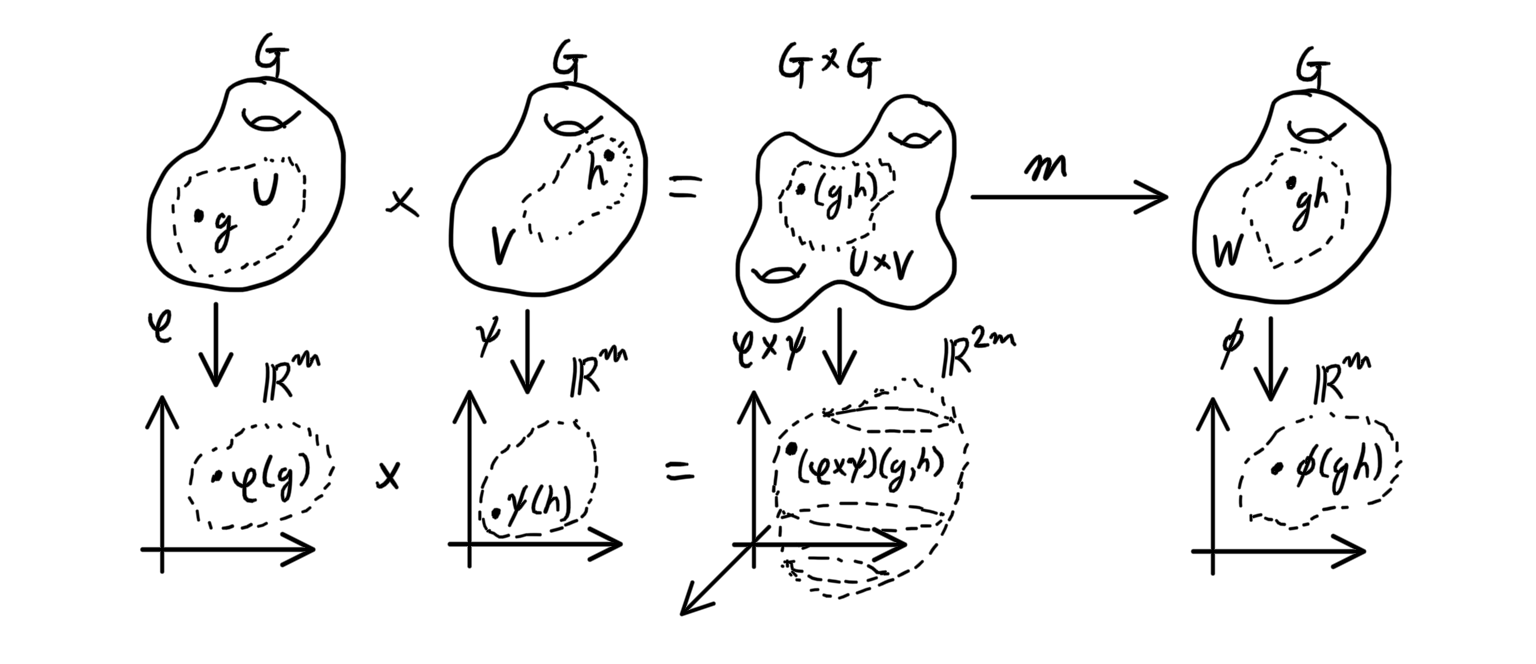
\includegraphics[scale=0.25]{img/Lie_Group_Multiplication.PNG}
      \end{center}

      \item the inversion map $i: G \longrightarrow G, \;\; i(g) \equiv g^{-1}$ is smooth. That is, the function $\theta \circ i \circ \varphi^{-1}: \mathbb{R}^m \longrightarrow \mathbb{R}^m$ in the visual below is smooth in the Euclidean sense.  

      \begin{center}
        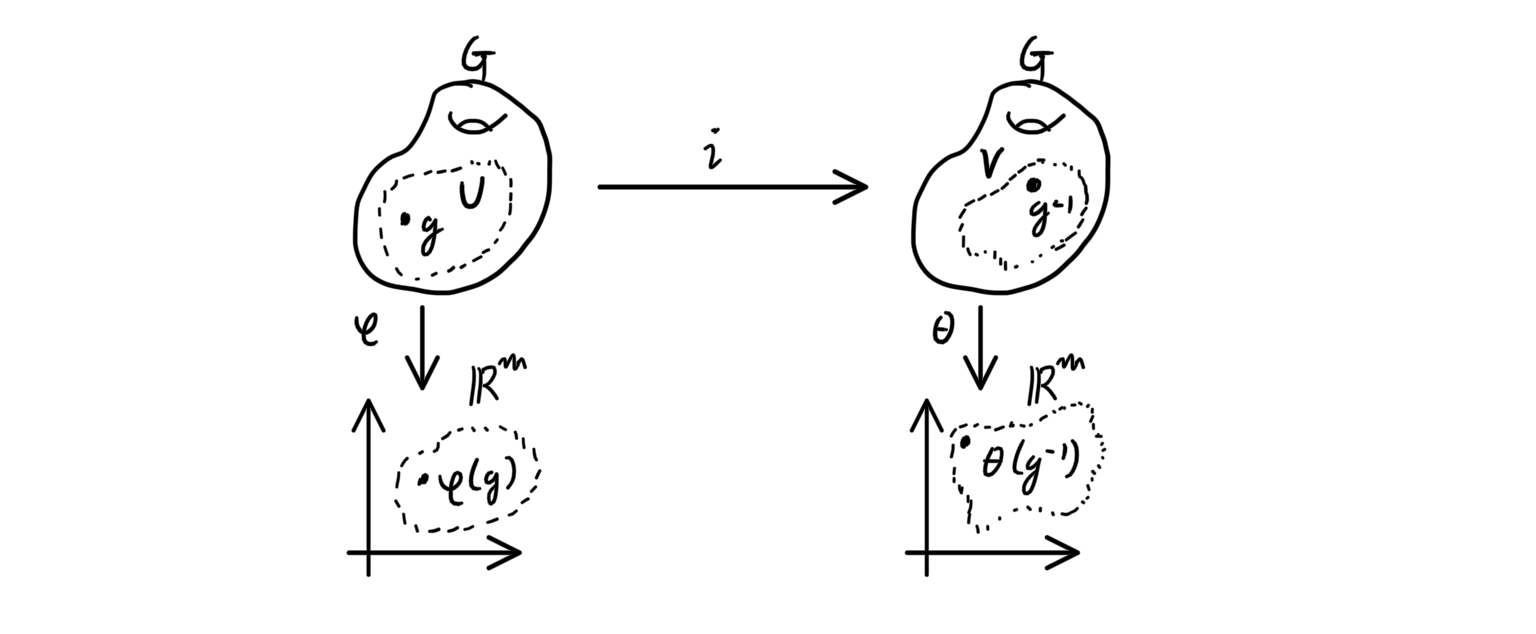
\includegraphics[scale=0.27]{img/Lie_Group_Inversion.PNG}
      \end{center}

    \end{enumerate}
    \end{definition}

    \begin{definition}[Lie Group Homomorphism]
      \label{def:lie-group-homomorphism}
    If $G$ and $H$ are \hyperref[def:lie-group]{Lie groups}, a \textit{Lie group homomorphism} from $G$ to $H$ is a smooth map $F: G \longrightarrow H$ that is also a \hyperref[alg-def:group-homomorphism]{group homomorphism}. 
    The smoothness of $F$ (a smooth property) and its preservance of the \hyperref[alg-def:algebraic-structure]{algebraic structure} of $G$ (an algebraic property) can be comphrensively shown in the commutative diagram below.
    \begin{equation}
      \begin{tikzcd}
        \mathbb{R}^m \times \mathbb{R}^m & G \times G \arrow{l}{\varphi \times \varphi} \arrow{r}{m_1} \arrow{d}{F \times F} & G \arrow{r}{\varphi} \arrow{d}{F} & \mathbb{R}^m \\
        \mathbb{R}^n \times \mathbb{R}^n & H \times H \arrow{l}{\psi \times \psi} \arrow{r}{m_2} & H \arrow{r}{\psi} & \mathbb{R}^n
      \end{tikzcd}
    \end{equation}
    Note that
    \begin{enumerate}
      \item $\varphi \times m_1 \times (\varphi \times \varphi)^{-1} : \mathbb{R}^m \times \mathbb{R}^m \longrightarrow \mathbb{R}^m$ and $\psi \circ m_2 \circ (\psi \times \psi)^{-1}: \mathbb{R}^n \times \mathbb{R}^n \longrightarrow \mathbb{R}^n$ are smooth since $G$ and $H$ are Lie groups. 

      \item $F \circ m_1: G \times G \longrightarrow H$ and $m_2 \circ (F \times F): G \times G \longrightarrow H$ are smooth since $F$ is a Lie group homomorphism. Note that since $F \circ m_1$ and $m_2 \circ (F \times F)$ are \hyperref[def:smooth-maps-between-manifolds]{smooth maps between manifolds}, it really means that the maps 

      \begin{align*}
        \psi \circ F \circ m_1 \circ (\varphi \times \varphi)^{-1}: &\mathbb{R}^m \times \mathbb{R}^m \longrightarrow \mathbb{R}^n \\
        \psi \circ m_2 \circ (F \times F) \circ (\varphi \times \varphi)^{-1}: &\mathbb{R}^m \times \mathbb{R}^m \longrightarrow \mathbb{R}^n
      \end{align*}

      are smooth in the Euclidean sense. 
    \end{enumerate}

    $F$ is called a \textit{Lie group isomorphism} if it is also a \hyperref[def:diffeomorphism-2]{diffeomorphism}, which implies that it has an inverse that is also a Lie group homomorphism. This means that $G$ and $H$ are \textit{isomorphic Lie groups}, meaning that they are indistinguishable as topological spaces, smooth manifolds, and as algebraic structures. 
    \end{definition}

  \subsection{Smooth Covering Maps, Proper Maps}

    TBD
    TBD

  \subsection{Partitions of Unity}

    Recall the Gluing Lemma from topology, which allows us to construct continuous maps by "gluing together" maps defined on subspaces. 

    \begin{lemma}[Pasting Lemma, Gluing Lemma]
      \label{thm:pasting-lemma-gluing-lemma}
      Let $X = A \cup B$, where $A, B$ are closed in $X$. Let $f: A \longrightarrow Y$ and $g: B \longrightarrow Y$ be continuous. If 

        \begin{equation}
          f(x) = g(x) \text{ for all } x \in A \cap B
        \end{equation}

      Then $f$ and $g$ can be combined to form a \hyperref[pst-def:continuous_func]{continuous function} $h: X \longrightarrow Y$, defined

        \begin{equation}
          h(x) \equiv \begin{cases}
                      f(x) & x \in A \setminus B \\
                      f(x) \text{ or } g(x) & x \in A \cap B \\
                      g(x) & x \in B \setminus A
                  \end{cases}
        \end{equation}
    \end{lemma}

    For smooth manifolds, however, the gluing lemma is of limited usefulness, since the produced map, while continuous, is rarely smooth. Observe the following example. 

    \begin{example}[Gluing One-Sided Functions]
      \label{ex:gluing-one-sided-functions}
      Given two functions $f_+: [0, \infty) \longrightarrow \mathbb{R}$ and $f_-: (-\infty, 0] \longrightarrow \mathbb{R}$ defined by 
      \begin{align*}
        f_+(x) = + x, & x \in [0, \infty) \\
        f_-(x) = - x, & x \in (-\infty, 0]
      \end{align*}
      are both smooth and agree at the point $0$ where they overlap, but the continuous map $f: \mathbb{R} \longrightarrow \mathbb{R}$ that they define, $f(x) = |x|$, is not smooth at the origin. 
    \end{example}

    Partitions of unity solves this problem as tools for patching together local smooth maps into global ones. We must first establish the existence of smooth functions that are positive in a specified part of a manifold and identically zero in some other part. 

    \begin{lemma}[Smoothness of $e^{-1/t}$]
      \label{thm:smoothness-of-e1t}
      The function $f: \mathbb{R} \longrightarrow \mathbb{R}$ defined by 
      \begin{equation}
        f(t) \equiv \begin{cases}
                    e^{-1/t} & t > 0 \\
                    0 & t \leq 0
              \end{cases}
      \end{equation}
      is smooth. 
    \end{lemma}
    \begin{proof}
      By induction, showing that the $k$th derivative of $f$ is of the form
        \begin{equation}
          f^{(k)} (t) = \frac{p_k (t)}{t^{2k}} e^{-1/t}
        \end{equation}
    \end{proof}

    \begin{lemma}[Cutoff Function]
      \label{thm:cutoff-function}
      There exists a smooth function $h: \mathbb{R} \longrightarrow \mathbb{R}$, called the \textit{cutoff function}, such that 
      \begin{equation}
        h(t) \equiv \begin{cases}
                    1 & t \leq 1 \\
                    0 < h(t) < 1 & 1 < t < 2 \\
                    0 & t \geq 2
              \end{cases}
      \end{equation}
    \end{lemma}

    \begin{definition}[Support of $f$]
      \label{def:support-of-f}
      If $f$ is any real-valued or vector-valued function on a topological space $M$, the \textit{support of $f$}, denoted by supp$f$, is the closure of the set of points where $f$ is nonzero. 

        \begin{equation}
          \text{supp} f \equiv \text{cl} \big(\{p \in M\;|\; f(p) \neq 0\}\big)
        \end{equation}

      If supp$f$ is contained in some set $U$, we say that $f$ is \textit{supported in $U$}. A function $f$ is said to be \textit{compactly supported} if supp$f$ is a compact set. Clearly, every function on a \hyperref[pst-def:compact-space]{compact space} is compactly supported. 
    \end{definition}

    \begin{lemma}[Smooth Bump Function on $\mathbb{R}^n$]
      \label{thm:smooth-bump-function-on-rn}
      There is a smooth function $H: \mathbb{R}^n \longrightarrow \mathbb{R}$ such that $0 \leq H(x) \leq 1$ everywhere, $H \equiv 1$ on $\bar{B}_1 (0)$, and supp$H = \bar{B}_2 (0)$, where $B_i (c)$ is the open ball with radius $i$ centered at $c$. 
    \end{lemma}
    \begin{proof}
      Just set $H(x) = h(\|x\|)$,  where $h$ is the \hyperref[thm:cutoff-function]{cutoff function}. 
    \end{proof}

    We can visualize the function $H$ in the preceding lemma by assigning a greyscale color to the space $\mathbb{R}^n$ ($1$ representing black, $0$ representing white, and everything in between is greyscale). Then, $H$ would produce a black closed ball of radius $1$ in $\mathbb{R}^n$, with a smoothly changing shade of grey outside the ball of radius $1$ but in the ball of radius $2$, which then smoothly transitions to white for the rest of $\mathbb{R}^n \setminus B_2 (0)$. 

    The function $H$ constructed in this lemma is an example of a \textit{smooth bump function}, a smooth real-valued function that is equal to $1$ on a specified \hyperref[pst-def:closed]{closed set} (in this case, $\bar{B}_1 (0)$) and is supported in a specified \hyperref[pst-def:open-set]{open set} (in this case, any open set containing $\bar{B}_2 (0)$). Later, we will generalize this notion to manifolds. 

    \subsubsection{Paracompactness}

      In order to rigorously define the existence of partitions of unity, we must introduce some technical definitions. The biggest takeaway from this section is that a smooth manifold $M$ that is paracompact admits a smooth partition of unity. 

      \begin{definition}[Locally Finite]
        \label{def:locally-finite}
        Let $X$ be a topological space. A collection $\mathcal{U}$ of subsets of $X$ is said to be \textit{locally finite} if each point of $X$ has a neighborhood that intersects at most finite many of the sets in $\mathcal{U}$. 

        Clearly, an open cover of $X$ where each \hyperref[pst-def:open-set]{open set} intersects finitely many others is locally finite.
      \end{definition}

      \begin{definition}[Refinement]
        \label{def:refinement}
        Given an open cover $\mathcal{U}$ of $X$, another open cover $\mathcal{V}$ is called a \textit{refinement} of $\mathcal{U}$ if for each $V \in \mathcal{V}$ there exists some $U \in \mathcal{U}$ such that $V \subset U$ (in a way, $\mathcal{V}$ is finer than $\mathcal{U}$).  
      \end{definition}

      \begin{definition}[Paracompact]
        \label{def:paracompact}
        A topological space $X$ is \textit{paracompact} if every open cover of $X$ admits a \hyperref[def:locally-finite]{locally finite} refinement. 
      \end{definition}

      \begin{theorem}[Smooth Manifolds Are Paracompact]
        \label{thm:smooth-manifolds-are-paracompact}
        Let $M$ be a smooth manifold. Every open cover of $M$ has a regular refinement. In particular, $M$ is paracompact. 
      \end{theorem}

      \begin{definition}[Partition of Unity]
        \label{def:partition-of-unity}
        Let $M$ be a topological space, and let $\mathcal{X} = \{X_\alpha\}_{\alpha \in A}$ be an arbitrary open cover of $M$. A \textit{partition of unity subordinate to $\mathcal{X}$} is a collection of \hyperref[pst-def:continuous_func]{continuous functions} $\{ \psi_\alpha: M \longrightarrow \mathbb{R}\}$ with the following properties. 
        \begin{enumerate}
          \item $0 \leq \psi_\alpha (x) \leq 1$ for all $\alpha \in A$ and all $x \in M$. 
          \item supp$\psi_\alpha \subset X_\alpha$. 
          \item The set of supports $\{$supp$\psi_\alpha\}$ is \hyperref[def:locally-finite]{locally finite}. 
          \item $\sum_{\alpha \in A} \psi_\alpha (x) = 1$ for all $x \in M$. 
        \end{enumerate}
        A \textit{smooth} partition of unity is one for which each of the functions $\psi_\alpha$ is smooth. 
      \end{definition}

      \begin{theorem}[Existence of Partitions of Unity]
        \label{thm:existence-of-partitions-of-unity}
        If $M$ is a smooth manifold and $\mathcal{X} = \{X_\alpha\}_{\alpha \in A}$ is any open cover of $M$, there exists a smooth \hyperref[def:partition-of-unity]{partition of unity} subordinate to $\mathcal{X}$. 
      \end{theorem}

      \begin{theorem}[Existence of Bump Functions]
        \label{thm:existence-of-bump-functions}
        Let $M$ be a smooth manifold. For any \hyperref[pst-def:closed]{closed set} $A \subset M$ and any \hyperref[pst-def:open-set]{open set} $U$ containing $A$, there exists a smooth bump function for $A$ supported in $U$. 
      \end{theorem}

\section{Tangent Vectors}

  In order to utilize linear approximations on smooth manifolds, we introduce the notion of a \hyperref[mv-def:tangent-space]{tangent space} on a manifold. 

  \subsection{Geometric Tangent Vectors}

    Let us assign a \hyperref[lin-def:vector-space]{vector space}, called a \textit{tangent space} to each point in $\mathbb{R}^n$. That is, the \textit{geometric tangent space} to $\mathbb{R}^n$ at the point $a \in \mathbb{R}^n$ is defined

      \begin{equation}
        \mathbb{R}_a^n \equiv \{(a, v) \;|\; v \in \mathbb{R}^n \}
      \end{equation}

    under the natural operations

    \begin{align*}
      v_a + w_a & \equiv (v + w)_a \\
      c (v_a) & \equiv (c v)_a
    \end{align*}

    A \textit{geometric tangent vector} in $\mathbb{R}^n$ is an element of this space, denoted $v_a$, and $\mathbb{R}^n_a \simeq \mathbb{R}^n$. Note that while these tangent spaces are isomorphic, we distinguish them with the subscripts $a$ representing the point. 

    When looking at other sets in Euclidean space, such as $S^{n-1} \subset \mathbb{R}^n$, we can define the tangent space as the space of vectors that are orthogonal to the radial unit vector through $a$. But this definition is limited within the confines of Euclidean space and not for abstract manifolds. Therefore, we must utilize the concept of \hyperref[mv-def:directional-derivative]{directional derivatives}, which is provided by a tangent vector, to construct tangent spaces. 

    For example, a geometric tangent vector $v_a \in \mathbb{R}^n_a$ yields a map

      \begin{equation}
        D_v \big|_a: C^\infty (\mathbb{R}^n) \longrightarrow \mathbb{R}
      \end{equation}

    which takes the directional derivative in the directoin $v$ at $a$.

      \begin{equation}
        D_v \big|_a f = D_v f(a) = \frac{d}{dt} \bigg|_{t=0} f(a + t v)
      \end{equation}

    This differential operation at the point $a$ is linear and satisfies the \hyperref[mv-thm:product-rule-2]{product rule}

      \begin{equation}
        D_v \big|_a (f g) = f(a) D_v \big|_a g +g(a) D_v \big|_a f
      \end{equation}

    If $v_a = v^i e_i |_a$ in terms of the standard basis (where $e_i |_a$ is the basis of $\mathbb{R}^n_a$), then by the \hyperref[mv-thm:chain-rule]{chain rule} $D_v |_a f$ can be written more concretely as

      \begin{equation}
        D_v \big|_a f = v^i \frac{\partial f}{\partial x^i} (a)
      \end{equation}

    \begin{definition}[Derivation at $a$]
      \label{def:derivation-at-a}
      If $a \in \mathbb{R}^n_a$, a \hyperref[lin-def:linear_map]{linear map} $X: C^\infty (\mathbb{R}^n) \longrightarrow \mathbb{R}$ is called a \textit{derivation at $a$} if it satisfies the following \hyperref[mv-thm:product-rule-2]{product rule} 

        \begin{equation}
          X (f g) = f(a) X g + g(a) X f
        \end{equation}

      Furthermore, let $T_a (\mathbb{R}^n)$ denote the set of all derivations of $C^\infty (\mathbb{R}^n)$ at $a$. Let us endow this set with the operations of addition and scalar multiplication 

      \begin{align*}
        (X + Y) f & \equiv X f + Y f \\
        (c X) f & \equiv c (X f)
      \end{align*}

      It can be checked that if $X, Y$ are derivations (i.e. satisfies linearity and the product rule), then $X + Y$ and $c X$ are also derivations, which makes $T_a (\mathbb{R}^n)$ a \hyperref[lin-def:vector-space]{vector space}. 
    \end{definition}

    \begin{theorem}[Tangent Vectors as Directional Derivatives]
      \label{thm:tangent-vectors-as-directional-derivatives}
      For any $a \in \mathbb{R}^n$, the map $v_a \mapsto D_v |_a$ is an isomorphism from $\mathbb{R}_a^n$ to $T_a (\mathbb{R}^n)$. 
    \end{theorem}

    \begin{corollary}[Coordinate Basis of the Tangent Space to $\mathbb{R}^n$]
      \label{thm:coordinate-basis-of-the-tangent-space-to-rn}
      For any $a \in \mathbb{R}^n$, the $n$ derivations 

        \begin{equation}
          \frac{\partial}{\partial x^1} \bigg|_a, ..., \frac{\partial}{\partial x^n} \bigg|_a, \;\; \frac{\partial}{\partial x^i} \bigg|_a f = \frac{\partial f}{\partial x^i} (a)
        \end{equation}

      form a basis for $T_a (\mathbb{R}^n)$, which therefore has dimension $n$. These basis vectors are more commonly known as the \hyperref[mv-def:partial-derivative]{partial derivatives} of the $C^\infty$ function $f$ at the point $a$. 
    \end{corollary}
    \begin{proof}
      Use the fact that 
        \begin{equation}
          \frac{\partial}{\partial x^i} \bigg|_a = D_{e_i} \big|_a
        \end{equation}
    \end{proof}

    So far, given the Euclidean space $\mathbb{R}^n$, we have constructed this: for every $a \in \mathbb{R}^n$, the \hyperref[mv-def:tangent-space]{tangent space} $T_a (\mathbb{R}^n)$ consists of vectors that are also derivations of $C^\infty (\mathbb{R}^n)$. In other words, we can view the tangent space at $a$ as the \hyperref[lin-def:vector-space]{vector space} of linear differential operators that each take in a $C^\infty$ function $f: \mathbb{R}^n \longrightarrow \mathbb{R}$ and outputs the \hyperref[mv-def:directional-derivative]{directional derivative} of $f$ in direction $v$, evaluated at $a$, which is a real number. It turns out that in each tangent space at, say $a \in \mathbb{R}^n$, there exists a basis of directional derivatives (more commonly known as the \hyperref[mv-def:partial-derivative]{partial derivatives}) in direction $e_i$, the basis vectors, and of course, evaluated at point $a$. 

    \subsubsection{Tangent Vectors on Manifolds}

      Before we define tangent spaces on a smooth manifold $M$, recall that the definition of a smooth (or $C^\infty$) function $f: M \longrightarrow \mathbb{R}$ says that there exists a smooth chart $(U, \varphi)$ for $M$ whose domain contains $p$ and the composite function
      \begin{equation}
        f \circ \varphi^{-1}: \mathbb{R}^n \longrightarrow \mathbb{R}
      \end{equation}
      is smooth on the open subset $\varphi(U) \subset \mathbb{R}^n$. In other words, we are defining the smoothness of $f$ really through the smoothness of $f \circ \varphi^{-1}$. 

      \begin{definition}[Derivation at $p$]
        \label{def:derivation-at-p}
        Let $M$ be a smooth manifold and let $p$ be a point of $M$. A \hyperref[lin-def:linear_map]{linear map} $X: C^\infty (M) \longrightarrow \mathbb{R}$ is called a \textit{derivation at $p$} if it satisfies 

          \begin{equation}
            X(f g) = f(p) X g + g(p) X f
          \end{equation}

        for all $f, g \in C^\infty (M)$. The set of all derivatives at $p$ is a \hyperref[lin-def:vector-space]{vector space} called the \textit{\hyperref[mv-def:tangent-space]{tangent space} to $M$ at $p$}, and is denoted by $T_p M$. An element of $T_p M$ is called a \textit{tangent vector at $p$}. 
      \end{definition}

      Therefore, we can think of the \hyperref[mv-def:tangent-space]{tangent space} of point $p$ in a smooth manifold $M$ as the space of all \hyperref[mv-def:directional-derivative]{directional derivatives} of a smooth function 

        \begin{equation}
          f \circ \varphi^{-1}: \mathbb{R}^n \longrightarrow \mathbb{R}
        \end{equation}

      evaluated at the point $\varphi^{-1} (p)$. It is good to visualize tangent vectors to an abstract smooth manifold $M$ as arrows that are tangent to $M$ and whose base points are attached to $M$ at the given point. Theorems about tangent vectors must always be proved using the abstract definition in terms of derivations, but the intuition should be guided by the geometric picture. 

  \subsection{Pushforwards}

    We now observe the way that tangent vectors behave under smooth maps. In the case of a smooth map between Euclidean spaces, the total derivative of the map at a point (represented by its \hyperref[mv-def:jacobian]{Jacobian} matrix) is a \hyperref[lin-def:linear_map]{linear map} that represents the "best linear approximation" to the map near the given point. In the manifold case, there is a similar linear map, but it acts between tangent spaces. 

    \begin{definition}[Pushforward of a Smooth Map]
      \label{def:pushforward-of-a-smooth-map}
      Given smooth manifolds $M$ and $N$ with a smooth map $F: M \longrightarrow N$, we can define for each $p \in M$ a map

        \begin{equation}
          F_*: T_p M \longrightarrow T_{F(p)} M, \; \big(F_* X \big) (f) \equiv X \big( f \circ F \big)
        \end{equation}

      to be the \textit{pushforward associated with $F$}. Note that $X$ is a tangent vector of $M$, while $F_* X$ is a tangent vector of $N$. Furthermore, if $f \in C^\infty(N)$, then $f \circ F \in C^\infty (M)$, which is consistent with the operations. 

      The operation $F_* X$ is clearly linear and it satisfies the \hyperref[mv-thm:product-rule-2]{product rule} because
      \begin{align*}
        (F_* X) (f g) & = X \big((fg) \circ F \big) \\
        & = X \big( (f \circ F) (g \circ F) \big) \\
        & = f \circ F(p) X(g \circ F) + g \circ F(p) X (f \circ F) \\
        & = f\big(F(p)\big) \big( F_* X \big) (g) + g \big( F(p)\big) \big( F_* X\big) (f)
      \end{align*}
    \end{definition}


    \begin{lemma}[Properties of Pushforwards]
      \label{thm:properties-of-pushforwards}
      Let $F: M \longrightarrow N$ and $G: N \longrightarrow P$ be smooth maps, and let $p \in M$. Then, 
      \begin{enumerate}
        \item $F_*: T_p M \longrightarrow T_{F(p)} M$ is linear. 
        \item $(G \circ F)_* = G_* \circ F_* : T_p M \longrightarrow T_{G \circ F (p)} P$. 
        \item $\big( \Id_M \big)_* = \Id_{T_p M} : T_p M \longrightarrow T_p M$. 
        \item If $f$ is a \hyperref[def:diffeomorphism-2]{diffeomorphism}, then $F_*: T_p M \longrightarrow T_{F(p)} N$ is an isomorphism. 
      \end{enumerate}
    \end{lemma}

    Note that while the \hyperref[mv-def:tangent-space]{tangent space} is defined in terms of smooth functions on the whole manifold, coordinate charts are in general defined on open subsets. The key point is that the tangent space is really a purely local construction. 

    \begin{theorem}[Derivations Depend Only on a Neighbourhood]
      \label{thm:derivations-depend-only-on-a-neighbourhood}
      Suppose $M$ is a smooth manifold with $p \in M$ and $X \in T_p M$. If $f$ and $g$ are both smooth functions on $M$ that agree on some neighborhood of $p$, then $X f = X g$. 
    \end{theorem}

    Clearly, this implies that \hyperref[mv-def:tangent-space]{tangent spaces} of open submanifolds can be naturally identified with those of the whole manifold. 

    \begin{theorem}[Tangent Space of an Open Submanifold]
      \label{thm:tangent-space-of-an-open-submanifold}
      Let $M$ be a smooth manifold and let $U \subset M$ be an open submanifold with $i: U \longrightarrow M$ the canonical inclusion map. Then, for any $p \in U$, 

        \begin{equation}
          i_* : T_p U \longrightarrow T_p M
        \end{equation}

      is an isomorphism. 
    \end{theorem}

    This identification of $X$ to $i_* X$ just says that they are the \textit{same derivation}, with the exception that $X$ acts on functions on the bigger manifold $M$ instead of functions on $U$. This is a harmless claim, since functions can be defined locally. This means that any tangent vector $X \in T_p M$ can be unambiguously applied to functions defined only in a neighborhood of $p$ and not necessarily on all of $M$. 

    Note that every finite-dimensional \hyperref[lin-def:vector-space]{vector space} has a natural smooth manifold structure that is independent of any choice of basis or norm. The follow theorem shows that the tangent space to a vector space can be naturally identified with the vector space itself. 

    \begin{theorem}[Tangent Space to a Vector Space]
      \label{thm:tangent-space-to-a-vector-space}
      For each finite dimensional \hyperref[lin-def:vector-space]{vector space} $V$ and each point $a \in V$, there is a \hyperref[cat-def:natural-isomorphism]{natural isomorphism} $V \rightarrow T_a V$ such that for any \hyperref[lin-def:linear_map]{linear map} $L: V \longrightarrow W$ the following diagram commutes. 

      \begin{equation}
        \begin{tikzcd}
                V \arrow{r}{\cong} \arrow{d}{L}& T_aV \arrow{d}{L_*} \\
                W \arrow{r}{\cong} & T_{L_a}W
              \end{tikzcd}
      \end{equation}
    \end{theorem}

  \subsection{Computations in Coordinates}

    The work that we have done is quite abstract, so we will do some down-to-earth computations in local coordinates. Let $(U, \varphi)$ be a smooth coordinate chart on $M$. Note that $\varphi$ is a \hyperref[def:diffeomorphism-2]{diffeomorphism} from $U$ to an open subset $\Tilde{U} \subset \mathbb{R}^n$. Thus, treating $\varphi(U) = \Tilde{U}$ as a submanifold of the manifold $\mathbb{R}^n$, the pushforward of the function $\varphi: U \longrightarrow \mathbb{R}^n$

      \begin{equation}
        \varphi_* : T_p M \longrightarrow T_{\varphi(p)} \mathbb{R}^n
      \end{equation}

    is an isomorphism. We know that $T_{\varphi(p)} \mathbb{R}^n$ has a basis consisting of the derivations $\partial /\partial x^i \big|_{\varphi(p)}, i = 1, 2, ..., n$. Therefore, the pushforwards of these vectors under $(\varphi^{-1})_*$ form a basis for $T_p M$. The images of these vectors will be denoted

      \begin{equation}
        \frac{\partial}{\partial x^i} \bigg|_p = \big( \varphi^{-1} \big)_* \frac{\partial}{\partial x^i} \bigg|_{\varphi(p)}
      \end{equation}

    It is clear that $\partial / \partial x^i \big|_p $ acts on smooth functions $f: U \longrightarrow \mathbb{R}$ by

      \begin{equation}
        \frac{\partial}{\partial x^i} \bigg|_p \equiv \frac{\partial}{\partial x^i} \bigg|_{\varphi(p)} \big( f \circ \varphi^{-1} \big) = \frac{\partial \hat{f}}{\partial x^i} (\hat{p})
      \end{equation}

    where $\hat{f} = f \circ \varphi^{-1}$ is the coordinate representation of $f$, and $\hat{p} = (p^1, ..., p^n) = \varphi(p)$ is the coordinate representation of $p$. This can be summarized in the following lemma. 

    \begin{lemma}[Dimension and Coordinate Basis of $T_p M$]
      \label{thm:dimension-and-coordinate-basis-of-tpm}
      Let $M$ be a smooth manifold. For any $p \in M$, $T_p M$ is an $n$-dimensional \hyperref[lin-def:vector-space]{vector space}. If $\big( U, (x^i)\big)$ is any smooth chart containing $p$, the coordinate vectors 

        \begin{equation}
          \bigg\{ \frac{\partial}{\partial x^1} \bigg|_p, ..., \frac{\partial}{\partial x^n} \bigg|_p \bigg\}
        \end{equation}

      form a basis for $T_p M$. Thus any tangent vector can be written uniquely as a \hyperref[lin-def:linear-combination]{linear combination}. 

        \begin{equation}
          X = X^i \frac{\partial}{\partial x^i} \bigg|_p
        \end{equation}

      using the summation convention. 
    \end{lemma}

    The numbers $X^i$ are the \textit{components} of $X$. If $X$ is known, its components can be computed easily from its action on the coordinate functions. That is, for each $j$, we can think of $x^j$ (which outputs the $j$th component of a vector) as a smooth real valued function on $U$, to get

      \begin{equation}
        X \big(x^j\big) = \bigg(X^i \frac{\partial}{\partial x^i} \bigg|_p \bigg) \big(x^j \big) = X^i \frac{\partial x^j}{\partial x^i} (p) = X^j
      \end{equation}

    Abridged, the components of $X$ are given by $X^j = X(x^j)$. 

    Now, we observe how pushforwards look in coordinates, starting off with maps between Euclidean spaces. Let $F: U \subset \mathbb{R}^n \longrightarrow V \subset \mathbb{R}^n$ be a smooth map ($U, V$ \hyperref[pst-def:open-set]{open sets} in their respective spaces). For any $p \in U$, the pushforward is a \hyperref[lin-def:linear_map]{linear map} $F_* : T_p \mathbb{R}^n \longrightarrow T_{F(p)} \mathbb{R}^m$, which has a certain matrix representation under the standard basis coordinates. Taking a typical basis vector $\partial/\partial x^i \big|_p$ in $T_p \mathbb{R}^n$, we find its image in $T_p \mathbb{R}^m$ under $F_*$. Using the \hyperref[mv-thm:chain-rule]{chain rule}, 

    \begin{align*}
      \bigg( F_* \frac{\partial}{\partial x^i} \bigg|_p \bigg) f & = \frac{\partial}{\partial x^i} \bigg|_p \big( f \circ F \big) = \frac{\partial f}{\partial y^j} \big( F(p)\big) \frac{\partial F^j}{\partial x^i} (p) \\
      & = \bigg( \frac{\partial F^j}{\partial x^i} (p) \frac{\partial}{\partial y^j} \bigg|_{F(p)} \bigg) f 
    \end{align*}

    Thus, 

      \begin{equation}
        F_* \frac{\partial}{\partial x^i} \bigg|_p = \frac{\partial F^j}{\partial x^i} (p) \frac{\partial}{\partial y^j} \bigg|_{F(p)}
      \end{equation}

    This means that the matrix of the pushforward $F_*$ in terms of standard coordinate bases is precisely the \hyperref[mv-def:jacobian]{Jacobian} matrix, or total derivative, of $F$. 
    
      \begin{equation}
        \begin{pmatrix}
              \frac{\partial F^1}{\partial x^1} (p) & ... & \frac{\partial F^1}{\partial x^n} (p) \\
              ... & ... & ... \\
              \frac{\partial F^m}{\partial x^1} (p) & ... & \frac{\partial F^m}{\partial x^n} (p)
              \end{pmatrix}
      \end{equation}

    Therefore, $F_*: T_p \mathbb{R}^n \longrightarrow T_p \mathbb{R}^m$ corresponds to the total derivative $D F (p): \mathbb{R}^n \longrightarrow \mathbb{R}^m$. Now considering the more general case of smooth maps between smooth manifolds: $F: M \longrightarrow N$, the derivation is not very different. Choosing smooth coordinate charts $(U, \varphi)$ for $M$ near $p$ and $(V, \psi)$ for $N$ near $F(p)$, we obtain the coordinate representation 

      \begin{equation}
        \hat{F} \equiv \psi \circ F \circ \varphi^{-1}: \varphi \big( U \cap F^{-1} (V) \big) \longrightarrow \psi (V)
      \end{equation}

    Using the fact that $F \circ \varphi^{-1} = \psi^{-1} \circ \hat{F}$, we compute $F_*: T_p M \longrightarrow T_p N$

    \begin{align*}
      F_* \frac{\partial}{\partial x^i} \bigg|_p & = F_* \bigg( ( \varphi^{-1} )_* \frac{\partial}{\partial x^i} \bigg|_{\varphi(p)} \bigg) \\
      & = (\psi^{-1})_* \bigg( \hat{F}_* \frac{\partial}{\partial x^i} \bigg|_{\varphi(p)}\bigg) \\ 
      & = (\psi^{-1})_* \bigg( \frac{\partial \hat{F}^j}{\partial x^i} (\hat{p}) \frac{\partial}{\partial y^j} \bigg|_{\hat{F}(\varphi(p))} \bigg) \\
      & = \frac{\partial \hat{F}^j}{\partial x^i} (\hat{p})\, \frac{\partial}{\partial y^j} \bigg|_{F(p)} 
    \end{align*}

    Thus, $F_*: T_p M \longrightarrow T_p N$ is represented in terms of the coordinate bases by the Jacobian matrix of the coordinate representation of $F$. One can see that the concept of the pushforward allows us to abstractify the Jacobian matrix into an abstract linear transformation from $T_p M$ to $T_p N$. Because of this, the \hyperref[def:pushforward-of-a-smooth-map]{pushforward of a smooth map} $F: M \longrightarrow N$ is sometimes called its differential or its total derivative. We will denote $F_*$ for the pushforward of a smooth map between smooth manifolds and $DF(p)$ for the total derivative of a map between finite dimensional \hyperref[lin-def:vector-space]{vector spaces}. 

    \subsubsection{Change of Coordinates}

      Let $(U, \varphi)$ and $(V, \psi)$ be two smooth charts on $M$ with $p \in U \cap V$. Let us denote the coordinate function of $\varphi$ by $(x^i)$ and those of $\psi$ by $( \Tilde{x}^i)$. Then, any tangent vector at $p$ can be represented to either basis $ \big( \partial/\partial x^i \big|_p \big)$ or $\big( \partial/\partial \Tilde{x}^i \big|_p \big)$. 

      It isn't too difficult to find out how these two representations are related. With the transition map 

        \begin{equation}
          \psi \circ \varphi^{-1} : \varphi(U \cap V) \longrightarrow \psi (U \cap V), \;\; \psi \circ \varphi^{-1} (x) = \big( \Tilde{x}^1 (x), ..., \Tilde{x}^n (x) \big)
        \end{equation}

      the pushforward of $\psi \circ \varphi^{-1} \in$ End$(T_p \mathbb{R}^n)$ can be written

        \begin{equation}
          \big( \psi \circ \varphi^{-1}\big)_* \frac{\partial}{\partial x^i} \bigg|_{\varphi(p)} = \frac{\partial \Tilde{x}^j}{\partial x^i} \big( \varphi(p) \big) \frac{\partial}{\partial \Tilde{x}^j} \bigg|_{\psi(p)}
        \end{equation}

      Letting $\bar{p} = \varphi(p)$, we compute

      \begin{align*}
        \frac{\partial}{\partial x^i} \bigg|_p & = \big( \varphi^{-1} \big)_* \frac{\partial}{\partial x_i} \bigg|_{\varphi(p)} = \big( \varphi^{-1} \big)_* \big( \psi \circ \varphi^{-1} \big)_* \frac{\partial}{\partial x_i} \bigg|_{\varphi(p)} \\ 
        & = \big( \psi^{-1}\big)_* \frac{\partial \Tilde{x}^j}{\partial x^i} \big( \varphi(p)\big) \frac{\partial}{\partial \Tilde{x}^j} \bigg|_{\psi(p)} = \frac{\partial \Tilde{x}^j}{\partial x^i} \big( \varphi(p)\big) \big( \psi^{-1}\big)_* \frac{\partial}{\partial \Tilde{x}^j} \bigg|_{\psi (p)} \\
        & = \frac{\partial \Tilde{x}^j}{\partial x^i} (\hat{p}) \frac{\partial}{\partial \Tilde{x}^j} \bigg|_p
      \end{align*}

      This formula conveniently, looks exactly like the multivariate chain rule of \hyperref[mv-def:partial-derivative]{partial derivatives} in $\mathbb{R}^n$. Applying this to the components of a vector, 

      \begin{align*}
        X = X^i \frac{\partial}{\partial x^i} \bigg|_p & = X^i \bigg( \frac{\partial \Tilde{x}^j}{\partial x^i} (\hat{p}) \frac{\partial}{\partial \Tilde{x}^j} \bigg|_p \bigg) \\
        & = \bigg(X^i \frac{\partial \Tilde{x}^j}{\partial x^i} (\hat{p}) \bigg) \frac{\partial}{\partial \Tilde{x}^j} \bigg|_p =
        \Tilde{X}^j \frac{\partial}{\partial \Tilde{x}^j} \bigg|_p
      \end{align*}

      We can find that the components transform by the rule 

        \begin{equation}
          \Tilde{X}^j = \frac{\partial \Tilde{x}^j}{\partial x^i} (\hat{p}) X^i
        \end{equation}

  \subsection{Tangent Vectors to Curves}

    \begin{definition}[Curve]
      \label{def:curve}
      We define a \textit{curve} in manifold $M$ to be a continuous map 

        \begin{equation}
          \gamma: J \longrightarrow M
        \end{equation}

      where $J \subset \mathbb{R}$ is an interval. 
    \end{definition}

    Our construction of tangent vectors and pushforwards leads to a very natural definition of tangent vectors of curves in manifolds. 

    \begin{definition}[Tangent Vector to a Curve]
      \label{def:tangent-vector-to-a-curve}
      If $\gamma$ is a smooth curve in smooth manifold $M$, the \textit{tangent vector} to $\gamma$ at $t_0 \in J$ is the vector 

        \begin{equation}
          \gamma^\prime (t_0) \equiv \gamma_* \bigg( \frac{d}{dt} \bigg|_{t_0} \bigg) \in T_{\gamma(t_0)} M
        \end{equation}

      where $d/dt \big|_{t_0}$ is the standard coordinate basis vector for the 1 dimensional $T_{t_0} \mathbb{R}$. 
    \end{definition}

    The tangent vector acts on $C^\infty(M)$ functions $f$ (that is, $f: M \longrightarrow \mathbb{R}$) by

      \begin{equation}
        \gamma^\prime (t_0) f = \bigg( \gamma_* \frac{d}{dt} \bigg|_{t_0} \bigg) f = \frac{d}{dt} \bigg|_{t_0} (f \circ \gamma) = \frac{d (f \circ \gamma)}{dt} (t_0)
      \end{equation}
    
    where $f \circ \gamma: \mathbb{R} \longrightarrow \mathbb{R}$. In other words, $\gamma^\prime (t_0)$ is the derivation at $\gamma(t_0)$ obtained by taking the derivative of a function along $\gamma$. Note also that the path function $\gamma$ is also a smooth map between manifolds. 

    Let $(U, \varphi)$ be a smooth chart with coordinate functions $(x^i)$. If $\gamma(t_0) \in U$, we can write the coordinate representation of $\gamma$ as $\gamma(t) = \big( \gamma^1 (t), ..., \gamma^n (t)\big)$ for $t$ near $t_0$. (Note that explicitly speaking, we are really writing the shorthand form of $(\varphi \circ \gamma) (t) = \big( (\varphi \circ \gamma)^1 (t), ..., (\varphi \circ \gamma)^n (t)\big)$). Then, the formula  for the pushforward in coordinates becomes 

      \begin{equation}
        \gamma^\prime (t_0) = (\gamma^i)^\prime (t_0) \frac{\partial}{\partial x^i} \bigg|_{\gamma(t_0)}
      \end{equation}

    This means that $\gamma^\prime (t_0)$ is given by essentially the same formula sit would be in Euclidean space: It is the tangent vector whose components in a coordinate basis are the derivatives of the component functions of $\gamma$. 

    \begin{lemma}[Every Tangent Vector Is Tangent to a Curve]
      \label{thm:every-tangent-vector-is-tangent-to-a-curve}
      Let $M$ be a smooth manifold and $p \in M$. Then, every $X \in T_p M$ is the tangent vector to some smooth curve in $M$. 
    \end{lemma}

    This lemma tells us that we can think of the \hyperref[mv-def:tangent-space]{tangent space} at $p$ as the set of tangent vectors to smooth curves in $M$ passing through $p$. Similar results hold under compositions of smooth maps. 

    \begin{theorem}[Pushforward of a Velocity Vector]
      \label{thm:pushforward-of-a-velocity-vector}
      Let $F: M \longrightarrow N$ be a smooth map, and let $\gamma: J \longrightarrow M$ be a smooth curve. For any $t_0 \in J$, the tangent vector at $t = t_0$ to the composite curve $F \circ \gamma: J \longrightarrow N$ is given by 

        \begin{equation}
          (F \circ \gamma)^\prime (t_0) = F_* \big( \gamma^\prime (t_0) \big)
        \end{equation}

      We can think of this composition as the double pushforward of the basis vector $d/dt \big|_{t_0}$ to $T_{\gamma(t_0)} M$ first and $T_{(F \circ \gamma)(t_0)} N$ second). 
    \end{theorem}

\section{Vector Fields}

  \subsection{The Tangent Bundle}

    \begin{definition}[Tangent Bundle of $M$]
      \label{def:tangent-bundle-of-m}
      For any smooth manifold $M$, we define the \textit{tangent bundle of $M$}, denoted $TM$ to be the disjoint union of the \hyperref[mv-def:tangent-space]{tangent spaces} at all points of $M$. 

        \begin{equation}
          TM \equiv \bigsqcup_{p \in M} T_p M
        \end{equation}

      Elements of $TM$ are written as an ordered pair 

        \begin{equation}
          \big(p, X \big) \text{ or } X_p, \;\; p \in M, X \in T_p M
        \end{equation}

      The tangent bundle also comes with an natural \textit{projection map}

        \begin{equation}
          \pi: TM \longrightarrow M, \;\; \pi \big(p, X\big) = p
        \end{equation}

      which sends each vector in $T_p M$ to the point $p$ at which it is tangent. 
    \end{definition}

    The following lemma reveals an important property of tangent bundles. 

    \begin{lemma}[Smooth Structure on the Tangent Bundle]
      \label{thm:smooth-structure-on-the-tangent-bundle}
      For any smooth $n$-manifold $M$, the tangent bundle $TM$ has a natural topology and smooth structure that make it into a $2n$-dimensional smooth manifold. With this structure, 
        \begin{equation}
          \pi: TM \longrightarrow M
        \end{equation}
      is a smooth map. 
    \end{lemma}

  \subsection{Vector Fields on Manifolds}

    \begin{definition}[Vector Field on $M$]
      \label{def:vector-field-on-m}
      Given a smooth manifold $M$, a \textit{vector field on $M$} is a continuous map 

        \begin{equation}
          Y: M \longrightarrow TM, \;\; p \mapsto Y_p
        \end{equation}

      with the property that 

        \begin{equation}
          \pi \circ Y = \Id_M
        \end{equation}

      or equivalently, $Y_p \in T_p M$ for each $p \in M$. We also say that the vector field is a \textit{section} (as in \textit{cross section}) of the map $\pi: TM \longrightarrow M$ (i.e. a continuous right inverse of $\pi$). 
    \end{definition}

    While each vector in the vector field $Y$ "lives" in distinct \hyperref[mv-def:tangent-space]{tangent spaces}, we can visualize a vector field on manifold $M$ as an arrow attached to each point of $M$, chosen to be tangent to $M$ and to vary continuously from point to point. 

    \begin{definition}[Smooth and Rough Vector Fields]
      \label{def:smooth-and-rough-vector-fields}
      A \textit{smooth vector field} is a smooth map from $M$ to $TM$. A \textit{rough vector field} is a (not necessarily continuous) map $Y: M \longrightarrow TM$ satisfying the condition that $\pi\circ Y = \Id_M$. 
    \end{definition}

    If $Y: M \longrightarrow TM$ is a rough vector field and $\big( U, (x^i)\big)$ is any smooth coordinate chart for $M$, we can write the value of $Y$ at any point $p \in U$ in terms of the coordinate basis vectors. 

      \begin{equation}
        Y_p = Y^i (p) \frac{\partial}{\partial x^i} \bigg|_p
      \end{equation}

    This defines $n$ functions $Y^i: U \longrightarrow \mathbb{R}$, called the \textit{component functions} of $Y$ in the given chart. 

    \begin{lemma}[Smoothness Criterion for Vector Fields]
      \label{thm:smoothness-criterion-for-vector-fields}
      Let $M$ be a smooth manifold, and let $Y: M \longrightarrow TM$ be a rough vector field. If $\big( U, (x^i)\big)$ is any smooth coordinate chart on $M$, then $Y$ is smooth on $U$ if and only if its component functions with respect to this chart are smooth. 
    \end{lemma}

    With this lemma, it is now sufficient to check the smoothness of the component functions in order to check the smoothness of the entire vector field. The next lemma shows that every tangent vector at a point can be extended to a smooth global vector field. 

    \begin{lemma}[Extending a Tangent Vector to a Global Vector Field]
      \label{thm:extending-a-tangent-vector-to-a-global-vector}
      Let $M$ be a smooth manifold. If $p \in M$ and $X \in T_p M$, then there exists a smooth vector field $\Tilde{X}$ on $M$ such that $\Tilde{X}_p = X$. 
    \end{lemma}

    \begin{definition}[Support of a Vector Field]
      \label{def:support-of-a-vector-field}
      Just as for functions, the \textit{support} of a vector field $Y$ is defined to be the closure of the set $\{ p \in M\;|\; Y_p \neq 0\}$. A vector field is said to be compactly supported if its support is a compact set. 
    \end{definition}

    Furthermore, if $U$ is any \hyperref[pst-def:open-set]{open set} of $M$, the fact that $T_p U$ is naturally identified with $T_p M$ for each $p \in U$ allows us to identify the subset $\pi^{-1} (U) \subset TM$. Therefore, a vector field on $U$ can be thought of either as a map from $U$ to $TU$ or a map from $U$ to $TM$. If $Y$ is a vector field on $M$, its restriction $Y |_U$ is a vector field on $U$, which is smooth if $Y$ is. 

    \begin{definition}[The Space of Smooth Vector Fields]
      \label{def:the-space-of-smooth-vector-fields}
      Let us denote the set of all smooth vector fields on $M$ as $\mathcal{T}(M)$. It is a \hyperref[lin-def:vector-space]{vector space} under pointwise addition and scalar multiplication. That is, given $Y, Z \in \mathcal{T}(M)$

        \begin{equation}
          (a Y + b Z)_p = a Y_p + b Z_p
        \end{equation}

      The zero element of this vector space is also the zero vector field. In addition, smooth vector fields can be multiplied by smooth real-valued functions. That is, if $f \in C^\infty (M)$ and $Y \in \mathcal{T}(M)$, then we can define $f Y: M \longrightarrow TM$ as 

        \begin{equation}
          (fY)_p = f(p) Y_p
        \end{equation}
    \end{definition}

    The coordinate representation of a vector field $Y$ can also be written as an equation between vector fields rather than at a single point.

      \begin{equation}
        Y_p = Y^i (p) \frac{\partial}{\partial x^i} \bigg|_p \implies Y = Y^i \frac{\partial}{\partial x^i}
      \end{equation}

    A property of vector fields is that they induce operators on the space of smooth real-valued functions $C^\infty (M)$. That is, if $Y \in \mathcal{T}(M)$ and $f \in C^\infty (U)$, where $U$ is an \hyperref[pst-def:open-set]{open set} in $M$, then we obtain a new function $Y f: U \longrightarrow \mathbb{R}$, defined 

      \begin{equation}
        Y f \equiv Y^i \frac{\partial}{\partial x^i} (f) \implies Y f(p) \equiv Y_p f \equiv Y^i (p) \frac{\partial}{\partial x^i} f \bigg|_p
      \end{equation}

    Note that there is a concrete difference between $Y f$ and $f Y$. $Y f$ is a real valued function shown above, while $f Y$ is a smooth vector field gotten by multiplying the vector produced by $Y$ at point $p$ ($Y_p$) with the value of $f$ at $p$ ($f(p)$). Because the action of a tangent vector on a function is determined by the values of the function in an arbitrarily small neighborhood, it follows that $Y f$ is locally determined. This leads to another sufficient condition for smoothness of vector fields. 

    \begin{lemma}[Smoothness Criterion for a Rough Vector Field]
      \label{thm:smoothness-criterion-for-a-rough-vector-field}
      Let $M$ be a smooth manifold, and let $Y: M \longrightarrow TM$ be a rough vector field. Then, $Y$ is smooth if and only if for every \hyperref[pst-def:open-set]{open set} $U \subset M$ and every $f \in C^\infty (U)$, the function $Y f: U \longrightarrow \mathbb{R}$ is smooth. 
    \end{lemma}

    Notice that due to to this lemma, a smooth vector field $Y \in \mathcal{T}(M)$ defines a map from $C^\infty(M)$ to itself by the mapping $f \mapsto Y f$. This is clearly linear over $\mathbb{R}$ and satisfies the \hyperref[mv-thm:product-rule-2]{product rule} 
      \begin{equation}
        Y(f g) = f Y g + g Y f
      \end{equation}
    since it satisfies for arbitrary point $p \in M$. 

    \begin{definition}[Derivation of $C^\infty(M)$]
      \label{def:derivation-of-cinftym}
      A linear endomorphism $Y$ of $C^\infty (M)$ satisfying 

        \begin{equation}
          Y(f g) = f Y g + g Y f, \; f, g \in C^\infty(M)
        \end{equation}

      is called a \textit{derivation} of $C^\infty (M)$. 
    \end{definition}

    The next theorem shows that derivations of $C^\infty (M)$ can be identified with smooth vector fields. 

    \begin{theorem}[Vector Fields as Derivations of $C^\infty(M)$]
      \label{thm:vector-fields-as-derivations-of-cinftym}
      Let $M$ be a smooth manifold. A map $\mathcal{Y}: C^\infty (M) \longrightarrow C^\infty (M)$ is a derivation if and only if it is of the form $\mathcal{Y} f = Y f$ for some smooth vector field $Y \in \mathcal{T}(M)$. 
    \end{theorem}

    \subsubsection{Pushforwards of Vector Fields}

      If $F: M \longrightarrow N$ is a smooth map and $Y$ is a vector field on $M$, then for each point $p \in M$, we obtain a vector $F_* Y_p \in T_{F(p)} N$ by pushing forward $Y_p$. However, this does not in general define a vector field on $N$. For example, if $F$ is not surjective, we cannot assign a vector to point $q \in N \setminus F(M)$. If $F$ is not injective, then for some point of $N$ there may be several different vectors obtained as pushforwards of $Y$ from different points of $M$. Therefore, vector fields do not always push forward. 

      \begin{definition}[$F$-Related Vector Fields]
        \label{def:f-related-vector-fields}
        If $F: M \longrightarrow N$ is smooth and $Y$ is a vector field on $M$, suppose there happens to be a vector $Z$ on $N$ with the property that for each $p \in M$, $F_* Y_p = Z_{F(p)}$. In this case, we say that the vector fields $Y$ and $Z$ are \textit{$F$-related}. 
      \end{definition}

      The vector field $Z$ in the definition above represents the "closest" vector field on $N$ that we can get that is a pushforward of $Y$. If $F$ is not surjective, the vector field $Z$ can take any value at points $p \in N \setminus F(M)$ (meaning that the $F$-related vector field to $Y$ is not unique). If $F$ is not injective, for all points $a_i$ that map onto $r \in N$, the pushforward of $F$ at each $a_i$ must agree on their output vector in $T_r N$. There is a useful criterion to see if two vector fields are $F$-related. 

      \begin{theorem}[Characterization of $F$-Relatedness]
        \label{thm:characterization-of-f-relatedness}
        Suppose $F: M \longrightarrow N$ is a smooth map, $Y \in \mathcal{T}(M)$, and $Z \in \mathcal{T}(N)$. Then, $Y$ and $Z$ are $F$-related if and only if for every smooth real-valued function defined on an open subset of $N$, 

          \begin{equation}
            Y (f \circ F) = (Z f) \circ F
          \end{equation}
      \end{theorem}

      Note that for a given smooth map $F: M \longrightarrow N$ and vector field $Y \in \mathcal{T}(M)$, there may not be \textit{any} vector field on $N$ that is $F$-related to $Y$. However, there is one special case in which there always exists a unique vector field. 

      \begin{theorem}[Pushforward of a Vector Field by a Diffeomorphism]
        \label{thm:pushforward-of-a-vector-field-by-a}
        Suppose $F: M \longrightarrow N$ is a \hyperref[def:diffeomorphism-2]{diffeomorphism}. For every $Y \in \mathcal{T}(M)$, there is a unique smooth vector field on $N$ that is $F$-related to $Y$. 
      \end{theorem}

      It is quite easy to see why the theorem above is true. Since $F$ is a \hyperref[def:diffeomorphism-2]{diffeomorphism} (and thus a bijectiion), there will be no points on $N$ where the $F$-related vector field $Z$ is undefined (due to surjectivity) and there will be no contradictions in the values of $Z$ (due to injectivity). Finally, $F$ being a diffeomorphism will ensure smoothness of $Z$. . 

      \begin{definition}[Pushforward of $Y$ by $F$]
        \label{def:pushforward-of-y-by-f}
        In the case where $F: M \longrightarrow N$ is a \hyperref[def:diffeomorphism-2]{diffeomorphism}, the unique vector field $F_* Y$ that is $F$-related to $Y$ is called the \textit{pushforward of $Y$ by $F$}. Note that $F_* Y$ is defined only if $F$ is a diffeomorphism.  
      \end{definition}

    \subsubsection{Vector Fields on Manifolds with Boundary}

  \subsection{Lie Brackets}

    We can fix this problem using the Lie bracket operator. 

    \begin{definition}[Lie Bracket]
      \label{def:lie-bracket}
    The operator 

      \begin{equation}
        [\cdot, \cdot]: \mathcal{T}(M) \times \mathcal{T} (M) \longrightarrow \mathcal{T}(M)
      \end{equation}

    is called the \textit{Lie bracket}. Given two vector fields $V, W$ on smooth manifold $M$, we define the $[V, W]$ as 

      \begin{equation}
        [V, W]: C^\infty(M) \longrightarrow C^\infty (M), \;\; [V, W] f \equiv V W f - W V f
      \end{equation}
    \end{definition}

    \begin{lemma}[The Lie Bracket of Smooth Fields Is Smooth]
      \label{thm:the-lie-bracket-of-smooth-fields-is-smooth}
      The \hyperref[def:lie-bracket]{Lie bracket} of any pair of smooth vector fields is a smooth vector field.
    \end{lemma}

    The value of the vector field $[V, W]$ at a point $p \in M$ is the derivation at $p$ given by the formula

      \begin{equation}
        [V, W]_p f \equiv V_p (W f) - W_p (V f)
      \end{equation}

    but the formula is of limited usefulness for practical computations. The following lemma simpliies it greatly. 

    \begin{lemma}[Lie Bracket in Coordinates]
      \label{thm:lie-bracket-in-coordinates}
      Let $V, W$ be smooth vector fields on a smooth manifold $M$, and let

        \begin{equation}
          V = V^i \frac{\partial}{\partial x^i} \text{ and } W = W^j \frac{\partial}{\partial x^j}
        \end{equation}

      be the coordinate expressions for $V$ and $W$ in terms of some smooth local coordinates $(x^i)$ for $M$. Then, $[V, W]$ hsa the following coordinate expression: 

        \begin{equation}
          [V, W] = \bigg( V^i \frac{\partial W^j}{\partial x^i} - W^i \frac{\partial V^j}{\partial x^i}\bigg) \frac{\partial}{\partial x^j}
        \end{equation}

      or more concisely, 
        \begin{equation}
          [V, W] = \big(V W^j - W V^j \big) \frac{\partial}{\partial x^j}
        \end{equation}
    \end{lemma}
    \begin{proof}
      Since $[V, W]$ is a smooth vector field, its values are determined locally. Thus, it suffices to compute in a single smooth chart. 
      \begin{align*}
        [V,W]_f & = V^i \frac{\partial}{\partial x^i} \bigg( W^j \frac{\partial f}{\partial x^j} \bigg) - W^j \frac{\partial}{\partial x^j} \bigg( V^i \frac{\partial f}{\partial x^i} \bigg) \\
        & = V^i \frac{\partial W^j}{\partial x^i} \frac{\partial f}{\partial x^j} + V^i W^j \frac{\partial^2 f}{\partial x^i \partial x^j} - W^j \frac{\partial V^i}{\partial x^j} \frac{\partial f}{\partial x^i} - W^j V^i \frac{\partial^2 f}{\partial x^j \partial x^i} \\
        & = V^i \frac{\partial W^j}{\partial x^i} \frac{\partial f}{\partial x^j} - W^j \frac{\partial V^i}{\partial x^j} \frac{\partial f}{\partial x^i}
      \end{align*}
      where we've used the \hyperref[mv-thm:product-rule-2]{product rule} in the first to second step and the fact that mixed \hyperref[mv-def:partial-derivative]{partial derivatives} of a smooth function are equal in any order. 
    \end{proof}

    \begin{example}[Computing a Lie Bracket on $\mathbb{R}^3$]
      \label{ex:computing-a-lie-bracket-on-r3}
      Let us define smooth vector fields $V, W \in \mathcal{T}(\mathbb{R}^3)$ by 
      \begin{align*}
        V & = x \frac{\partial}{\partial x} + \frac{\partial}{\partial y} + x (y+1) \frac{\partial}{\partial z} \\
        W & = \frac{\partial}{\partial x} + y \frac{\partial}{\partial z}
      \end{align*}
      After some tedious calculations, we compute a total of nine separate terms to get 
      \begin{align*}
        [V, W] & = - \frac{\partial}{\partial x} - (y+1) \frac{\partial}{\partial z} + \frac{\partial}{\partial z} \\
        & = - \frac{\partial}{\partial x} - y \frac{\partial}{\partial z} 
      \end{align*}
    \end{example}

    \begin{lemma}[Properties of the Lie Bracket]
      \label{thm:properties-of-the-lie-bracket}
      The \hyperref[def:lie-bracket]{Lie bracket} satisfies the following identities for all $V, W, X \in \mathcal{T}(M)$. 
      \begin{enumerate}
        \item Bilinearity. For all $a, b \in \mathbb{R}$, 
        \begin{align*}
            [a V + b W, X] & = a [V, X] + b [W, X] \\
            [X, a V + b W] & = a [X, V] + b [X, W]
        \end{align*}

        \item Antisymmetry.
        \begin{equation}
          [V, W] = - [W, V]
        \end{equation}

        \item Jacobi Identity. 
        \begin{equation}
          [V,[W,X]] + [W,[X,V]] + [X,[V,W]] = 0
        \end{equation}

        \item For $f, g \in C^\infty (M)$, 
        \begin{equation}
          [f V, g W] = f g [V, W] + ( fVg) W - (gWf) V
        \end{equation}
      \end{enumerate}
    \end{lemma}

    The next theorem states the naturality of the \hyperref[def:lie-bracket]{Lie bracket}. That is, $F$-relatedness is preserved with the Lie bracket. 

    \begin{theorem}[Lie Brackets Respect $F$-Relatedness]
      \label{thm:lie-brackets-respect-f-relatedness}
      Let $F: M \longrightarrow N$ be a smooth map, and let $V_1, V_2 \in \mathcal{T} (M)$ and $W_1, W_2 \in \mathcal{T}(N)$ be vector fields such that $V_i$ is $F$-related to $W_i$ for $i = 1, 2$. Then, $[V_1, V_2]$ is $F$-related to $[W_1, W_2]$. 
    \end{theorem}

    \begin{corollary}[Diffeomorphisms Preserve Lie Brackets]
      \label{thm:diffeomorphisms-preserve-lie-brackets}
      Suppose $F: M \longrightarrow N$ is a \hyperref[def:diffeomorphism-2]{diffeomorphism} and $V_1, V_2 \in \mathcal{T}(M)$. Then 
        \begin{equation}
          F_* [V_1, V_2] = [F_* V_1, F_* V_2]
        \end{equation}
    \end{corollary}

  \subsection{The Lie Algebra of a Lie Group}

    \begin{definition}[Left and Right Translation]
      \label{def:left-and-right-translation}
      Let $G$ be a \hyperref[def:lie-group]{Lie group}. Any $g \in G$ defines maps $L_g, R_g : G \longrightarrow G$, called \textit{\hyperref[alg-def:left-translation]{left translation}} and \textit{right translation}, respectively, by 
      \begin{align*}
        L_g (h) \equiv g h , & R_g (h) \equiv h g
      \end{align*}
    \end{definition}

    Because $L_g$ can be written as the composition of smooth maps 

      \begin{equation}
        \begin{tikzcd}
              G \arrow{r}{i_g} & G \times G \arrow{r}{m} & G
              \end{tikzcd}
      \end{equation}

    where $i_g (h) \equiv (g, h)$ and $m$ is multiplication, it follows that $L_g$ is smooth. It is actually a \hyperref[def:diffeomorphism-2]{diffeomorphism} of $G$ since $L_{g^{-1}}$ is a smooth inverse for it. The same goes for $R_g$. Notice that given any two points $g_1, g_2 \in G$, there is a unique \hyperref[alg-def:left-translation]{left translation} of $G$ taking $g_1$ to $g_2$. This is the translation $g_2 g_1^{-1}$. Many important \hyperref[def:lie-group]{Lie groups} follow from the fact that we can systematically map any point to any other by such a global diffeomorphism. 

    \begin{definition}[Left-Invariant Vector Field]
      \label{def:left-invariant-vector-field}
      A vector field $X$ on $G$ is said to be \textit{left-invariant} if it is invariant under all \hyperref[alg-def:left-translation]{left translation}, in the sense that it is $L_g$-related to itself for every $g \in G$. More explicitly, this means that
      \begin{align*}
        (L_g)_* X_{g^\prime} = X_{g g^\prime} \text{ for all } g, g^\prime \in G
      \end{align*}
    \end{definition}

    Furthermore, because

      \begin{equation}
        (L_g)_* \big( a X + b Y \big) = a (L_g)_* X + b (L_g)_* Y
      \end{equation}

    the set of all smooth \hyperref[def:left-invariant-vector-field]{left-invariant vector fields} on $G$ is a linear subspace of $\mathcal{T}(M)$. Even further, it is a \textit{\hyperref[alg-def:lie-algebra]{Lie algebra}}, which will be defined shortly.  

    \begin{lemma}[Left-Invariance Is Preserved by the Lie Bracket]
      \label{thm:left-invariance-is-preserved-by-the-lie-bracket}
      Let $G$ be a \hyperref[def:lie-group]{Lie group}, and suppose $X$ and $Y$ are smooth \hyperref[def:left-invariant-vector-field]{left-invariant vector fields} on $G$. Then $[X, Y]$ is left-invariant. 
    \end{lemma}
    \begin{proof}
      Since $(L_g)_* X = X$ and $(L_g)_* Y = Y$ by definition of left-invariance, it follows that

        \begin{equation}
          (L_g)_* [X,Y] = [(L_g)_* X, (L_g)_* Y] = [X,Y]
        \end{equation}

      meaning that $[X, Y]$ is $L_g$-related to itself. 
    \end{proof}

    \begin{definition}[Lie Algebra]
      \label{def:lie-algebra}
      A \textit{Lie algebra} is a real \hyperref[lin-def:vector-space]{vector space} $\mathfrak{g}$ endowed with a map called the \textit{bracket} from $\mathfrak{g} \times \mathfrak{g} \longrightarrow \mathfrak{g}$, usually denoted by $(X, Y) \mapsto [X, Y]$, that satisfies the following properties for all $X, Y, Z \in \mathfrak{g}$. 

      \begin{enumerate}
        \item Bilinearity. For all $a, b \in \mathbb{R}$, 
        \begin{align*}
          [a V + b W, X] & = a [V, X] + b [W, X] \\
          [X, a V + b W] & = a [X, V] + b [X, W]
        \end{align*}

        \item Antisymmetry.
        \begin{equation}
          [V, W] = - [W, V]
        \end{equation}

        \item Jacobi Identity. 
        \begin{equation}
          [V,[W,X]] + [W,[X,V]] + [X,[V,W]] = 0
        \end{equation}
      \end{enumerate}

      Notice that the Jacobi identity is a substitute for associativity, which does not hold in general for brackets in a Lie algebra. 
    \end{definition}

    \begin{definition}[Lie Subalgebra]
      \label{def:lie-subalgebra}
      If $\mathfrak{g}$ is a \hyperref[def:lie-algebra]{Lie algebra}, a linear subspace $\mathfrak{h} \subset \mathfrak{g}$ is called a \textit{Lie subalgebra} of $\mathfrak{g}$ if it is closed under brackets. In other words, $\mathfrak{h}$ is itself a Lie algebra under the restriction of the bracket to $\mathfrak{h}$. 
    \end{definition}

    \begin{definition}[Lie Algebra Homomorphism and Isomorphism]
      \label{def:lie-algebra-homomorphism-and-isomorphism}
      If $\mathfrak{g}$ and $\mathfrak{h}$ are \hyperref[def:lie-algebra]{Lie algebras}, a \hyperref[lin-def:linear_map]{linear map} 

        \begin{equation}
          A: \mathfrak{g} \longrightarrow \mathfrak{h}
        \end{equation}

      if it preserves brackets. That is, if 

        \begin{equation}
          A[X, Y] = [AX, AY]
        \end{equation}

      An invertible Lie algebra homomorphism is called a \textit{Lie algebra isomorphism}. Two Lie algebra with an isomorphism between them are said to be \textit{isomorphic Lie algebras}. 
    \end{definition}

    \begin{example}[Vector Fields as a Lie Algebra]
      \label{ex:vector-fields-as-a-lie-algebra}
      The space $\mathcal{T}(M)$ of all smooth vector fields on a smooth manifold $M$ is a Lie algebra under the \hyperref[def:lie-bracket]{Lie bracket}. 
    \end{example}

    \begin{example}[Abelian Lie Algebra]
      \label{ex:abelian-lie-algebra}
      Any \hyperref[lin-def:vector-space]{vector space} $V$ becomes a Lie algebra if we define all brackets to be $0$. Such a Lie algebra is said to be \textit{abelian}, because the underlying product $\cdot$ in the commutator $[A,B] = A \cdot B - B \cdot A$ is commutative. 
    \end{example}

    \begin{example}[The General Linear Lie Algebra $\mathfrak{gl}(V)$]
      \label{ex:the-general-linear-lie-algebra-mathfrakglv}
      If $V$ is a \hyperref[lin-def:vector-space]{vector space}, the linear space of endomorphisms of $V$, denoted $\mathfrak{gl}(V)$, becomes a Lie algebra with the commutator bracket

        \begin{equation}
          [A,B] x \equiv A (Bx) - B (Ax)
        \end{equation}

      This can be represented using matrices, making the set of all $n \times n$ matrices with the commutator defined $[A,B] \equiv A B - B A$ also a Lie algebra. 
    \end{example}

    \begin{definition}[Lie Algebra of a Lie Group]
      \label{def:lie-algebra-of-a-lie-group}
      If $G$ is a \hyperref[def:lie-group]{Lie group}, the set of all smooth \hyperref[def:left-invariant-vector-field]{left-invariant vector fields} on $G$ is a \hyperref[def:lie-subalgebra]{Lie subalgebra} of $\mathcal{T}(G)$ and it therefore a \hyperref[def:lie-algebra]{Lie algebra}. This Lie algebra is denoted $\Lie(G)$.
    \end{definition}

    Note that we have already proved that the set of smooth \hyperref[def:left-invariant-vector-field]{left-invariant vector fields} on $G$ is closed under the \hyperref[def:lie-bracket]{Lie bracket}. 

    \begin{theorem}[Evaluation at the Identity Is an Isomorphism]
      \label{thm:evaluation-at-the-identity-is-an-isomorphism}
      Let $G$ be a \hyperref[def:lie-group]{Lie group}. The evaluation map 
      \begin{equation}
        \varepsilon: \Lie(G) \longrightarrow T_e G, \;\; \varepsilon(X) = X_e
      \end{equation}
      where $e$ is the identity element of $G$, is a \hyperref[lin-def:vector-space]{vector space} isomorphism. Thus, $\Lie(G)$ is finite dimensional, with dimension equal to $\dim{G}$. 
    \end{theorem}
    \begin{proof}
      Will be done. 
    \end{proof}

    Note also that the preceding proof shows that the assumption of smoothness in the definition of $\Lie(G)$ is unnecessary. 

    \begin{corollary}[Left-Invariant Rough Vector Fields Are Smooth]
      \label{thm:left-invariant-rough-vector-fields-are-smooth}
      Every left-invariant rough vector field on a \hyperref[def:lie-group]{Lie group} is smooth. 
    \end{corollary}

    \begin{theorem}[Lie algebra of the General Linear Group]
      \label{thm:lie-algebra-of-the-general-linear-group}
      The composition of the natural maps
      \begin{equation}
        \Lie \big( \GL(n, \mathbb{R}) \big) \rightarrow T_{I_n} \GL(n, \mathbb{R}) \rightarrow \mathfrak{gl}(n, \mathbb{R})
      \end{equation}
      gives a \hyperref[def:lie-algebra]{Lie algebra} isomorphism between $\Lie\big(\GL(n, \mathbb{R})\big)$ and the matrix algebra $\mathfrak{gl}(n, \mathbb{R})$. 
    \end{theorem}

    \subsubsection{Induced Lie Algebra Homomorphisms}

      It can be seen that each \hyperref[def:lie-group-homomorphism]{Lie group homomorphism} induces a \hyperref[def:lie-algebra]{Lie algebra} homomorphism. 

      \begin{theorem}[Induced Lie Algebra Homomorphism]
        \label{thm:induced-lie-algebra-homomorphism}
      Let $G$ and $H$ be \hyperref[def:lie-group]{Lie groups}, and let $\mathfrak{g}$ and $\mathfrak{h}$ be their \hyperref[def:lie-algebra]{Lie algebras}. Suppose $F: G \longrightarrow H$ is a \hyperref[def:lie-group-homomorphism]{Lie group homomorphism}. For every $X \in \mathfrak{g}$, there is a unique vector field $\mathfrak{h}$ that is $F$-related to $X$. With this vector field, denoted $F_* X$, the map $F_*: \mathfrak{g} \longrightarrow \mathfrak{h}$ so defined is a Lie algebra homomorphism. 
      \end{theorem}

      \begin{lemma}[Properties of the Induced Homomorphism]
        \label{thm:properties-of-the-induced-homomorphism}
      \begin{enumerate}
          \item The homomorphism $(\Id_G)_* : \Lie (G) \longrightarrow \Lie(G)$ induced by the identity map of $G$ is the identity of $\Lie(G)$. 
          \item If $F_1: G \longrightarrow H$ and $F_2: H \longrightarrow K$ are \hyperref[def:lie-group-homomorphism]{Lie group homomorphisms}, then $(F_2 \circ F_1)_* = (F_2)_* \circ (F_1)_* : \Lie(G) \longrightarrow \Lie(G)$. 
          \item Isomorphic \hyperref[def:lie-group]{Lie groups} have isomorphic \hyperref[def:lie-algebra]{Lie algebras}. 
      \end{enumerate}
      \end{lemma}

\section{Vector (Fiber) Bundles}

  We have already seen that the tangent bundle of a smooth manifold has a natural structure as a smooth manifold in its own right. The standard coordinates on $TM$ make it look, locally, like $M \times \mathbb{R}^n$. This kind of structure arises frequently. That is, a collection of \hyperref[lin-def:vector-space]{vector spaces} (one for each point in $M$) glued together so that it looks \textit{locally} liked the \hyperref[st-def:cart-prod-2]{Cartesian product} of $M$ with $\mathbb{R}^n$, but globally it may not be. This is called the vector bundle. Note that a tangent bundle is one type of vector bundle. 

  \begin{definition}[Real Vector Bundle of Rank $k$]
    \label{def:real-vector-bundle-of-rank-k}
  Let $M$ be a topological space. A \textit{(real) vector bundle of rank $k$ over $M$} is a topological space $E$ together with a surjective continuous map $\pi: E \longrightarrow M$ satisfying: 
  \begin{enumerate}
      \item For each $p \in M$, the set $E_p \equiv \pi^{-1} (p) \subset E$ (called the \textit{fiber of $E$ over $p$}) is endowed with the structure of a $k$-dimensional real \hyperref[lin-def:vector-space]{vector space}. 
      \item For each $p \in M$, there exists a neighborhood $U$ of $p$ in $M$ and a \hyperref[pst-def:homeomorphism]{homeomorphism} $\Phi: \pi^{-1}(U) \longrightarrow U \times \mathbb{R}^k$ (called a \textit{local trivilization of $E$ over $U$}), such that the following diagram commutes: 
      \begin{equation}
        \begin{tikzcd}
              \pi^{-1}(U) \arrow{r}{\Phi} \arrow{d}{\pi}& U \times \mathbb{R}^k \arrow{ld}{\pi_1}\\
              U
              \end{tikzcd}
      \end{equation}
      where $\pi_1$ is the projection onto the first factor. Furthermore, for each $q \in U$, the restriction of $\Phi$ to $E_q$ is a linear isomorphism from $E_q$ to $\{q\} \times \mathbb{R}^k \simeq \mathbb{R}^k$. 
  \end{enumerate}
  \end{definition}

  Note that $E$ is \textit{not} the same space as $M \times \mathbb{R}^k$, but rather every two tuple in $M \times \mathbb{R}^k$ can be \textit{associated} with every element in $E$ through the surjective map $\pi$ (unless $E$ is a trivial bundle). 

  \begin{definition}[Smooth Vector Bundle]
    \label{def:smooth-vector-bundle}
  If $M$ and $E$ are smooth manifolds, $\pi$ is a smooth projection map, and the local trivializations can be chosen to be \hyperref[def:diffeomorphism-2]{diffeomorphisms}, then $E$ is called a \textit{smooth vector bundle}. In this case, we will call any local trivialization that is a diffeomorphism onto its image a \textit{smooth local trivialization}. 

  The space $E$ is called the \textit{total space} of the bundle, $M$ called its \textit{base}, and $\pi$ called its \textit{projection}. Also, if $U \subset M$ is any \hyperref[pst-def:open-set]{open set}, it is easy to verify that the subset $E |_U = \pi^{-1} (U)$ is again a vector bundle with the restriction of $\pi$ as its projection map, called the \textit{restriction of $E$ to $U$}. 
  \end{definition}

  A rank-$1$ vector bundle is often called a \textit{line bundle}. Complex bundles are also defined with \hyperref[lin-def:vector-space]{vector space} over $\mathbb{C}$. 

  \begin{definition}[Global Trivialization and Trivial Bundles]
    \label{def:global-trivialization-and-trivial-bundles}
  If there exists a local trivialization over all of $M$ (called a \textit{global trivialization of $E$}), then $E$ is said to be a \textit{trivial bundle}. In this case, $E$ itself if homeomorphic to the product space $M \times \mathbb{R}^k$. If $E \longrightarrow M$ is a smooth bundle that admits a smooth global trivialization, then we say that $E$ is \textit{smoothly trivial} (in this case, $E$ is diffeomorphic to $M \times \mathbb{R}^k$, not just homeomorphic). 
  \end{definition}

  \begin{example}[Trivial Bundle]
    \label{ex:trivial-bundle}
  Let $E = M \times \mathbb{R}^k$, and let $\pi = \pi_1: M \times \mathbb{R}^k \longrightarrow M$ be the projection onto the first factor. Then $E$ is a fiber bundle of $\mathbb{R}^k$ over $M$. Here $E$ is not just locally a product but \textit{globally} one. Every trivial bundle is of this form, with the identity map as a global trivialization. If $M$ is a smooth manifold, then $M \times \mathbb{R}^k$ is smoothly trivial. 
  \end{example}

  \begin{example}[The Cylinder as a Trivial Bundle]
    \label{ex:the-cylinder-as-a-trivial-bundle}
  Let $E$ be a cylinder, i.e. a cylindrical surface. We remind the reader that $E$ stretches infinitely long, and that it is "hollow." Then the 1-sphere, denoted $S^1$, is the base space, and $\mathbb{R}$ is the fiber. Geometrically, we can think of $S^1$ to be the base of the cylinder, while an infinite number of real lines orthogonally intersect $S^1$ at one point to cover $E$. We can then define a map $ S^1 \times \mathbb{R} \longrightarrow E$ to be 
  \begin{equation}
    (\theta, z) \longrightarrow (\cos{\theta}, \sin{\theta}, z)
  \end{equation}
  \end{example}

  The standard fiber $F$ is $\mathbb{R}$, but we most note that there are an infinite number of copies of $\mathbb{R}$ passing through each point in $E$. So given points $p, q \in E$, the specific fibers associated with $p$ and $q$ are different $\mathbb{R}$s. We can think of this fiber $\mathbb{R}$ as the \textit{collection of all real lines that fill the surface of cylinder E}. 

  Note that we could have very well just chosen $\mathbb{R}$ to be the base space and $S^1$ to be the fiber. The base space would then be unbounded, but this doesn't pose as a problem. 

  Furthermore, in the example shown before, the map $B \times F \longrightarrow E$ doesn't have to be so simple as 
  \begin{equation}
    (z, \theta) \longrightarrow (\cos{\theta}, \sin{\theta}, z)
  \end{equation}
  In this mapping, all of the $\mathbb{R}$ passing through each point is paramaterized the same, since the same value of $z$ gives the same heights everywhere. However, for the more complex paramaterization
  \begin{equation}
    (\theta, z) \longrightarrow (\cos{\theta}, \sin{\theta}, (2 + \sin{\theta}) z)
  \end{equation}
  the paramaterizations in each $\mathbb{R}$ are different for every point $\theta \in S^1$. So, the same value of $z$ will not give you the same height everywhere. However, note that while all of these $\mathbb{R}$ are paramaterized differently, every single $\mathbb{R}$ are diffeomorphic since, once picking all of them to have the same paramaterization, we can identify the identity mapping as a \hyperref[def:diffeomorphism-2]{diffeomorphism} between all of them. 

  Usually,we deal with nontrivial bundles that have a cover of \hyperref[pst-def:open-set]{open sets}. Here is an example. 

  \begin{example}[Mobius Bundle]
    \label{ex:mobius-bundle}
  Let $I = [0,1] \subset \mathbb{R}$ be the unit interval, and let $p: I \longrightarrow S^1$ be the \hyperref[pst-def:quotient-map]{quotient map} $p(x) \equiv e^{2 \pi i x}$, which identifies the two endpoints of $I$. Consider the "infinite strip" $I \times \mathbb{R}$, and let $\pi: I \times \mathbb{R} \longrightarrow I$ be the projection on the first factor. Let $\sim$ be the \hyperref[st-def:equivalence_relation]{equivalence relation} on $I \times \mathbb{R}$ that identifies each point $(0,y)$ in the fiber over $0$ with the point $(1, -y)$ in the fiber over $1$. Geometrically, we are half-twisting the right hand side of the strip and gluing it into the left-hand edge. The resulting quotient space is $E \equiv (I \times \mathbb{R})/ \sim$, with $q: I \times \mathbb{R} \longrightarrow E$ the quotient map. 

  Because $p \circ \pi_1$ is constant on each equivalence class, it descends to a continuous map $p \circ \pi_1 = \pi: E \longrightarrow S^1$. THis makes $E$ into a smooth real line bundle over $S^1$. 
  \end{example}

  \begin{theorem}[The Tangent Bundle as a Vector Bundle]
    \label{thm:the-tangent-bundle-as-a-vector-bundle}
  Let $M$ be a smooth $n$-manifold and let $TM$ be its tangent bundle. With its standard projection map, its natural \hyperref[lin-def:vector-space]{vector space} structure on each fiber, and the smooth manifold structure, $TM$ is a \hyperref[def:smooth-vector-bundle]{smooth vector bundle} of rank $n$ over $M$. 
  \end{theorem}
  \begin{proof}
  Given any smooth chart $(U, \varphi)$ for $M$ with coordinate functions $(x^i)$, we define the map $\Phi: \pi^{-1} (U) \longrightarrow U \times \mathbb{R}^n$ by 
  \begin{equation}
    \Phi \bigg( v^i \frac{\partial}{\partial x^i} \bigg|_p \bigg) \equiv \big( p, (v^1, v^2, ..., v^n)\big)
  \end{equation}
  This is obviously linear on fibers and satisfies $\pi \circ \Phi = \pi$. The composite map 
  \begin{equation}
    \pi^{-1} (U) \xrightarrow{\Phi} U \times \mathbb{R}^n \xrightarrow{\varphi \times \Id_{\mathbb{R}^n}} \varphi(U) \times \mathbb{R}^n
  \end{equation}
  Since both $\Tilde{\varphi}$ and $\varphi \times \Id_{\mathbb{R}^n}$ are \hyperref[def:diffeomorphism-2]{diffeomorphisms}, $\Phi$ is also a diffeomorphism, satisfying all the conditions of a local trivialization. 
  \end{proof}

  We still have to deal with overlaps between trivializing neighborhoods. The next lemma introduces transition functions between different representations of a fiber. 

  \begin{lemma}[Overlaps between Trivializing Neighborhoods]
    \label{thm:overlaps-between-trivializing-neighborhoods}
  Let $\pi: E \longrightarrow M$ be a \hyperref[def:smooth-vector-bundle]{smooth vector bundle}, and suppose $\Phi: \pi^{-1} (U) \longrightarrow U \times \mathbb{R}^k$ and $\Psi: \pi^{-1} (V) \longrightarrow U \times \mathbb{R}^k$ be two smooth local trivializations of $E$ such that $U \cap V \neq \emptyset$. Then, there exists a smooth map $\tau: U \cap V \longrightarrow \GL(k, \mathbb{R})$ such that the composition $\Phi \circ \Psi^{-1} : (U \cap V) \times \mathbb{R}^k \longrightarrow (U \cap V) \times \mathbb{R}^k$ has the form
  \begin{equation}
    \Phi \circ \Psi^{-1} (p, v) \equiv \big(p, \tau(p) v \big)
  \end{equation}
  where $\tau(p) v$ denotes the usual action of the $k \times k$ matrix $\tau(p)$ on the vector $v \in \mathbb{R}^k$. Furthermore, $\Phi \circ \Psi^{-1}$ is a \hyperref[def:diffeomorphism-2]{diffeomorphism}. We can represent this consistency by the following commutative diagram. 
  \begin{equation}
    \begin{tikzcd}
      (U \cap V) \times \mathbb{R}^k \arrow{dr}{\pi_1}& \pi^{-1} (U \cap V) \arrow{l}{\Psi} \arrow{r}{\Phi} \arrow{d}{\pi} & (U \cap V) \times \mathbb{R}^k \arrow{dl}{\pi_1}\\
      & U \cap V &
      \end{tikzcd}
  \end{equation}
  \end{lemma}

  \begin{definition}[Transition Function]
    \label{def:transition-function}
  The smooth map $\tau: U \cap V \longrightarrow \GL(k, \mathbb{R})$ is called the \textit{transition function} between the local trivializations $\Phi$ and $\Psi$. For example, if $M$ is a smooth manifold and $\Phi, \Psi$ are the local trivializations of $TM$ associated with two different smooth charts, then the transition functions between them is jsut the \hyperref[mv-def:jacobian]{Jacobian} matrix of the coordinate transition map. 
  \end{definition}

  In order to make a vector bundle into a smooth one, we would need to construct a manifold topology and a smooth structure on the disjoint union of all the \hyperref[lin-def:vector-space]{vector spaces}, and then construct the local trivializations and show that they have the requisite properties. The following lemma provides a shortcut by showing that it is sufficient to construct the local trivializations, as long as they overlap with smooth \hyperref[def:transition-function]{transition functions}. 

  \begin{lemma}[Vector Bundle Construction Lemma]
    \label{thm:vector-bundle-construction-lemma}
  Let $M$ be a smooth manifold and suppose that we are given for each $p \in M$, a real \hyperref[lin-def:vector-space]{vector space} $E_p$ of some fixed dimension $k$. Furthermore, let 
  \begin{equation}
    E \equiv \bigsqcup_{p \in M} E_p
  \end{equation}
  and let $\pi: E \longrightarrow M$ be the map that takes each element of $E_p$ to point $p$. Suppose furthermore that we are given
  \begin{enumerate}
      \item an open cover $\{U_\alpha\}_{\alpha \in A}$ of $M$. 
      \item for each $\alpha \in A$, a bijective map $\Phi_\alpha : \pi^{-1} (U_\alpha) \longrightarrow U_\alpha \times \mathbb{R}^k$ whose restriction to each $E_p$ is a linear isomorphism from $E_p$ to $\{p\} \times \mathbb{R}^k \simeq \mathbb{R}^k$. 
      \item for each $\alpha, \beta \in A$ such that $U_\alpha \cap U_\beta \neq \emptyset$, a smooth map $\tau_{\alpha \beta}: U_\alpha \cap U_\beta \longrightarrow \GL(k, \mathbb{R})$ such that the composite map $\Phi_\alpha \circ \Phi_\beta^{-1}$ from $\big( (U_\alpha \cap U_\beta)\big) \times \mathbb{R}^k$ to itself has the form 
      \begin{equation}
        \Phi_\alpha \circ \Phi_\beta^{-1} (p, v) \equiv \big( p, \tau_{\alpha \beta} (p) v \big)
      \end{equation}
  \end{enumerate}
  Then, $E$ has a unique smooth manifold structure making it into a \hyperref[def:smooth-vector-bundle]{smooth vector bundle} of rank $k$ over $M$, with $\pi$ as projection and the maps $\Phi_\alpha$ as smooth local trivializations. 
  \end{lemma}

  \subsection{Categories and Functors}

    We summarize the basic definitions of category theory, which provides a convenient and powerful language for talking about many mathematical structures. 

    \begin{definition}[Category]
      \label{def:category}
    A \textit{category} $\mathbf{C}$ consists of three things: 
    \begin{enumerate}
        \item a class of \textit{objects}
        \item for each pair $X, Y$ of objects a set $\Hom_\mathbf{C} (X, Y)$ whose elements are called \textit{morphisms}
        \item for each triple $X, Y, Z$ of objects a map called \textit{composition}
        \begin{equation}
          \Hom_\mathbf{C} (X, Y) \times \Hom_\mathbf{C} (Y, Z) \longrightarrow \Hom_\mathbf{C} (X, Z)
        \end{equation}
        written $(f, g) \mapsto g \circ f$
    \end{enumerate}
    The morphisms are also required to satisfy the following properties: 
    \begin{enumerate}
        \item Associativity: $(f \circ g) \circ h = f \circ (g \circ h)$
        \item Existence of Identities: For each object $X$ in $\mathbb{C}$, there exists an \textit{identity morphism} $\Id_X \in \Hom_{\mathbf{C}}(X, X)$ satisfying 
        \begin{equation}
          Id_Y \circ f = f = f \circ \Id_X
        \end{equation}
        for all $f \in \Hom_\mathbb{C} (X, Y)$
    \end{enumerate}
    \end{definition}

    \begin{definition}[Isomorphism in a Category]
      \label{def:isomorphism-in-a-category}
    A morphism $f \in \Hom_\mathbf{C}(X, Y)$ is called an \textit{isomorphism} in $\mathbf{C}$ if there exists a morphism $g \in \Hom_\mathbf{C} (Y, X)$ such that $f \circ g = \Id_Y$ and $g \circ f = \Id_X$. 
    \end{definition}

    \begin{example}[Categories]
      \label{ex:categories}
    When working with categories, the objects are sets with some extra structure, the morphisms are maps that preserve that structure, and the composition laws and identity morphisms are the obvious ones. Some common examples are: 
    \begin{enumerate}
        \item SET: Sets and maps 
        \item TOP: Topological spaces and continuous maps. 
        \item TM: Topological manifolds and continuous maps. 
        \item SM: Smooth manifolds and smooth maps. 
        \item VB: \hyperref[def:smooth-vector-bundle]{Smooth vector bundles} and smooth bundle maps. 
        \item VECT$_\mathbb{R}$: Real \hyperref[lin-def:vector-space]{vector spaces} and real-linear maps. 
        \item VECT$_\mathbb{C}$: Complex vector spaces and complex-linear maps. 
        \item GROUP: Groups and \hyperref[alg-def:group-homomorphism]{group homomorphisms}. 
        \item AB: Abelian groups and group homomorphisms. \item LIE: \hyperref[def:lie-group]{Lie group} and \hyperref[def:lie-group-homomorphism]{Lie group homomorphisms}. 
        \item lie: \hyperref[def:lie-algebra]{Lie algebras} and Lie algebra homomorphisms. 
    \end{enumerate}
    \end{example}

    We use the word \textit{class} instead of set for the collection of objects in a category is that some categories are "too large" to be considered sets. For example, in the category SET, the class of objects is the class of all sets. Any attempt to treat this class as a set in its own right leads to the Russell paradox of set theory. 

    Relations among morphisms are often depicted using commutative diagrams. 

    \begin{definition}[Monomorphism, Epimorphism, Section, Retraction]
      \label{def:monomorphism-epimorphism-section-retraction}
    Morphisms can have any of the following properties. A morphism $f: X \longrightarrow Y$ is a
    \begin{enumerate}
        \item \textit{monomorphism} (or \textit{monic}) if $f \circ g_1 = f \circ g_2$ implies $g_1 = g_2$ for all morphisms $g_1, g_2: Z \longrightarrow X$. 
        \item \textit{epimorphism} (or \textit{epic}) if $g_1 \circ f = g_2 \circ f$ implies $g_1 = g_2$ for all morphisms $g_1, g_2: Y \longrightarrow Z$. 
        \item \textit{bimorphism} if $f$ is both monic and epic. 
        \item \textit{isomorphism} if (defined above). 
        \item \textit{endomorphism} if $X = Y$. End$(X)$ denotes the class of endomorphisms of $X$. 
        \item \textit{automorphism} if $f$ is both an endomorphism and an isomorphism. Aut$(X)$ denotes the class of automorphisms of $X$. 
        \item \textit{\hyperref[at-def:retraction]{retraction}} if a right inverse of $f$ exists, i.e. if there exists a morphism $g: Y \longrightarrow X$ such that $f \circ g = \Id_Y$. 
        \item \textit{section} if a left inverse of $f$ exists, i.e. if there exists a morphism $g: Y \longrightarrow X$ such that $g \circ f = \Id_X$. 
    \end{enumerate}
    \end{definition}

    \begin{theorem}[Relations among Sections, Retractions and Iso]
      \label{thm:relations-among-sections-retractions-and-iso}
    Every \hyperref[at-def:retraction]{retraction} is an epimorphism. Every section is a monomorphism. Furthermore, the following three statements are equivalent
    \begin{enumerate}
        \item $f$ is a monomorphism and a retraction. 
        \item $f$ is a epimorphism and a section. 
        \item $f$ is an isomorphism. 
    \end{enumerate}
    \end{theorem}

    \begin{definition}[Covariant Functor]
      \label{def:covariant-functor}
    If $\mathbf{C}$ and $\mathbf{D}$ are categories, a \textit{covariant functor} from $\mathbf{C}$ to $\mathbf{D}$ is a rule $\mathcal{F}$ that assigns each object $X$ in $\mathbf{C}$ to an object $\mathcal{F}(X)$ in $\mathbf{D}$, and to each morphism $f \in \Hom_\mathbf{C} (X ,Y)$ to a morphism $\mathcal{F}(f) \in \Hom_\mathbf{D} (\mathcal{F}(X), \mathcal{F}(Y))$, so that identities and composition are preserved.
    \begin{align*}
        \mathcal{F}(\Id_X) = \Id_{\mathcal{F}(X)}, & \mathcal{F}(g \circ h) = \mathcal{F}(g) \circ \mathcal{F} (h)
    \end{align*}
    \end{definition}

    There are also \hyperref[cat-def:functor]{functors} that reverse morphisms. 

    \begin{definition}[Contravariant Functor]
      \label{def:contravariant-functor}
    A \textit{contravariant functor} $\mathcal{F}$ from $\mathbf{C}$ to $\mathbf{D}$ assigns to each object $X$ in $\mathbf{C}$ an object $\mathcal{F}(X)$ in $\mathbf{D}$, and to each morphism $g \in \Hom_\mathbf{C} (X, Y)$ a morphism $\mathcal{F}(g) \in \Hom_\mathbf{D}(\mathcal{F}(Y), \mathcal{F}(X))$, such that
    \begin{align*}
        \mathcal{F}(\Id_X) = \Id_{\mathcal{F}(X)}, & \mathcal{F}(g \circ h) = \mathcal{F}(g) \circ \mathcal{F}(h)
    \end{align*}
    \end{definition}

    If the \hyperref[cat-def:functor]{functor} is understood, it is common for the morphism induced by a \hyperref[def:covariant-functor]{covariant functor} to be denoted by $g_*$ (instead of $\mathcal{F} (g)$) and that induced by a \hyperref[def:contravariant-functor]{contravariant functor} by $g^*$. 

    \begin{definition}[Identity Functor]
      \label{def:identity-functor}
    A \hyperref[def:covariant-functor]{covariant functor} from any category to itself is the \textit{identity functor}, which takes each object and each morphism to itself. 
    \end{definition}

    \begin{definition}[Forgetful Functor]
      \label{def:forgetful-functor}
    If $\mathbf{C}$ is a category whose objects are sets with some additional structure and whose morphisms are maps preserving that structure (all categories listed in the example except for the first one), the \textit{forgetful functor} $\mathcal{F}: C \longrightarrow $ SET assisns to each object its underlying set and to each morphism the same map thought of as a map between sets. 
    \end{definition}

    Some more interesting \hyperref[cat-def:functor]{functors} arise in the following examples. 

    \begin{example}[The Lie Functor]
      \label{ex:the-lie-functor}
    The assignment $G \mapsto \Lie(G), F \mapsto F_*$ is a \hyperref[def:covariant-functor]{covariant functor} from LIE (category of \hyperref[def:lie-group]{Lie groups}) to lie (category of \hyperref[def:lie-algebra]{Lie algebras}). Note that every object $G$ in LIE gets mapped to object $\Lie(G)$ in lie, and every morphism $F$ gets mapped to morphism $F_*$. 
    \end{example}

    \begin{example}[The Category of Pointed Topological Spaces]
      \label{ex:the-category-of-pointed-topological-spaces}
    If we define TOP$_*$ to be the category whose objects are \textit{pointed topological spaces} (topological spaces with a choice of base point in each), and whose morphisms are continuous maps taking base points to base points, then the \hyperref[at-def:fundamental-group]{fundamental group} is a \hyperref[def:covariant-functor]{covariant functor} from TOP$_*$ to GROUP. 
    \end{example}

    \begin{definition}[Tangent Functor]
      \label{def:tangent-functor}
    The \textit{tangent functor} is a \hyperref[def:covariant-functor]{covariant functor} from the category SM of smooth manifolds to the category VB of \hyperref[def:smooth-vector-bundle]{smooth vector bundles}. To each smooth manifold $M$ is assigns the tangent bundle $TM \rightarrow M$, and to each smooth map $F: M \longrightarrow N$, it assigns the pushforward $F_* : TM \longrightarrow TN$.
    \end{definition}

    \begin{definition}[Natural Transformation]
      \label{def:natural-transformation}
    If $F$ and $G$ are \hyperref[def:covariant-functor]{covariant functors} between the categories $\mathbf{C}$ and $\mathbf{D}$, then a \textit{natural transformation} $\eta$ from $F$ to $G$ associates to every object $X$ in $\mathbf{C}$ a morphism $\eta_X: F(X) \longrightarrow G(X)$ in $\mathbf{D}$ such that for every morphism $f: X \longrightarrow Y$ in $\mathbf{C}$, we have $\eta_Y \circ F(f) = G(f) \circ \eta_X$, meaning that the following diagram is commutative. 
    \begin{equation}
      \begin{tikzcd}
          F(X) \arrow{r}{F(f)} \arrow{d}{\eta_X} & F(Y) \arrow{d}{\eta_Y} \\
          G(X) \arrow{r}{G(f)} & G(Y)
          \end{tikzcd}
    \end{equation}
    The two \hyperref[cat-def:functor]{functors} $F$ and $G$ are called \textit{naturally isomorphic} if there exists a natural transformation from $F$ to $G$ such that $\eta_X$ is an isomorphism for every object $X$ in $\mathbf{C}$. 
    \end{definition}

\section{The Cotangent Bundle}

  Whereas tangent vectors give us a coordinate free interpretation of derivatives of curves, it turns out that derivatives of real-valued functions on a manifold are most naturally interpreted as tangent covectors. Thus, we will define the differential of a real-valued function as a covector field, similar to a coordinate-independent analogue of the classical gradient. 

  We will assume that the reader is familiar with the concepts of the \hyperref[lin-def:dual-space]{dual space} and its respective \hyperref[lin-def:dual-basis]{dual basis}. Recall the following. 

  \begin{theorem}[Functorial Properties of the Dual Map]
    \label{thm:functorial-properties-of-the-dual-map}
  The dual map satisfies the following properties 
  \begin{enumerate}
      \item $(A \circ B)^* = B^* \circ A^*$
      \item $(\Id_V)^*: V^* \longrightarrow V^*$ is the identity map of $V^*$. 
  \end{enumerate}
  \end{theorem}

  The dual map has a nice interpretation within the context of category theory.

  \begin{corollary}[Dualization Is a Contravariant Functor]
    \label{thm:dualization-is-a-contravariant-functor}
  The assignment that sends a \hyperref[lin-def:vector-space]{vector space} to its \hyperref[lin-def:dual-space]{dual space} and a \hyperref[lin-def:linear_map]{linear map} to its dual map is a \hyperref[def:contravariant-functor]{contravariant functor} from the category of real vector spaces to itself. 
  \end{corollary}

  \subsection{Tangent Covectors on Manifolds}

    \begin{definition}[Cotangent Space]
      \label{def:cotangent-space}
    Let $M$ be a smooth manifold. For $p \in M$, we define the \textit{cotangent space} at $p$, denoted by $T_p^* M$, to be the \hyperref[lin-def:dual-space]{dual space} to $T_p M$. 
    \begin{equation}
      T_p^* M \equiv (T_p M)^*
    \end{equation}
    Elements of $T_p^* M$ are called \textit{tangent covectors at $p$}, or just \textit{covectors at $p$}. That is, if $\omega \in T_p^* M$, then 
    \begin{equation}
      \omega: T_p M \longrightarrow \mathbb{R}
    \end{equation}
    \end{definition}

    If $(x^i)$ are smooth local coordinate on an open subset $U \subset M$, then for each $p \in U$, the coordinate basis $(\partial/\partial x^i |_p )$ of $T_p M$ induces the \hyperref[lin-def:dual-basis]{dual basis} of $T_p^* M$, denoted $(\lambda^i |_p)$. Therefore, any covector $\omega \in T_p^* M$ can be written uniquely as 
    \begin{equation}
      \omega = \omega_i \lambda^i \big|_p, \text{ where } \omega_i = \omega \bigg( \frac{\partial}{\partial x^i} \bigg|_p \bigg)
    \end{equation}

    \subsubsection{Basis Transformations}

      Suppose that $(\Tilde{x}^j)$ is another set of smooth coordinates whose domain contains $p$ and let $\big( \Tilde{\lambda}^j \big|_p\big)$ denote the basis for $T_p^* M$ dual to $\big(\partial /\partial \Tilde{x}^j \big|_p \big)$. We can compute the components of the same covector $\omega$ with respect to the new coordinate system as follows. First, note that coordinate vector fields transform as follows: 
      \begin{equation}
        \frac{\partial}{\partial x^i} \bigg|_p = \frac{\partial \Tilde{x}^j}{\partial x^i} (p) \frac{\partial}{\partial \Tilde{x}^j} \bigg|_p
      \end{equation}
      Writing $\omega$ with respect to both bases 
      \begin{equation}
        \omega = \omega_i \lambda^i \big|_p = \Tilde{\omega}_j \Tilde{\lambda}^j \big|_p
      \end{equation}
      we can compute the components $\omega_i$ in terms of $\Tilde{\omega}_j$. 
      \begin{equation}
        \omega_i = \omega \bigg( \frac{\partial}{\partial x^i} \bigg|_p \bigg) = \omega \bigg( \frac{\partial \Tilde{x}^j}{\partial x^i} (p) \frac{\partial}{\partial \Tilde{x}^j} \bigg|_p \bigg) = \frac{\partial \Tilde{x}^j}{\partial x^i} (p) \Tilde{\omega}_j
      \end{equation}

      \begin{definition}[Covariant and Contravariant Vectors]
        \label{def:covariant-and-contravariant-vectors}
      \textit{Covariant vectors} transform in the same way as coordinate \hyperref[mv-def:partial-derivative]{partial derivatives}. Given a vector $V$ in coordinates with respect to basis vectors $(x^i)$ and $\Tilde{V}$ in coordinates with respect to basis vectors $(\Tilde{x}^i)$, we have
      \begin{equation}
        x^i = \frac{\partial \Tilde{x}^j}{\partial x^i} \Tilde{x}^j
      \end{equation}
      where the indices of $\Tilde{x}^j$ cancel out with the \textit{upper} term of the derivative meaning that if $\Tilde{x}^j$ is doubled, then the derivative is doubled and so $x^i$ is doubled.\textit{Contravariant vectors} transform in the opposite way. 
      \begin{equation}
        \Tilde{V}^j = \frac{\partial \Tilde{x}^j}{\partial x^i} (p) V^i
      \end{equation}
      where the indices of $V^i$ cancel out with the \textit{lower} term of the derivative, meaning that if $V^i$ is doubled, then the derivative is halved and so $\Tilde{V}^j$ is halved. 
      \end{definition}

      \begin{theorem}[Which Objects Transform Covariantly]
        \label{thm:which-objects-transform-covariantly}
      It is useful to note the following:
      \begin{enumerate}
          \item Basis vectors of $V$, by definition, transform covariantly. 
          \item Coefficients of vectors in $V$ transform contravariantly. 
          \item Basis covectors of $V^*$ transform contravariantly. 
          \item Coefficients of covectors of $V^*$ transform covariantly. 
      \end{enumerate}
      \end{theorem}

      Note that the use of the terms covariant and contravariant has nothing to do with the \hyperref[cat-def:covariant-and-contravariant-functors]{covariant and contravariant functors} of category theory! 

  \subsection{The Cotangent Bundle}

    \begin{definition}[Cotangent Bundle of $M$]
      \label{def:cotangent-bundle-of-m}
    Given smooth manifold $M$, the disjoint union 
    \begin{equation}
      T^* M = \bigsqcup_{p \in M} T_p^* M
    \end{equation}
    is called the \textit{cotangent bundle of $M$}. It has a natural projection map $\pi: T^* M \longrightarrow M$ sending $\omega \in T_p^* M$ to $p \in M$. In addition, given any smooth local coordinates $(x^i)$ on $U \subset M$, for each $p \in U$ we denote the basis for $T_p^* M$ dual to $(\partial / \partial x^i |_p )$ by $(\lambda^i |_p)$. This defines $n$ maps $\lambda^1, ..., \lambda^n: U \longrightarrow T^* M$, called \textit{coordinate covector fields}. 
    \end{definition}

    As expected, $T^* M$ can be naturally turned into a vector bundle over $M$. 

    \begin{theorem}[Smooth Structure on the Cotangent Bundle]
      \label{thm:smooth-structure-on-the-cotangent-bundle}
    Let $M$ be a smooth manifold and let $T^* M$ be its cotangent bundle. With its standard projection map and the natural \hyperref[lin-def:vector-space]{vector space} structure on each fiber, $T^*M$ has a unique smooth manifold structure making it into a rank-$n$ vector bundle over $M$ for which all coordinate covector fields are smooth local sections. 
    \end{theorem}

    Smooth local coordinates for $M$ induces smooth local coordinates for its \hyperref[def:cotangent-space]{cotangent space}, which in turn induces local coordinates for its cotangent bundle. That is, if $(x^i)$ are smooth coordinates on an \hyperref[pst-def:open-set]{open set} $U \subset M$, the map from $\pi^{-1} (U)$ to $\mathbb{R}^{2n}$ given by 
    \begin{equation}
      \zeta_i \lambda^i \big|_p \mapsto \big( x^1 (p), ..., x^n(p), \zeta_1, ..., \zeta_n \big)
    \end{equation}
    is a smooth coordinate chart for $T^* M$, called the \textit{standard coordinates for $T^* M$ associated with $(x^i)$}. 

    \begin{definition}[Covector Field]
      \label{def:covector-field}
    A section of $T^* M$ is called a \textit{covector field}, or a \textit{differential 1-form}. The value of a covector field $\omega$ at a point $p \in M$ is denoted $\omega_p$ (since writing $w(p)$ is used to denote the action of a covector on a vector). 
    \end{definition}

    \begin{definition}[Component Functions of $\omega$]
      \label{def:component-functions-of-omega}
    In any smooth local coordinates on an \hyperref[pst-def:open-set]{open set} $U \subset M$, a \hyperref[def:covector-field]{covector field} $\omega$ can be written in terms of the coordinate covector fields $(\lambda^i)$ as $\omega = \omega_i \lambda_i$ for $n$ functions $\omega_i: U \longrightarrow \mathbb{R}$, called the \textit{component functions of $\omega$}. They are characterized by 
    \begin{equation}
      \omega_i (p) = \omega_p \bigg( \frac{\partial}{\partial x^i} \bigg|_p \bigg)
    \end{equation}
    \end{definition}

    Similarly for vector fields, there are several ways to check for smoothness of a \hyperref[def:covector-field]{covector field}. 

    \begin{lemma}[Smoothness Criteria for Covector Fields]
      \label{thm:smoothness-criteria-for-covector-fields}
    Let $M$ be a smooth manifold, and let $\omega: M \longrightarrow T^* M$ be a rough section. 
    \begin{enumerate}
        \item If $\omega = \omega_i \lambda^i$ is the coordinate representation for $\omega$ in any smooth chart $\big(U, (x^i)\big)$ for $M$, then $\omega$ is smooth on $U$ if and only if its component functions $\omega_i$ are smooth. 
        \item $\omega$ is smooth if and only if for every smooth vector field $X$ on an open subset $U \subset M$, the function $\langle \omega, X \rangle: U \longrightarrow \mathbb{R}$ defined by 
        \begin{equation}
          \langle \omega, X \rangle (p) \equiv \langle \omega_p, X_p \rangle \equiv \omega_p (X_p)
        \end{equation}
        is smooth. 
    \end{enumerate}
    \end{lemma}

  \subsection{The Differential of a Function}

    In elementary calculus, the gradient of a smooth real valued function $f$ on $\mathbb{R}^n$ is defined as the vector field whose components are the \hyperref[mv-def:partial-derivative]{partial derivatives} of $f$. In our notation, this would read
    \begin{equation}
      \text{grad} f = \sum_{i=1}^n \frac{\partial f}{\partial x^i} \frac{\partial}{\partial x^i}
    \end{equation}
    However, the gradient does not make coordinate independent sense. In general, although the first partial derivatives of a smooth function cannot be interpreted in a coordinate independent way as the components of a vector field, it turns out that they can be interpreted as the components of a \hyperref[def:covector-field]{covector field}. This is the most important application of covector fields. 

    \begin{definition}[Differential of $f$]
      \label{def:differential-of-f}
    The \hyperref[def:covector-field]{covector field} of $f$, or the \textit{differential of $f$}, denoted $df$ is defined
    \begin{equation}
      df_p (X_p) \equiv X_p f \text{ for } X_p \in T_p M
    \end{equation}
    \end{definition}

    In general, given a vector field existing on a manifold $M$, applying the \hyperref[def:covector-field]{covector field} $df$ to it would give a scalar field on $M$. The definition above says that this application of the covector field $df$ to vector field $X$ is merely just applying the function $f$ itself to all points in $X$, outputting a scalar field. 

    This intuition along with the following theorem leads to an alternate definition of the \hyperref[def:cotangent-space]{cotangent space}. 

    \begin{theorem}[Cotangent Space as a Quotient of $C^\infty(M)$]
      \label{thm:cotangent-space-as-a-quotient-of-cinftym}
    $T_p^* M$ is isomorphic to $C^\infty(M) / \sim$, where $\sim$ is the \hyperref[st-def:equivalence_relation]{equivalence relation} that identifies two smooth functions when they agree to first order at $p$, that is, when $(df)_p = (dg)_p$. Equivalently, writing $\mathfrak{m}_p$ for the ideal of smooth functions vanishing at $p$, we have $T_p^* M \cong \mathfrak{m}_p / \mathfrak{m}_p^2$. Note that the quotient is taken over \textit{functions}, not curves; it is the tangent space $T_p M$ that is described by equivalence classes of curves through $p$. 
    \end{theorem}

    \begin{theorem}[Differentials Span the Cotangent Space]
      \label{thm:differentials-span-the-cotangent-space}
    Every covector at $p$ is the differential of some smooth function, so the \hyperref[def:cotangent-space]{cotangent space} can equivalently be described as 
    \begin{equation}
      T_p^* M = \{ (d f)_{p} \; | \; f \in C^{\infty} (M) \}
    \end{equation}
    This is the sense in which the two descriptions agree; $T_p^* M$ itself is defined as the dual of $T_p M$. 
    \end{theorem}
    \begin{proof}
    Each $(df)_p$ is a linear functional on $T_p M$, so the right-hand side is contained in $T_p^* M$. Conversely let $\omega \in T_p^* M$ and take a smooth chart $\big(U, (x^i)\big)$ around $p$, so that $\omega = \omega_i \lambda^i \big|_p$ for constants $\omega_i$. The function $f(x) = \omega_i \big( x^i - x^i(p) \big)$ is smooth on $U$ and satisfies $(df)_p = \omega$. Multiplying $f$ by a \hyperref[thm:smooth-bump-function-on-rn]{bump function} that is supported in $U$ and identically $1$ near $p$ extends it to all of $M$ without changing its differential at $p$. 
    \end{proof}

    \begin{lemma}[The Differential of a Smooth Function Is Smooth]
      \label{thm:the-differential-of-a-smooth-function-is-smooth}
    The differential of a smooth function is a smooth \hyperref[def:covector-field]{covector field}. 
    \end{lemma}

    To see what $df$ looks like more concretely, let us compute its coordinate representation. Let $(x^i)$ be smooth coordinates on an open subset $U \subset M$ and let $(\lambda^i)$ be the corresponding coordinates. Then, the coordinate representation of $df$ is
    \begin{equation}
      df_p = \frac{\partial f}{\partial x^i} (p) \lambda^i \big|_p
    \end{equation}
    But by letting $f = x^j: U \longrightarrow \mathbb{R}$, we find that
    \begin{equation}
      d x^j \big|_p = \frac{\partial x^j}{\partial x^i} = \delta_i^j \lambda^i \big|_p = \lambda^j \big|_p
    \end{equation}
    meaning that $\lambda^j$ is $dx^j$! Therefore, the formula for the coordinate representation of $df$ can be rewritten as
    \begin{equation}
      df_p = \frac{\partial f}{\partial x^i} (p) dx^i \big|_p \implies df = \frac{\partial f}{\partial x^i} dx^i
    \end{equation}
    which is called the \textit{total differential of $f$}. 

    \begin{example}[Computing a Differential on $\mathbb{R}^2$]
      \label{ex:computing-a-differential-on-r2}
    If $f(x, y) = x^2 y \cos{x}$ on $\mathbb{R}^2$, then 
    \begin{align*}
    df & = \frac{\partial( x^2 y \cos{x})}{\partial x} dx + \frac{\partial (x^2 y \cos{x})}{\partial y} dy \\
    & = (2xy \cos{x} - x^2 y \sin{x}) dx + x^2 \cos{x} dy
    \end{align*}
    \end{example}

    \begin{theorem}[Properties of the Differential]
      \label{thm:properties-of-the-differential}
    let $M$ be a smooth manifold, and let $f, g \in C^\infty (M)$. 
    \begin{enumerate}
        \item For any $a, b \in \mathbb{R}$, we have $d(a f + b g) = a\,df + b\,dg$. 
        \item $d(fg) = f\,dg + g\,df$
        \item $d(f/g) = (g\,df - f\,dg)/g^2$ on the set where $g \neq 0$. 
        \item If $J \subset \mathbb{R}$ is an interval containing the image of $f$, and $h: J \longrightarrow \mathbb{R}$ is a smooth function, then $d(h \circ f) = (h^\prime \circ f) df$. 
        \item $f$ is constant $\implies df = 0$
    \end{enumerate}
    \end{theorem}
    Clearly, if $f$ is a smooth real-valued function on a smooth manifold $M$, then $df = 0$ if and only if $f$ is constant on each component of $M$. 

    \begin{theorem}[Derivative of a Function along a Curve]
      \label{thm:derivative-of-a-function-along-a-curve}
    Suppose $M$ is a smooth manifold, $\gamma: J \longrightarrow M$ is a smooth curve, and $f: M \longrightarrow \mathbb{R}$ is a smooth function, then the derivative of real valued function $f \circ \gamma: \mathbb{R} \longrightarrow \mathbb{R}$ is 
    \begin{equation}
      (f \circ \gamma)^\prime (t) = df_{\gamma(t)} \big( \gamma^\prime(t) \big)
    \end{equation}
    \end{theorem}
    \begin{proof}
    For any $t_0 \in J$,
    \begin{align*}
        df_{\gamma(t_0)} \big( \gamma^\prime (t_0)\big) & = \gamma^\prime (t_0) f \\
        & = \bigg( \gamma_* \frac{d}{dt} \bigg|_{t_0} \bigg) f \\
        & = \frac{d}{dt} \bigg|_{t_0} (f \circ \gamma) \\
        & = (f \circ \gamma)^\prime (t_0) 
    \end{align*}
    \end{proof}

    So far, we have defined two types of derivatives for a smooth real valued function $f: M \longrightarrow \mathbb{R}$ at a point $p \in M$. The first is the pushforward $f_*$ as a \hyperref[lin-def:linear_map]{linear map} from $T_p M$ to $T_{f(p)} \mathbb{R}$. Later, we have defined the differential $df_p$ a a covector at $p$, which is just a linear map from $T_p M$ to $\mathbb{R}$. But the canonical isomorphism between $\mathbb{R}$ and its \hyperref[mv-def:tangent-space]{tangent space} at any point leads to these two interpretations of the derivative being exactly the same. 

    Similarly, if $\gamma$ is a smooth curve in $M$, we have two different meanings for the expression $(f \circ \gamma)^\prime (t)$. 
    \begin{enumerate}
        \item $f \circ \gamma$ can be interpreted as a smooth curve in $\mathbb{R}$, and thus $(f \circ \gamma)^\prime (t)$ is its tangent vector at the point $(f \circ \gamma) (t) \in \mathbb{R}$, i.e. an element of the tangent space $T_{(f \circ \gamma)^\prime (t)} \mathbb{R}$. 
        \item Or, $f \circ \gamma$ can be considered as an ordinary function from $\mathbb{R}$ to $\mathbb{R}$, with $(f \circ \gamma)^\prime$ being just its ordinary derivative. 
    \end{enumerate}
    Either one of these two interpretations are equally correct since the derivative shown in 2 is equal to the real number $df_{\gamma(t)} \big( \gamma^\prime (t)\big)$. 

  \subsection{Pullbacks}

    We know that a smooth map yields a linear map on the tangent vectors called the pushforward. Dualizing this leads to a linear map on covectors going in the opposite direction. 

    \begin{definition}[Pullback of a Covector]
      \label{def:pullback-of-a-covector}
    Let $F: M \longrightarrow N$ be a smooth map, and let $p \in M$ be arbitrary. The pushforward map
    \begin{equation}
      F_* :T_p M \longrightarrow T_{F(p)} N
    \end{equation}
    yields a dual \hyperref[lin-def:linear_map]{linear map} 
    \begin{equation}
      (F_*)^* : T_{F(p)}^* N \longrightarrow T_p^* M
    \end{equation}
    called the \textit{pullback associated with $F$}. More simply, we rewrite the above as
    \begin{equation}
      F^*:T_{F(p)}^* N \longrightarrow T_p^* M
    \end{equation}
    We can see that $F^*$ is defined by 
    \begin{equation}
      (F^* \omega)(X) = \omega (F_* X) \text{ for } \omega \in T^*_{F(p)} N, X \in T_p M
    \end{equation}
    Note that $(F^* \omega)(X)$ is a scalar field on $M$ (since $F^* \omega$ is a \hyperref[def:covector-field]{covector field} on $M$ and $X$ is a vector field on $M$). 
    \end{definition}

    We have noted that pushforwards do not always work on vector fields, but smooth \hyperref[def:covector-field]{covector fields} always pull back to smooth covector fields. That is, given a smooth map $G: M \longrightarrow N$ and a smooth covector field $\omega$ on $N$, we can define a covector field $G^* \omega$ on $M$ by 
    \begin{equation}
      (G^* \omega) (p) = G^* (\omega_{G(p)})
    \end{equation}
    Notice that there is no ambiguity about what point to pull back from. 

    \begin{lemma}[Pullback Commutes with the Differential]
      \label{thm:pullback-commutes-with-the-differential}
    Let $G: M \longrightarrow N$ be a smooth map, and let $f \in C^\infty(N)$ and $\omega \in \mathcal{T}^* (N)$. Then 
    \begin{align*}
        G^* df & = d (f \circ G) \\
        G^* (f \omega) & = (f \circ G) G^* \omega 
    \end{align*}
    \end{lemma}

    \begin{theorem}[Pullbacks Preserve Smoothness]
      \label{thm:pullbacks-preserve-smoothness}
    Suppose $G: M \longrightarrow N$ is smooth, and let $\omega$ be a smooth \hyperref[def:covector-field]{covector field} on $N$. Then $G^* \omega$ is a smooth covector field on $M$. 
    \end{theorem}

    The formula for the \hyperref[def:pullback-of-a-covector]{pullback of a covector} field with respect to smooth coordinates $(x^i)$ on the domain and $(y^j)$ on the range is
    \begin{equation}
      G^* \omega = G^* (\omega_j dy^j) = (\omega_j \circ G) d(y^j \circ G) = (\omega_j \circ G) dG^j
    \end{equation}
    where $G^j$ is the $j$th component function of $G$ in these coordinates. This makes the computation of pullbacks in coordinates very simple. 

    \begin{example}[Computing a Pullback]
      \label{ex:computing-a-pullback}
    Let $G: \mathbb{R}^3 \longrightarrow \mathbb{R}^2$ be the map given by 
    \begin{equation}
      (u, v) = G(x, y, z) = (x^2 y, y \sin{z})
    \end{equation}
    and let $\omega \in \mathcal{T}^*(\mathbb{R}^2)$ be the \hyperref[def:covector-field]{covector field} 
    \begin{equation}
      \omega = u \,dv + v\,du
    \end{equation}
    Then, the pullback $G^* \omega$ is given by 
    \begin{align*}
        G^* \omega & = (u \circ G) d(v \circ G) + (v \circ G) d (u \circ G) \\
        & = (x^2 y) d(y \sin{z}) + (y \sin{z}) d (x^2 y) \\
        & = x^2 y (\sin{z} dy + y \cos{z} dz) + y \sin{z} (2xy dx + x^2 dy) \\
        & = 2xy^2 \sin{z} dx + 2x^2 y \sin{z} dy + x^2 y^2 \cos{z} dz
    \end{align*}
    \end{example}

  \subsection{Line Integrals}

    We would like to make a coordinate independent sense of the line integral. 

    \begin{definition}[Integral of a Covector Field over an Interval]
      \label{def:integral-of-a-covector-field-over-an-interval}
    Let $[a, b] \subset \mathbb{R}$ be a compact interval, and let $\omega$ be a smooth \hyperref[def:covector-field]{covector field} on $[a,b]$ (note that at the endpoints, smoothness of $\omega$ means that $\omega$ admits a smooth extension of to some neighborhood of $[a,b]$). Letting $t$ denote the one standard coordinate in $\mathbb{R}$, then we can write $\omega$ in terms of $t$ coordinates as 
    \begin{equation}
      \omega_t \equiv f(t)\,dt
    \end{equation}
    for some smooth $f: [a,b] \longrightarrow \mathbb{R}$. Then, the \textit{integral of $\omega$ over $[a,b]$} is defined 
    \begin{equation}
      \int_{[a,b]} \omega \equiv \int_a^b f(t)\,dt
    \end{equation}
    \end{definition}

    This definition gives rise to the following property of the line integral. 

    \begin{theorem}[Diffeomorphism Invariance of the Integral]
      \label{thm:diffeomorphism-invariance-of-the-integral}
    Let $\omega$ be a smooth \hyperref[def:covector-field]{covector field} on the compact interval $[a,b] \subset \mathbb{R}$. If $\varphi: [c,d] \longrightarrow [a,b]$ is an increasing \hyperref[def:diffeomorphism-2]{diffeomorphism} (meaning that $t_1 < t_2 \implies \varphi(t_1) < \varphi(t_2)$), then
    \begin{equation}
      \int_{[c,d]} \varphi^* \omega = \int_{[a,b]} \omega
    \end{equation}
    \end{theorem}
    \begin{proof}
    Let $t$ denote the standard coordinate on $[a,b]$ and $s$ denote that of $[c,d]$. Then the formula for the pullback of the \hyperref[def:covector-field]{covector field}, in coordinate expression, is
    \begin{equation}
      (\varphi^*) \omega)_s = f\big(\varphi(s)\big) \varphi^\prime (s)\,ds
    \end{equation}
    meaning that 
    \begin{equation}
      \int_{[c,d]} \varphi^* \omega = \int_c^d f\big( \varphi(s) \big) \varphi^\prime (s) \,ds = \int_a^b f(t)\,dt = \int_{[a,b]} \omega
    \end{equation}
    by the \hyperref[real-thm:change-of-variable]{change of variables} formula for ordinary integrals. 
    \end{proof}

    \begin{definition}[Curve Segment in $M$]
      \label{def:curve-segment-in-m}
    Let $M$ be a smooth manifold. A \textit{curve segment in $M$} is a continuous curve $\gamma: [a,b] \longrightarrow M$ whose domain is a compact interval. It is a \textit{smooth curve segment} if it has a smooth extension to an open interval containing $[a,b]$. A \textit{piecewise smooth curve segment} is a curve segment $\gamma: [a,b] \longrightarrow M$ with the property that there exists a finite partition of $[a,b]$ such that the image of each partition is smooth. 
    \end{definition}

    Now we can define line integrals over smooth \hyperref[def:covector-field]{covector fields} on an arbitrary manifold $M$. 

    \begin{definition}[Line Integral of $\omega$ over $\gamma$]
      \label{def:line-integral-of-omega-over-gamma}
    If $\gamma: [a,b] \longrightarrow M$ is a smooth curve segment and $\omega$ is a smooth \hyperref[def:covector-field]{covector field} on $M$, the \textit{line integral of $\omega$ over $\gamma$} is defined to be the real number
    \begin{equation}
      \int_\gamma \omega \equiv \int_{[a,b]} \gamma^* \omega
    \end{equation}
    More generally, if $\gamma$ is piecewise smooth (with partitions $[a_{i-1}, a_i]$ for $i = 1, ..., k$), then we define
    \begin{equation}
      \int_\gamma \omega \equiv \sum_{i=1}^k \int_{[a_{i-1}, a_i]} \gamma^* \omega
    \end{equation}
    \end{definition}

    Note that this definition now gives rigorous meaning to classical line integrals such as 
    \begin{equation}
      \int_\gamma P \,dx + Q\,dy
    \end{equation}
    in $\mathbb{R}^2$ or 
    \begin{equation}
      \int_\gamma P\,dx + Q\,dy + R\,dz
    \end{equation}

    \begin{theorem}[Properties of Line Integrals]
      \label{thm:properties-of-line-integrals}
    Let $M$ be a smooth manifold. Suppose $\gamma: [a,b] \longrightarrow M$ is a piecewise smooth curve segment and $\omega, \omega_1, \omega_2 \in \mathcal{T}^* (M)$. 
    \begin{enumerate}
        \item For any $c_1, c_2 \in \mathbb{R}$, 
        \begin{equation}
          \int_\gamma (c_1 \omega_1 + c_2 \omega_2) = c_1 \int_\gamma \omega_1 + c_2 \int_\gamma \omega_2
        \end{equation}
        \item If $\gamma$ is a constant map, then 
        \begin{equation}
          \int_\gamma \omega = 0
        \end{equation}
        for all $\omega$. 
        \item If $a < c < b$, then 
        \begin{equation}
          \int_\gamma \omega = \int_{\gamma_1} \omega + \int_{\gamma_2} \omega
        \end{equation}
        where $\gamma_1 = \gamma \big|_{[a,c]}$ and $\gamma_2 = \gamma \big|_{[a,c]}$. 
    \end{enumerate}
    \end{theorem}

    The next lemma gives a useful alternative expression for the line integral of a \hyperref[def:covector-field]{covector field} on a manifold. This is good for computations.

    \begin{lemma}[Line Integral over a Piecewise Smooth Segment]
      \label{thm:line-integral-over-a-piecewise-smooth-segment}
    If $\gamma: [a,b] \longrightarrow M$ is a piecewise smooth curve segment, the line integral of $\omega$ over $\gamma$ can also be expressed as the ordinary integral 
    \begin{equation}
      \int_\gamma \omega = \int_a^b \omega_{\gamma(t)} \big( \gamma^\prime (t) \big)\,dt
    \end{equation}
    \end{lemma}

    \begin{example}[The Angle Form on the Punctured Plane]
      \label{ex:the-angle-form-on-the-punctured-plane}
    Let $M = \mathbb{R}^2 \setminus \{0\}$, and let $\omega$ be the \hyperref[def:covector-field]{covector field} on $M$ given by
    \begin{equation}
      \omega \equiv \frac{x \,dy - y\,dx}{x^2 + y^2}
    \end{equation}
    and let $\gamma: [0, 2\pi] \longrightarrow M$ be the curve segment defined 
    \begin{equation}
      \gamma(t) \equiv \big( \cos{t}, \sin{t}
    \end{equation}
    Since $\gamma^* \omega$ can be computed by substituting $x = \cos{t}$ and $y = \sin{t}$ everywhere in the formula for $\omega$, we get
    \begin{equation}
      \int_\gamma \omega = \int_{[0,2\pi]} \frac{\cos{t} (\cos{t}\,dt) - \sin{t} (-\sin{t}\,dt)}{\sin^2{t} + \cos^2{t}} = \int_0^{2\pi} \,dt = 2\pi
    \end{equation}
    \end{example}

    Another important property of line integrals is invariance under reparamaterizations.

    \begin{definition}[Reparameterization]
      \label{def:reparameterization}
    Let $\gamma: [a,b] \longrightarrow M$ and $\Tilde{\gamma}: [c,d] \longrightarrow M$ be smooth curve segments. If $\Tilde{\gamma} = \gamma \circ \varphi$ for some \hyperref[def:diffeomorphism-2]{diffeomorphism} $\varphi: [c,d] \longrightarrow [a,b]$, then it is said that $\Tilde{\gamma}$ is a \textit{reparamaterization} of $\gamma$. 

    If $\varphi$ is an increasing function, then $\Tilde{\gamma}$ is a \textit{forward paramaterization}, and if $\varphi$ is decreasing, then $\Tilde{\gamma}$ is a \textit{backward paramaterization}. 
    \end{definition}

    \begin{theorem}[Reparameterization Invariance of the Line Integral]
      \label{thm:reparameterization-invariance-of-the-line}
    Let $M$ be a smooth manifold, $\omega$ a smooth \hyperref[def:covector-field]{covector field} on $M$, and $\gamma$ a piecewise smooth curve segment in $M$. For any reparamaterization $\Tilde{\gamma}$ of $\gamma$, we have
    \begin{equation}
      \int_{\Tilde{\gamma}} \omega = \begin{cases}
                \int_\gamma \omega, & \Tilde{\gamma} \text{ is a forward paramaterization} \\
                - \int_\gamma \omega, & \Tilde{\gamma} \text{ is a backward paramaterization}
          \end{cases}
    \end{equation}
    \end{theorem}
    \begin{proof}
    This is a direct result of the \hyperref[def:diffeomorphism-2]{diffeomorphism} invariance property of the integral. 
    \end{proof}

    There is one special case in which a line integral is trivial to compute: the line integral of a differential. 

    \begin{theorem}[Fundamental Theorem of Line Integrals]
      \label{thm:fundamental-theorem-of-line-integrals}
    Let $M$ be a smooth manifold. Let $f$ is a smooth real-valued function on $M$ and let $\gamma: [a,b] \longrightarrow M$ be a piecewise smooth curve segment in $M$. Then 
    \begin{equation}
      \int_\gamma \,df = \int_\gamma \, \frac{\partial f}{\partial x^i} dx^i = f\big(\gamma(b)\big) - f\big(\gamma(a)\big)
    \end{equation}
    \end{theorem}
    \begin{proof}
    Suppose that $\gamma$ is smooth. Then, 
    \begin{equation}
      \int_\gamma\,df = \int_a^b df_{\gamma(t)} \big( \gamma^\prime (t) \big) \,dt = \int_a^b (f \circ \gamma)^\prime (t) \,dt = f \circ \gamma (b) - f \circ \gamma (a)
    \end{equation}
    This naturally extends to piecewise smooth functions, since then the right hand side will be a telescoping sum in which the middle terms cancel out. 
    \end{proof}

  \subsection{Conservative Covector Fields}

    The \hyperref[thm:fundamental-theorem-of-line-integrals]{fundamental theorem of line integrals} shows that if a \hyperref[def:covector-field]{covector field} $\omega$ can be written as the differential of a smooth function, then the line integral can be computed extremely easily once the smooth function is known. We formally define this kind of vector field. 

    \begin{definition}[Exact Covector Field]
      \label{def:exact-covector-field}
    A smooth \hyperref[def:covector-field]{covector field} $\omega$ on manifold $M$ is \textit{exact} (or an \textit{exact differential}) on $M$ if there exists a function $f \in C^\infty (M)$ such that $\omega = df$. The function $f$ is called the \textit{potential for $\omega$}. 
    \end{definition}

    Note that the potential of an exact smooth \hyperref[def:covector-field]{covector field} is not uniquely determined, but the difference between any two potentials must be constant. We now define a similar construction called the conservative covector field. 

    \begin{definition}[Conservative Covector Field]
      \label{def:conservative-covector-field}
    A smooth \hyperref[def:covector-field]{covector field} $\omega$ is \textit{conservative} if the line integral of $\omega$ over any closed piecewise smooth curve segment is $0$. 
    \end{definition}

    It is easy to understand the following lemma given the definition of \hyperref[def:conservative-covector-field]{conservative covector fields}. 

    \begin{lemma}[Conservative Fields Have Path-Independent Integrals]
      \label{thm:conservative-fields-have-path-independent}
    A smooth \hyperref[def:covector-field]{covector field} $\omega$ is conservative if and only if the line integral of $\omega$ depends on the endpoints of the curve. That is, 
    \begin{equation}
      \int_\gamma \omega = \int_{\Tilde{\gamma}} \omega
    \end{equation}
    if $\gamma$ and $\Tilde{\gamma}$ are piecewise smooth curve segment swith the same starting and ending points. 
    \end{lemma}

    This leads to the equivalence of exact and \hyperref[mv-def:conservative-vector-fields]{conservative vector fields}. 

    \begin{theorem}[Conservative Is Equivalent to Exact]
      \label{thm:conservative-is-equivalent-to-exact}
    A smooth \hyperref[def:covector-field]{covector field} is conservative if and only if it is exact. 
    \end{theorem}

\section{Submersions, Immersions, and Embeddings}

  Because the pushforward represents the "best linear approximation" to the map near a given point, we can learn a great deal about the map itself by studying linear-algebraic properties of its pushforward at each point. The most important property is the rank of the pushforward. 

  \subsection{Maps of Constant Rank}

    \begin{definition}[Rank of $F$ at $p$]
      \label{def:rank-of-f-at-p}
    If $F: M \longrightarrow N$ is a smooth map, the \textit{rank of $F$ at $p \in M$} is the rank of the \hyperref[lin-def:linear_map]{linear map} 
    \begin{equation}
      F_*: T_p M \longrightarrow T_{F(p)}M
    \end{equation}
    In an abstract sense, it is the dimension of the image of $F_*$ in $T_{F(p)} M$. Given any charts in the neighborhoods of $p$ and $F(p)$, the rank of $F$ at $p$ is the rank of the matrix of \hyperref[mv-def:partial-derivative]{partial derivatives} of $F$. 
    \end{definition}

    Note that the rank does not depend on the choice of basis for our chart mappings. 

    \begin{definition}[Constant Rank]
      \label{def:constant-rank}
    If $F: M \longrightarrow N$ has the same rank $k$ at every point, then we can say that $F$ has \textit{constant rank}. That is, 
    \begin{equation}
      \rank{F} = k
    \end{equation}
    \end{definition}

    \begin{definition}[Submersion]
      \label{def:submersion}
    A smooth map $F: M \longrightarrow N$ is called a \textit{submersion} if $F_*$ is surjective at each point, or equivalently, $\rank{F} = \dim{N}$. 
    \end{definition}

    \begin{definition}[Immersion]
      \label{def:immersion}
    A smooth map $F: M \longrightarrow N$ is called an \textit{immersion} if $F_*$ is injective at each point, or equivalently, $\rank{F} = \dim{M}$. 
    \end{definition}

    We can imagine submersions and immersions behaving locally like surjective and injective \hyperref[lin-def:linear_map]{linear maps}, respectively. 

    \begin{definition}[Smooth Embedding]
      \label{def:smooth-embedding}
    A \textit{smooth embedding} is an immersion $F: M \longrightarrow N$ that is also a topological embedding (i.e. a \hyperref[pst-def:homeomorphism]{homeomorphism} onto its image $F(M) \subset N$ in the \hyperref[pst-def:subspace-topology]{subspace topology}). 
    \end{definition}

  \subsection{The Inverse Function Theorem}

    \begin{definition}[Contraction]
      \label{def:contraction}
    Let $X$ be a metric space. A map $G: X \longrightarrow X$ is said to be a \textit{contraction} if there is a constant $\lambda < 1$ such that $d\big( G(x), G(y) \big) \leq \lambda d(x, y)$ for all $x, y \in X$. Clearly, any contraction is continuous. 
    \end{definition}

    \begin{theorem}[Inverse Function Theorem on Euclidean Space]
      \label{thm:inverse-function-theorem-on-euclidean-space}
    Suppose $U$ and $V$ are open subsets in $\mathbb{R}^n$, and $F: U \longrightarrow V$ is a smooth map. If $DF(p)$ is nonsingular at some point $p \in U$, then there exists connected neighborhoods $U_0 \subset U$ of $p$ and $V_0 \subset V$ of $F(p)$ such that 
    \begin{equation}
      F \big|_{U_0} : U_0 \longrightarrow V_0
    \end{equation}
    is a \hyperref[def:diffeomorphism-2]{diffeomorphism}. 
    \end{theorem}

\section{Tensors}

  We will always assume that the base field of every \hyperref[lin-def:vector-space]{vector space} mentioned is $\mathbb{R}$. 

  \subsection{The Algebra of Tensors}

    We will assume that the reader is already familiar with the notion of tensors both as multilinear maps and as the abstract tensor product of vector spaces. There will be slight changes in notation compared to the descriptions of tensors in previous chapters. 

    \begin{definition}[Covariant $k$-Tensor]
      \label{def:covariant-k-tensor}
    A \textit{covariant $k$-tensor} is an element of 
    \begin{equation}
      T^k (V) = \bigotimes_k V^*
    \end{equation}
    which is just a multilinear map from the \hyperref[st-def:cart-prod-2]{Cartesian product} of $V$'s to $\mathbb{R}$. A \textit{contravariant $l$-tensor} is an element of 
    \begin{equation}
      T_l (V) = \bigotimes_l V
    \end{equation}
    Generally, for any nonnegative integers $k, l$, the space of \textit{mixed tensors} of type $(k, l)$ is defined as 
    \begin{equation}
      T^k_l (V) \equiv \bigotimes_k V^* \otimes \bigotimes_l V
    \end{equation}
    which is really the space of real-valued multilinear functions of $k$ vectors and $l$ covectors. 
    \end{definition}

    Strictly speaking, the $T^k (V)$ and the space of all covariant tensors are not the same, but rather naturally isomorphic to each other. However, we will treat them as the same thing. 

    \begin{example}[Covariant Tensors]
      \label{ex:covariant-tensors}
    \begin{enumerate}
        \item Every \hyperref[lin-def:linear_map]{linear map} $\omega: V \longrightarrow \mathbb{R}$ is multilinear. It is a covariant $1$-tensor. 
        \item An \hyperref[lin-def:inner-product]{inner product} on $V$ is a covariant $2$-tensor, since by definition an inner product is bilinear.  
        \item The determinant, thought of as a function of $n$ vectors (columns of a matrix) is a covariant $n$-tensor of $\mathbb{R}^n$. 
        \item Suppose $\omega, \eta \in V^*$. We define a map $\omega \otimes \eta: V \times V \longrightarrow \mathbb{R}$ as
        \begin{equation}
          \omega \otimes \eta (X, Y) \equiv \omega (X) \, \eta(Y)
        \end{equation}
        where the product on the right is ordinary multiplication of real numbers. The linearity of $\omega$ and $\eta$ guarantees that $\omega \otimes \eta$ is a bilinear function of $X$ and $Y$. 
    \end{enumerate}
    \end{example}

    We will now provide another abstract construction of a \hyperref[lin-def:tensor]{tensor product space}. 

    \begin{definition}[Finite Formal Linear Combination]
      \label{def:finite-formal-linear-combination}
    Let $S$ be a set. A \textit{finite formal linear combination} is a function $\mathcal{F}: S\longrightarrow \mathbb{R}$ such that $\mathcal{F}(s) = 0$ for all but finitely many $s \in S$. 
    \end{definition}

    \begin{definition}[Free Vector Space on $S$]
      \label{def:free-vector-space-on-s}
    Let $S$ be a set. The \textit{free vector space on $S$}, denoted $\mathbb{R} \langle S \rangle$, is the set of all \hyperref[def:finite-formal-linear-combination]{finite formal linear combination} of elements of $S$ with real coefficients. Under pointwise addition and scalar multiplication, $\mathbb{R} \langle S \rangle$ becomes a real \hyperref[lin-def:vector-space]{vector space}. 
    \end{definition}

    Identifying each element $x \in S$ with the function that takes the value $1$ on $x$ and $0$ on all other elements of $S$, any element $\mathcal{F} \in \mathbb{R} \langle R \rangle$ can be written uniquely as a \hyperref[lin-def:linear-combination]{linear combination} of these functions as the basis. This means that $\mathbb{R} \langle S \rangle$ is finite dimensional if and only if $S$ is a \hyperref[st-def:finite-set]{finite set}. 

    Now, we construct the \hyperref[lin-def:tensor]{tensor product space} in a more abstract way. 
    \begin{definition}[Tensor Product]
      \label{def:tensor-product}
    Let $V, W$ be finite-dimensional real \hyperref[lin-def:vector-space]{vector spaces}, and let $\mathcal{R}$ be the subspace of the \hyperref[lin-def:free-vector-space]{free vector space} $\mathbb{R} \langle V \times W \rangle$ spanned by all elements of the form 
    \begin{align*}
        &a (v, w) - (a v, w), \\
        &a (v, w) - (v, a w), \\
        &(v, w) + (v^\prime, w) - (v + v^\prime, w) \\
        &(v, w) + (v, w^\prime) - (v, w + w^\prime) 
    \end{align*}
    for $a \in \mathbb{R}, v, v^\prime \in V$, and $w, w^\prime \in W$. The \textit{tensor product} of $V$ and $W$, denoted by $V \otimes W$, is the quotient space 
    \begin{equation}
      V \otimes W \equiv \frac{\mathbb{R} \langle V \times W \rangle}{\mathcal{R}}
    \end{equation}
    The equivalence class of an element $(v, w)$ in $V \otimes W$ is denoted by $v \otimes w$. 
    \end{definition}

    \begin{theorem}[Bilinearity of the Tensor Product]
      \label{thm:bilinearity-of-the-tensor-product}
    The construction of the \hyperref[def:tensor-product]{tensor product} implies 
    \begin{align*}
        a (v \otimes w) & = av \otimes w = v \otimes a w \\
        v \otimes w + v^\prime \otimes w & = (v + v^\prime) \otimes w \\
        v \otimes w + v \otimes w^\prime & = v \otimes (w + w^\prime) 
    \end{align*}
    \end{theorem}

    \begin{theorem}[Characteristic Property of Tensor Products]
      \label{thm:characteristic-property-of-tensor-products}
    Let $V$ and $W$ be finite-dimensional real \hyperref[lin-def:vector-space]{vector spaces}. If $A: V \times W \longrightarrow X$ is a \hyperref[lin-def:bilinear-map]{bilinear map} into any vector space $X$, there is a unique \hyperref[lin-def:linear_map]{linear map} $\Tilde{A}: V \otimes W \longrightarrow X$ such that the following diagram commutes. 
    \begin{equation}
      \begin{tikzcd}
          V \times W \arrow{r}{A} \arrow{d}{\pi} & X \\
          V \otimes W \arrow{ru}{\Tilde{A}}
          \end{tikzcd}
    \end{equation}
    where $\pi(v, w) = v \otimes w$. 
    \end{theorem}

    This is called the characteristic property because it uniquely characterizes the \hyperref[def:tensor-product]{tensor product} up to isomorphism. 

    \begin{theorem}[Properties of Tensor Products]
      \label{thm:properties-of-tensor-products}
    Let $V, W$, and $X$ be finite-dimensional real \hyperref[lin-def:vector-space]{vector spaces}. 
    \begin{enumerate}
        \item The \hyperref[def:tensor-product]{tensor product} $V^* \otimes W^*$ is canonically isomorphic to the space $B(V, W)$ of \hyperref[lin-def:bilinear-map]{bilinear maps} from $V \otimes W$ to $\mathbb{R}$. 
        \item If $(E_i)$ is a basis for $V$ and $(F_j)$ is a basis for $W$, then the set of all elements of the form $E_i \otimes F_j$ is a basis for $V \otimes W$, with $\dim{V\otimes W} = (\dim{V}) (\dim{W})$. 
        \item There is a unique isomorphism $V \otimes (W \otimes X) \longrightarrow (V \otimes W) \otimes X$ sending $v \otimes (w \otimes x) \mapsto (v \otimes w) \otimes x$. 
    \end{enumerate}
    \end{theorem}

    In most cases, we will concern ourselves with covariant tensors. 

  \subsection{Tensors and Tensor Fields on Manifolds}

    \begin{definition}[Bundle of Covariant $k$-Tensors on $M$]
      \label{def:bundle-of-covariant-k-tensors-on-m}
    Let $M$ be a smooth manifold. The \textit{bundle of covariant $k$-tensors on $M$} is defined to be 
    \begin{equation}
      T^k M \equiv \bigsqcup_{p \in M} T^k (T_p M)
    \end{equation}
    The \textit{bundle of contravariant $l$-tensors} is defined
    \begin{equation}
      T_l M \equiv \bigsqcup_{p \in M} T_l (T_p M)
    \end{equation}
    and the \textit{bundle of mixed tensors of type $(k, l)$} is defined
    \begin{equation}
      T^k_l M \equiv \bigsqcup_{p \in M} T_l^k (T_p M)
    \end{equation}
    These are all called \textit{tensor bundles over $M$}. 
    \end{definition}

    This allows us to generalize previously defined bundles, leading to the identifications: 
    \begin{enumerate}
        \item $T^0 M = T_0 M = M \times \mathbb{R}$
        \item $T^1 M = T^* M$
        \item $T_1 M = T M$
        \item $T^k_0 M = T^k M$
        \item $T^0_l M = T_l M$
    \end{enumerate}

    \begin{definition}[Tensor Field]
      \label{def:tensor-field}
    A \textit{section} of one of the tensor bundles $T^k M$, $T_l M$ or $T^k_l M$ defined above is called a \textit{(covariant, contravariant, or mixed) tensor field on $M$}. Sections of the \textit{tangent} bundle $TM$ are the vector fields, which are the special case $T_1 M$. A \textit{smooth tensor field} is a section that is smooth in the usual sense of smooth sections of vector bundles. The \hyperref[lin-def:vector-space]{vector spaces} of smooth sections of these bundles is denoted
    \begin{align*}
        \mathcal{T}^k (M) \equiv \{\text{smooth sections of } T^k M \} \\
        \mathcal{T}_l (M) \equiv \{\text{smooth sections of } T^l M \} \\
        \mathcal{T}^k_l (M) \equiv \{\text{smooth sections of } T^k_l M \}
    \end{align*}
    \end{definition}

    In any smooth local coordinates $(x^i)$, sections of these bundles can be written (using the summation convention) as
    \begin{equation}
      \sigma = \begin{cases}
                \sigma_{i_1 ... i_k} \, dx^{i_1} \otimes ... \otimes dx^{i_k}, & \sigma \in \mathcal{T}^k (M) \\
                \sigma^{j_1 ... j_l} \, \frac{\partial}{\partial x^{j_1}} \otimes ... \otimes \frac{\partial}{\partial x^{j_l}}, & \sigma \in \mathcal{T}_l (M) \\
                \sigma_{i_1 ... i_k}^{j_1 ... j_l} \, dx^{i_1} \otimes ... \otimes dx^{i_k} \otimes \frac{\partial}{\partial x^{j_1}} \otimes ... \otimes \frac{\partial}{\partial x^{j_l}}, & \sigma \in \mathcal{T}^k_l (M)
          \end{cases}
    \end{equation}
    The functions $\sigma_{i_1 ... i_k}^{j_1 ... j_l} : M \longrightarrow \mathbb{R}$ are called the \textit{component functions} of $\sigma$. 

    \begin{lemma}[Smoothness Criteria for a Tensor Field]
      \label{thm:smoothness-criteria-for-a-tensor-field}
    Let $M$ be a smooth manifold and let $\sigma$ be a rough covariant $k$-tensor field on $M$. The following are equivalent.
    \begin{enumerate}
        \item $\sigma$ is smooth. 
        \item In any smooth coordinate chart, the component functions of $\sigma$ are smooth. 
        \item If $X_1, ..., X_k$ are smooth vector fields defined on any open subset $U \in M$, then the function $\sigma(X_1, ..., X_k): U \longrightarrow \mathbb{R}$ defined by 
        \begin{equation}
          \sigma(X_1, ..., X_k) (p) \equiv \sigma_p (X_1 \big|_p, ..., X_k \big|_p)
        \end{equation}
        is smooth. 
    \end{enumerate}
    \end{lemma}

    \subsubsection{Pullbacks}

  \subsection{Symmetric Tensors}
    \begin{definition}[Symmetric Tensor]
      \label{def:symmetric-tensor}
    Let $V$ be a finite-dimensional \hyperref[lin-def:vector-space]{vector space}. A covariant $k$-tensor $T$ on $V$ is said to be \textit{symmetric} if its value is unchanged by interchanging any pair of arguments. 
    \begin{equation}
      T(X_1,..., X_i, ..., X_j, ..., X_k) = T(X_1,..., X_j, ..., X_i, ..., X_k)
    \end{equation}
    Since the set of transpositions form the \hyperref[alg-def:generating-set]{generating set} of the set of all permutations of $n$ elements, a symmetric tensor is invariant under any permutation of its arguments. 
    \end{definition}

    \begin{definition}[Symmetrization]
      \label{def:symmetrization}
    The set of symmetric covariant $k$-tensors on $V$ is denoted $\Sigma^k (V)$, which is a vector subspace of $T^k (V)$. There is a natural surjective projection 
    \begin{equation}
      \Sym: T^k (V) \longrightarrow \Sigma^k (V)
    \end{equation}
    called \textit{symmetrization}. Given a $k$-tensor $T$ and a permutation $\sigma \in S_k$ ($S_k$ is the symmetric group of $k$ elements), we define the symmetrization of tensor $T$ by
    \begin{equation}
      \Sym(T) \equiv \frac{1}{k!} \sum_{\sigma \in S_k} T (X_{\sigma(1)}, ... X_{\sigma(k)})
    \end{equation}
    \end{definition}

    Note that if $S$ and $T$ are \hyperref[def:symmetric-tensor]{symmetric tensors} on $V$, then $S \otimes T$ is not symmetric in general. But we can simply define a new product that does produce a symmetric product. 

    \begin{definition}[Symmetric Product]
      \label{def:symmetric-product}
    Given $S \in \Sigma^k (V)$ and $T \in \Sigma^l (V)$, their \textit{symmetric product} is the $(k+l)$-tensor $ST$ defined
    \begin{equation}
      S T \equiv \Sym(S \otimes T)
    \end{equation}
    We can explicitly define this as 
    \begin{equation}
      ST(X_1, ..., X_{k+l}) \equiv \frac{1}{(k+l)!} \sum_{\sigma \in S_{k+l}} S\big(X_{\sigma(1)}, ..., X_{\sigma(k)} \big)\, T\big( X_{\sigma(k+1)}, ..., X_{\sigma(k+l)} \big)
    \end{equation}
    \end{definition}

    Note that the \hyperref[def:symmetric-product]{symmetric product} (written using juxtaposition of tensors above) is the same product as the product "$\odot$" mentioned in the linear algebra chapter.  

    \begin{theorem}[Properties of the Symmetric Product]
      \label{thm:properties-of-the-symmetric-product}
    We list two additional important properties. 
    \begin{enumerate}
        \item The \hyperref[def:symmetric-product]{symmetric product} is symmetric and bilinear. For all \hyperref[def:symmetric-tensor]{symmetric tensors} $R, S, T$ and all $a, b \in \mathbb{R}$, 
        \begin{align*}
            ST & = TS \\
            (a R + b S) T & = a RT + b ST= T (a R + bS) 
        \end{align*}
        \item If $\omega$ and $\eta$ are covectors, then 
        \begin{equation}
          \omega \eta = \frac{1}{2} (\omega \otimes \eta + \eta \otimes \omega)
        \end{equation}
    \end{enumerate}
    \end{theorem}

    \begin{definition}[Symmetric Tensor Field]
      \label{def:symmetric-tensor-field}
    A \textit{symmetric tensor field} on a manifold is a covariant \hyperref[def:tensor-field]{tensor field} whose value at any point is a \hyperref[def:symmetric-tensor]{symmetric tensor}. 
    \end{definition}

  \subsection{Riemannian Metrics}

    \begin{definition}[Riemannian Metric]
      \label{def:riemannian-metric}
    A \textit{Riemannian metric} on manifold $M$ is a smooth symmetric 2-tensor field that is positive definite at each point. A \textit{Riemannian manifold} is a pair $(M, g)$ where $M$ is a smooth manifold and $g$ is a Riemannian metric on $M$. 
    \end{definition}

    Note that a \hyperref[def:riemannian-metric]{Riemannian metric} is not the same as a metric on a \hyperref[lin-def:vector-space]{vector space}. 

    \begin{theorem}[Existence of Riemannian Metrics]
      \label{thm:existence-of-riemannian-metrics}
    Every smooth manifold admits a \hyperref[def:riemannian-metric]{Riemannian metric}. 
    \end{theorem}

    If $g$ is a \hyperref[def:riemannian-metric]{Riemannian metric} on $M$, then for each $p \in M$, $g_p$ is an \hyperref[lin-def:inner-product]{inner product} on $T_p M$. For $X, Y \in T_p M$, the expression $\langle X, Y \rangle_g$ is used to denote the real number $g_p (X, Y)$. Furthermore, in any smooth local coordinates $(x^i)$, a Riemannian metric can be written 
    \begin{equation}
      g = g_{i g} dx^i \otimes dx^j
    \end{equation}
    where $g_{ij}$ is a symmetric positive definite matrix of smooth functions. The symmetry of $g$ also allows us to write $g$ as 
    \begin{align*}
        g & = g_{ij} dx^i \otimes dx^j \\
        & = \frac{1}{2} (g_{ij} dx^i \otimes dx^j + g_{ji} dx^i \otimes dx^j) \\
        & = \frac{1}{2} (g_{ij} dx^i \otimes dx^j + g_{ij} dx^i \otimes dx^j) \\
        & = g_{ij} dx^i dx^j 
    \end{align*}

    \begin{example}[Euclidean Metric]
      \label{ex:euclidean-metric}
    The simplest example of a \hyperref[def:riemannian-metric]{Riemannian metric} is the \textit{Euclidean metric} $\bar{g}$ on $\mathbb{R}^n$, defined in standard coordinates as 
    \begin{equation}
      \bar{g}(x, y) \equiv \delta_{ij} dx^i dx^j
    \end{equation}
    where $\delta_{ij}$ is the Kronecker delta. It is common to use the notation $\omega^2$ for the \hyperref[def:symmetric-product]{symmetric product} of tensor $\omega$ with itself, so the Euclidean metric can also be written 
    \begin{equation}
      \bar{g} = (dx^1)^2 + ... + (dx^n)^2
    \end{equation}
    \end{example}

    \subsubsection{Pseudo-Riemannian Metrics}
      Relaxing the requirement that the metric be positive definite results in a generalization of the \hyperref[def:riemannian-metric]{Riemannian  metric}. 

      \begin{definition}[Nondegenerate $2$-Tensor]
        \label{def:nondegenerate-2-tensor}
      A $2$-tensor $g$ on a \hyperref[lin-def:vector-space]{vector space} $V$ is said to be nondegenerate if $g(X, Y) = 0$ for all $Y \in V$ if and only if $X = 0$. 
      \end{definition}

      Just as any \hyperref[lin-def:inner-product]{inner product} can be transformed to the Euclidean one by switching to an orthonormal basis, every nondegenerate  symmetric $2$-tensor can be transformed by a change of basis to one with a \hyperref[lin-def:diagonal-matrix]{diagonal matrix} of diagonal entire $\pm 1$. However, the number of $-1$'s and $+1$'s are invariant under a choice of basis. That is, the \textit{signature} of $g$ is an invariant of $g$. 

\section{Differential Forms}

  We have introduced line integrals of \hyperref[def:covector-field]{covector fields}, which generalized ordinary integrals to curves in manifolds. Now, we will generalize the theory of multiple integrals over manifolds. 

  \subsection{The Algebra of Alternating Tensors}

    \begin{definition}[Alternating Tensor]
      \label{def:alternating-tensor}
    A covariant $k$-tensor $T$ on a finite-dimensional \hyperref[lin-def:vector-space]{vector space} $V$ is said to be \textit{alternating} if its has the property
    \begin{equation}
      T(X_1, ..., X_i, ..., X_j, ..., X_k) = - T(X_1, ..., X_j, ..., X_i, ..., X_k)
    \end{equation}
    An alternating $k$-tensor is also called a \textit{$k$-covector}. Note that this 
    \end{definition}

    Bilinearity and the alternating properties of the alternating $k$-tensor indicates that it is a good measure of the \textit{signed volume} of a parallelopiped. The following lemma also supports this notion, since a $m$-dimensional parallelopiped in an $n$-dimensional space has volume $0$ when $m < n$. 

    \begin{lemma}[Vanishing on Repeated Arguments]
      \label{thm:vanishing-on-repeated-arguments}
    Suppose $\Omega$ is a $k$-tensor on a \hyperref[lin-def:vector-space]{vector space} $V$ with the property that $\Omega(X_1, ..., X_k) = 0$ whenever $X_1, ..., X_k$ is linearly dependent. Then $\Omega$ is alternating.
    \end{lemma}
    \begin{proof}
    By bilinearity, the hypothesis says that $\Omega$ gives the value $0$ whenever two arguments are the same. So, 
    \begin{align*}
        0 & = \Omega(X_1, ..., X_{i+j}, ... X_{i+j}, ..., X_n)  \\
        & = \Omega(X_1, ..., X_{i}, ... X_{i}, ..., X_n) + \Omega(X_1, ..., X_{i}, ... X_{j}, ..., X_n) \\
        & + \Omega(X_1, ..., X_{j}, ... X_{i}, ..., X_n) + \Omega(X_1, ..., X_{j}, ... X_{j}, ..., X_n) \\
        & = \Omega(X_1, ..., X_{i}, ... X_{i+j}, ..., X_n) + \Omega(X_1, ..., X_{j}, ... X_{i+j}, ..., X_n)
    \end{align*}
    which means that 
    \begin{equation}
      \Omega(X_1, ..., X_{i}, ... X_{i+j}, ..., X_n) = - \Omega(X_1, ..., X_{j}, ... X_{i+j}, ..., X_n)
    \end{equation}
    \end{proof}

    Because of these properties, \hyperref[def:alternating-tensor]{alternating tensor} fields are good candidates for objects that can be integrated in a coordinate-independent way. 

    \begin{theorem}[Characterizations of Alternating Tensors]
      \label{thm:characterizations-of-alternating-tensors}
    The following are equivalent for a covariant $k$-tensor $T$. 
    \begin{enumerate}
        \item $T$ is alternating. 
        \item For any vectors $X_1, ..., X_n$, 
        \begin{equation}
          T(X_{\sigma(1)}, ..., T(X_{\sigma(n)}) = (\text{sgn}(\sigma) T(X_1, ..., X_n)
        \end{equation}
        \item $T$ gives zero whenever two of its arguments are equal. 
        \item $T = 0$ whenever its arguments are linearly dependent.
    \end{enumerate}
    \end{theorem}

    Note that any $2$-tensor can be expressed as a sum of its symmetric components and alternating components, since
    \begin{align*}
        T(X, Y) & = \frac{1}{2} \big( T(X, Y) - T(X, Y)\big) + \frac{1}{2} \big( T(X, Y) + T(Y, X) \big) \\
        & = A(X, Y) + S(X, Y)
    \end{align*}
    where $A(X, Y) = \frac{1}{2} \big( T(X, Y) - T(X, Y) \big)$ is alternating and $S (X, Y) = \frac{1}{2} \big( T(X, Y) + T(X, Y) \big)$ is symmetric. However, this is not true for tensors of higher rank. 

    Note that $S$ is just defined as $\Sym{T}$, the symmetric projection of $T$. We can define a similar projection 
    \begin{equation}
      \Alt: T^k (V) \longrightarrow \Lambda^k (V)
    \end{equation}
    called the \textit{alternating projection}, defined
    \begin{equation}
      \Alt{T} \equiv \frac{1}{k!} \sum_{\sigma \in S_k} (\text{sgn}\,\sigma) (X_{\sigma(1)}, ..., X_{\sigma(k)})
    \end{equation}

    \begin{example}[Alternation of $1$- and $2$-Tensors]
      \label{ex:alternation-of-1-and-2-tensors}
    Let $T$ be a $1$-tensor. Then $\Alt{T} = T$. If $T$ is a $2$-tensor, then
    \begin{equation}
      \Alt{T(X, Y)} = \frac{1}{2} \big(T(X, Y) - T(Y, X) \big)
    \end{equation}
    If $T$ is a $3$-tensor, 
    \begin{align*}
        \Alt{T(X, Y, Z)} & = \frac{1}{6} \big( T(X, Y, Z) + T(Y, Z, X) + T(Z, X, Y) \\ & - T(Y, X, Z) - T(X, Z, Y) - T(Z, Y, X) \big)  
    \end{align*}
    \end{example}

    \begin{lemma}[Properties of the Alternating Projection]
      \label{thm:properties-of-the-alternating-projection}
    For any tensor $T$, $\Alt{T}$ is alternating. $T$ is alternating if and only if $\Alt{T} = T$. 
    \end{lemma}

    \begin{theorem}[Basis for the Space of Alternating Tensors]
      \label{thm:basis-for-the-space-of-alternating-tensors}
    Let $V$ be an $n$-dimensional \hyperref[lin-def:vector-space]{vector space}. If $(\varepsilon^i)$ is any basis for $V^*$, then for each positive integer $k \leq n$, the collection of $k$-covectors 
    \begin{equation}
      \mathcal{E} = \{\varepsilon^I \;|\; I \text{ is an increasing multi-index of length } k\}
    \end{equation}
    is a basis for $\Lambda^k (V)$. Therefore, 
      \begin{equation}
        \dim \Lambda^k (V) = \binom{n}{k}
      \end{equation}
    and if $k > n$, then $\dim{\Lambda^k (V)} = 0$. 
    \end{theorem}

  \subsection{The Wedge Product}

    \begin{definition}[Wedge Product]
      \label{def:wedge-product}
    If $\omega \in \Lambda^k (V)$ and $\eta \in \Lambda^l (V)$, the \textit{wedge product}, or \textit{exterior product} of $\omega$ and $\eta$ is the alternating $(k+l)$-tensor 
    \begin{equation}
      \omega \wedge \eta \equiv \frac{(k+l)!}{k! l!} \Alt(\omega \otimes \eta)
    \end{equation}
    \end{definition}

    \begin{lemma}[Wedge Product of Basis Covectors]
      \label{thm:wedge-product-of-basis-covectors}
    Let $(\varepsilon^1, ..., \varepsilon^n)$ be a basis for $V^*$. For any multi-indices $I = (i_1, ..., i_k)$ and $J = (j_1, ..., j_l)$, 
    \begin{equation}
      \varepsilon^I \wedge \varepsilon^J = \varepsilon^{IJ}
    \end{equation}
    where $IJ$ is the multi-index $(i_1, ..., i_k, j_1, ..., j_l)$ obtained by concatenating $I$ and $J$. 
    \end{lemma}

    \begin{theorem}[Properties of the Wedge Product]
      \label{thm:properties-of-the-wedge-product}
    We list properties of the wedge product. 
    \begin{enumerate}
        \item Bilinearity. 
        \begin{align*}
            & (a \omega + a^\prime \omega^\prime) \wedge \eta = a (\omega \wedge \eta) + a^\prime (\omega^\prime \wedge \eta) \\
            & \eta \wedge (a \omega + a^\prime \omega^\prime) = a (\eta \wedge \omega) + a^\prime (\eta \wedge \omega^\prime) 
        \end{align*}
        \item Associativity. 
        \begin{equation}
          \omega \wedge (\eta \wedge \zeta) = (\omega \wedge \eta) \wedge \zeta
        \end{equation}
        \item Anticommutativity. 
        \begin{equation}
          \omega \wedge \eta = (-1)^{kl} \eta \wedge \omega
        \end{equation}
        \item If $(\varepsilon^1, ..., \varepsilon^n)$ is any basis for $V^*$ and $I = (i_1,..., i_k)$ is any multi-index, then 
        \begin{equation}
          \varepsilon^{i+1} \wedge ... \wedge \varepsilon^{i_k} = \varepsilon^I
        \end{equation}
        \item For any covectors $\omega^1, ..., \omega^k$ and vectors $X_1, ..., X_k$, 
        \begin{equation}
          \omega^1 \wedge ... \wedge \omega^k (X_1, ..., X_k) = \det \big( \omega^j (X_i)\big)
        \end{equation}
    \end{enumerate}
    \end{theorem}

    \begin{definition}[Exterior Algebra of $V$]
      \label{def:exterior-algebra-of-v}
    For any $n$-dimensional \hyperref[lin-def:vector-space]{vector space} $V$, the vector space $\Lambda^* (V)$ is defined
    \begin{equation}
      \Lambda^* (V) = \bigoplus_{k=0}^n \Lambda^k (V)
    \end{equation}
    called the \textit{exterior algebra of $V$}. 
    \end{definition}

    \begin{definition}[Graded Algebra]
      \label{def:graded-algebra}
    An algebra $A$ is said to be \textit{graded} if it has a direct sum decomposition $A = \bigoplus_k A^k$ such that the product satisfies $(A^k) (A^l) \subset A^{k+l}$. 

    A graded algebra is \textit{anticommutative} if the product satisfies $ab = (-1)^{kl} ba$ for $a \in A^k, b \in A^l$. 
    \end{definition}

    Clearly, $\Lambda^* (V)$ is an anticommutative \hyperref[def:graded-algebra]{graded algebra}. 

  \subsection{Differential Forms on Manifolds}

    \begin{definition}[Bundle of Alternating $k$-Tensors]
      \label{def:bundle-of-alternating-k-tensors}
    Given an $n$-dimensional smooth manifold $M$, the subset of $T^k M$ consisting of \hyperref[def:alternating-tensor]{alternating tensors} is defined
    \begin{equation}
      \Lambda^k M = \bigsqcup_{p \in M} \Lambda^k (T_p M)
    \end{equation}
    It is a smooth subbundle of $T^k M$. 
    \end{definition}

    \begin{definition}[Differential $k$-Form]
      \label{def:differential-k-form}
    A section of $\Lambda^k M$ is called a \textit{differential $k$-form}, or just a \textit{$k$-form}. In other words, it is a continuous \hyperref[def:tensor-field]{tensor field} whose value at each point is an \hyperref[def:alternating-tensor]{alternating tensor}. The integer $k$ is called the \textit{degree} of the form. 
    \end{definition}

    \begin{definition}[The Space of Smooth $k$-Forms]
      \label{def:the-space-of-smooth-k-forms}
    The \hyperref[lin-def:vector-space]{vector space} of smooth sections of $\Lambda^k M$ is denoted $\mathcal{A}^k M$. 
    \end{definition}

    In any smooth chart, a $k$-form $\omega$ can be written locally as 
    \begin{equation}
      \omega = \sum_I \omega_I \, dx^{i_1} \wedge ... \wedge dx^{i_k} = \sum_I \omega_I \, dx^I
    \end{equation}
    where the coefficients $\omega_I$ are \hyperref[pst-def:continuous_func]{continuous functions} defined on the coordinate domain. We use $dx^I$ as an abbreviation for $dx^{i_1} \wedge ... \wedge dx^{i_k}$. Interpreting the basis forms as forms themselves, 
    \begin{equation}
      dx^{i_1} \wedge ... \wedge dx^{i_k} \bigg( \frac{\partial}{\partial x^{j_1}}, ..., \frac{\partial}{\partial x^{j_k}} \bigg) = \delta^I_J
    \end{equation}
    Thus, the component functions are determined by
    \begin{equation}
      \omega^I = \omega \bigg( \frac{\partial}{\partial x^{i_1}}, ... ,\frac{\partial}{\partial x^{i_k}} \bigg)
    \end{equation}

    \begin{example}[Smooth $2$-Forms on $\mathbb{R}^3$]
      \label{ex:smooth-2-forms-on-r3}
    On $\mathbb{R}^3$, some examples of smooth $2$-forms are given by 
    \begin{align*}
        & \omega = (\sin{xy}) \,dy \wedge dz \\
        & \eta = dx \wedge dy + dx \wedge dz + dy \wedge dz 
    \end{align*}
    A $0$-form is just a continuous real-valued function, and a $1$-form is a \hyperref[def:covector-field]{covector field}. Every $n$-form $\mathbb{R}^n$ is a continuous real-valued function times $dx^1 \wedge ... \wedge dx^n$. 
    \end{example}

    We can take the \hyperref[lin-def:vector-space]{vector spaces} of smooth sections of $\Lambda^k (M)$ of all the degrees $k$ and direct sum them to create an algebra. 

    \begin{definition}[Wedge Product of Differential Forms]
      \label{def:wedge-product-of-differential-forms}
    Defining the \hyperref[def:wedge-product]{wedge product} of two differential forms pointwise
    \begin{equation}
      (\omega \wedge \eta)_p \equiv \omega_p \wedge \eta_p
    \end{equation}
    we can see that the wedge product of a $k$-form with an $l$-form is a $(k+l)$-form. Defining 
    \begin{equation}
      \mathcal{A}^* (M) \equiv \bigoplus_{k=0}^n \mathcal{A}^k (M)
    \end{equation}
    equipped with the wedge product turns this set into a associative, anticommutative \hyperref[def:graded-algebra]{graded algebra}. 
    \end{definition}

    If $F: M \longrightarrow N$ is a smooth map and $\omega$ is a smooth differential form on $N$, the pullback $F^* \omega$ is a smooth differential form on $M$, defined as for any smooth \hyperref[def:tensor-field]{tensor field} 
    \begin{equation}
      (F^* \omega)_p (X_1, ..., X_k) \equiv \omega_{F(p)} (F_* X_1, ..., F_* X_k)
    \end{equation}
    If $i: N \longrightarrow M$ is the inclusion map of an immersed submanifold, then we denote it as $\omega \big|_N$ for $i^* \omega$. 

    The following lemma gives a computational rule for pullbacks of differential forms. It can also be used to compute the expression for a differential form in another smooth chart. 
    \begin{lemma}[Properties of the Pullback on Forms]
      \label{thm:properties-of-the-pullback-on-forms}
    Suppose $F: M \longrightarrow N$ is smooth. 
    \begin{enumerate}
        \item $F^*: \mathcal{A}^k (N) \longrightarrow \mathcal{A}^k (M)$ is linear. 
        \item $F^* (\omega \wedge \eta) = (F^* \omega) \wedge (F^* \eta)$
        \item In any smooth chart 
        \begin{equation}
          F^* \Big( \sum_I \omega_I \, dy^{i_1} \wedge ... \wedge dy^{i_k} \Big) = \sum_I (\omega_I \circ F) \, d(y^{i_1} \circ F) \wedge ... \wedge d(y^{i_k} \circ F)
        \end{equation}
    \end{enumerate}
    \end{lemma}

    \begin{theorem}[Pullback of a Top-Degree Form in Coordinates]
      \label{thm:pullback-of-a-top-degree-form-in-coordinates}
    Let $F: M \longrightarrow N$ be a smooth map between $n$-manifolds. If $(x^i)$ and $(y^j)$ are smooth coordinates on \hyperref[pst-def:open-set]{open sets} $U \subset M$ and $V \subset N$, respectively, and $u$ is a smooth real-valued function on $V$, then the following holds on $U \cap F^{-1} (V)$. 
    \begin{equation}
      F^* (u dy^1 \wedge ... \wedge dy^n) = (u \circ F) (\det{DF})\, dx^1 \wedge ... \wedge dx^n
    \end{equation}
    where $DF$ represents the matrix of \hyperref[mv-def:partial-derivative]{partial derivatives} of $F$ in coordinates. 
    \end{theorem}

    \begin{corollary}[Change of Coordinates for a Top-Degree Form]
      \label{thm:change-of-coordinates-for-a-top-degree-form}
    If $\big(U, (x^i)\big)$ and $\big(\Tilde{U}, (\Tilde{x}^j)\big)$ are overlapping smooth coordinate charts on $M$, then the following identity holds on $U \cap \Tilde{U}$:
    \begin{equation}
      d\Tilde{x}^1 \wedge ... \wedge d\Tilde{x}^n = \det \Big( \frac{\partial \Tilde{x}^j}{\partial x^i}\Big)\, dx^1 \wedge ... \wedge dx^n
    \end{equation}
    \end{corollary}

  \subsection{Exterior Derivatives}

    \begin{theorem}[The Exterior Derivative]
      \label{thm:the-exterior-derivative}
    For every smooth manifold $M$, there are unique \hyperref[lin-def:linear_map]{linear maps}
    \begin{equation}
      d: \mathcal{A}^k (M) \longrightarrow \mathcal{A}^{k+1} (M)
    \end{equation}
    defined for each integer $k \geq 0$ and satisfying the following conditions: 
    \begin{enumerate}
        \item If $f$ is a smooth real-valued function (i.e. a $0$-form), then $df$ is the differential of $f$, defined as 
        \begin{equation}
          df(X) \equiv X f
        \end{equation}
        \item If $\omega \in \mathcal{A}^k (M)$ and $\eta \in \mathcal{A}^l (M)$, then 
        \begin{equation}
          d (\omega \wedge \eta) = d \omega \wedge \eta + (-1)^k \omega \wedge d\eta
        \end{equation}
        \item $d \circ d = 0$
    \end{enumerate}
    The operator $d$ also satisfies the following properties: 
    \begin{enumerate}
        \item In every smooth coordinate chart, $d$ is given by 
        \begin{equation}
          d \bigg( \sum_J \omega_J dx^J \bigg) = \sum_J d\omega_J \wedge d x^J
        \end{equation}
        \item $d$ is local. That is, if $\omega = \omega^\prime$ on an \hyperref[pst-def:open-set]{open set} $U \subset M$, then $d\omega = d\omega^\prime$ on $U$. 
        \item $d$ commutes with restriction. That is, if $U \subset M$ is any open set, then 
        \begin{equation}
          d (\omega|_U) = (d \omega) \big|_U
        \end{equation}
    \end{enumerate}
    \end{theorem}

    \begin{lemma}[Naturality of the Exterior Derivative]
      \label{thm:naturality-of-the-exterior-derivative}
    If $G: M \longrightarrow N$ is a smooth map, then the pullback map
    \begin{equation}
      G^* : \mathcal{A}^k (N) \longrightarrow \mathcal{A}^k (M)
    \end{equation}
    commutes with $d$. That is, for all $\omega \in \mathcal{A}^k (N)$, 
    \begin{equation}
      G^*(d \omega) = d (G^* \omega)
    \end{equation}
    \end{lemma}

\section{Orientations}

  \subsection{Orientations on Vector Spaces}

    In order to properly define the integration of $k$-forms in a way that is consistent with signed volume of a parallelopiped, we must properly define the orientation of certain vector spaces. 

    We could try this using a certain choice of basis. For example, given a choice of \textit{ordered} basis vectors $\{f_1, ..., f_n\}$, we can define the orientation of the vector space spanned by these vectors by computing the sign of the determinant of the matrix with \hyperref[lin-def:column-vector]{column vectors} $f_i$. However, since abstract vector spaces have no canonical vector spaces, we cannot say which vector spaces have the "positive orientation" or is "right-handed." However, we can \textit{compare} whether two bases have a consistent orientation. Thus, we are led to the following definition. 

    \begin{definition}[Consistently Oriented Bases]
      \label{def:consistently-oriented-bases}
    Let $V$ be a \hyperref[lin-def:vector-space]{vector space} of dimension $n \geq 1$. We say that two ordered bases 
    \begin{align*}
        & (E_1, ..., E_n) \\
        & (\Tilde{E}_1, ..., \Tilde{E}_n)
    \end{align*}
    are \textit{consistently oriented} if the \hyperref[prob-def:transition-matrix]{transition matrix} $(B^j_i)$, defined by the equation
    \begin{equation}
      E_i = B^j_i \Tilde{E}_j
    \end{equation}
    has positive determinant. 
    \end{definition}

    \begin{definition}[Orientation of $V$]
      \label{def:orientation-of-v}
    Given \hyperref[lin-def:vector-space]{vector space} $V$ with $\dim{V} \geq 1$, the \textit{orientation of $V$} is an equivalence class of ordered bases. If $(E_1, ..., E_n)$ is any ordered basis for $V$, we denote that orientation that it determines by (the equivalence class)
    \begin{equation}
      [E_1, ..., E_n]
    \end{equation}
    A vector space together with a choice is called an \textit{oriented vector space}. If $V$ is oriented, then any ordered basis $(E_1, ..., E_n)$ that is in the given orientation is said to be \textit{oriented} or \textit{positively oriented}. Any basis that is not in the given orientation is said to be \textit{negatively oriented}. 

    For the special case of a $0$-dimensional vector space $V$, we define an orientation of $V$ to be simply a choice of one of the number $\pm 1$. 
    \end{definition}

    \begin{example}[Standard Orientation]
      \label{ex:standard-orientation}
    The orientation $[e_1, ..., e_n]$ of $\mathbb{R}^n$ determined by the standard basis is called the \textit{standard orientation}. The standard orientation for
    \begin{enumerate}
        \item $\mathbb{R}$ is the unit vector pointing to the right. 
        \item $\mathbb{R}^2$ is one which the rotation from the first vector to the second is counterclockwise. 
        \item $\mathbb{R}^3$ is one that has a right-handed orientation. 
    \end{enumerate}
    \end{example}

    There is an important connection between orientation and \hyperref[def:alternating-tensor]{alternating tensors}, expressed in the following lemma. 

    \begin{lemma}[Orientation Determined by an $n$-Covector]
      \label{thm:orientation-determined-by-an-n-covector}
    Let $V$ be a \hyperref[lin-def:vector-space]{vector space} of dimension $\geq 1$, and let $\Omega$ is a nonzero element of $\Lambda^n (V)$. The set of ordered bases $(E_1, ..., E_n)$ such that $\Omega (E_1, ..., E_n) > 0$ is an orientation of $V$. 
    \end{lemma}

    \begin{definition}[Oriented $n$-Covector]
      \label{def:oriented-n-covector}
    If $V$ is an oriented \hyperref[lin-def:vector-space]{vector space} and $\Omega$ is an $n$-covector that determines the orientation of $V$ as described in the previous lemma, it is said that $\Omega$ is an \textit{oriented} (or \textit{positively oriented}) $n$-covector. 
    \end{definition}

    \begin{example}[Positive Orientation of $e^1 \wedge \cdots \wedge e^n$]
      \label{ex:positive-orientation-of-e1wedgecdotswedgeen}
    The $n$-covector $e^1 \wedge ... \wedge e^n$ is positively oriented for the standard orientation on $\mathbb{R}^n$. 
    \end{example}

  \subsection{Orientations on Manifolds}

    \begin{definition}[Positively Oriented Local Frame]
      \label{def:positively-oriented-local-frame}
    Let $M$ be a smooth manifold with a given pointwise orientation. It is said that a local frame $(E_i)$ for $M$ is \textit{(positively) oriented} if $(E_1 \big|_p, ..., E_n \big|_p)$ is a positively oriented basis for $T_p M$ at each point $p \in M$. A \textit{negatively oriented manifold} is defined analogously. 
    \end{definition}

    \begin{definition}[Continuous Pointwise Orientation]
      \label{def:continuous-pointwise-orientation}
    A pointwise orientation is said to be \textit{continuous} if every point of $M$ is in the domain of an oriented local frame. An \textit{orientation} of $M$ is a continuous pointwise orientation. An \textit{oriented manifold} is a smooth manifold together with a choice of orientation. It is said that $M$ is \textit{orientable} if there exists an orientation for it, and \textit{nonorientable} if there isn't. 
    \end{definition}

\end{document}
